%%%%%%%%%%%%%%%%%%%%%%%%%%%%%%%%%%%%%%%%%%%%%%%%%%%%%%%%%%%%%%%%%%%%%
%% This is a (brief) model paper using the achemso class
%% The document class accepts keyval options, which should include
%% the target journal and optionally the manuscript type. 
%%%%%%%%%%%%%%%%%%%%%%%%%%%%%%%%%%%%%%%%%%%%%%%%%%%%%%%%%%%%%%%%%%%%%
\documentclass[journal=jacsat,manuscript=article]{achemso}
\SectionNumbersOn
\usepackage{tikz} %Format quantum circuits
\usetikzlibrary{quantikz2}%Format quantum circuits

\usepackage{multicol}
\usepackage{graphicx}% Include figure files
\usepackage{graphicx}% Include figure files
\usepackage{dcolumn}% Align table columns on decimal point
\usepackage{bm}% bold math
%\usepackage[mathlines]{lineno}% Enable numbering of text and display math
%\linenumbers\relax % Commence numbering lines
\usepackage{pgffor}
\usepackage[utf8]{inputenc}
\usepackage[T1]{fontenc}
\usepackage{mathptmx}
\usepackage{listings}
\lstset{language=Python}
\usepackage{rotating} % Rotating table
\usepackage{caption}
\usepackage{subcaption}

\usepackage{color}
\usepackage{dcolumn} % decimal align in tables
\usepackage{bm} % bold math
\usepackage{graphicx}
\usepackage{multirow} % for table cells to span rows
\usepackage{pifont} % for checkmarks
\usepackage{epsfig}
\usepackage{amsmath} % matrix
% \usepackage{subfigure}
\usepackage{float}
\usepackage{booktabs}
\usepackage{tabularx}
\usepackage{natbib}
\usepackage{gensymb}
\setlength{\paperwidth}{8.5in}
\setlength{\paperheight}{11.0in}
\usepackage{rotating}
\usepackage{threeparttable}
\usepackage{comment}
%for corrections
\usepackage[normalem]{ulem}
\usepackage[hidelinks]{hyperref} % allows hyperlinking for references
%%%%%%%%%%%%%%%%%%%%%%%%%%%%%%%%%%%%%%%%%%%%%%%%%%%%%%%%%%%%%%%%%%%%%
%% Place any additional packages needed here.  Only include packages
%% which are essential, to avoid problems later. Do NOT use any
%% packages which require e-TeX (for example etoolbox): the e-TeX
%% extensions are not currently available on the ACS conversion
%% servers.
%%%%%%%%%%%%%%%%%%%%%%%%%%%%%%%%%%%%%%%%%%%%%%%%%%%%%%%%%%%%%%%%%%%%%
\usepackage[version=3]{mhchem} % Formula subscripts using \ce{}
\usepackage{xcolor}
\usepackage{amsmath,amssymb,amsthm}
\usepackage{mathtools,physics}
\usepackage{subcaption}
% \usepackage{titling}
%%%%%%%%%%%%%%%%%%%%%%%%%%%%%%%%%%%%%%%%%%%%%%%%%%%%%%%%%%%%%%%%%%%%%
%% If issues arise when submitting your manuscript, you may want to
%% un-comment the next line.  This provides information on the
%% version of every file you have used.
%%%%%%%%%%%%%%%%%%%%%%%%%%%%%%%%%%%%%%%%%%%%%%%%%%%%%%%%%%%%%%%%%%%%%
%%\listfiles

%%%%%%%%%%%%%%%%%%%%%%%%%%%%%%%%%%%%%%%%%%%%%%%%%%%%%%%%%%%%%%%%%%%%%
%% Place any additional macros here.  Please use \newcommand* where
%% possible, and avoid layout-changing macros (which are not used
%% when typesetting).
%%%%%%%%%%%%%%%%%%%%%%%%%%%%%%%%%%%%%%%%%%%%%%%%%%%%%%%%%%%%%%%%%%%%%
\newtheorem{theorem}{Theorem}[section]
\newtheorem{corollary}{Corollary}
\newtheorem{lemma}[theorem]{Lemma}
\newtheorem{proposition}{Proposition}
\newtheorem{conjecture}{Conjecture}
\newtheorem{definition}[theorem]{Definition}
\newtheorem{assumption}[theorem]{Assumption}
% \newtheorem{example}[theorem]{Example}
\newtheorem{example}{Example}[section]
\newtheorem{remark}{Remark}

% Add line numbers, as requested by Nature
\usepackage{lineno}
% \linenumbers


\newcommand*\mycommand[1]{\texttt{\emph{#1}}}
\newcommand{\noteg}[1]{\textcolor{red}{({Grier: #1})}}
\newcommand{\notek}[1]{\textcolor{darkspringgreen}{({Kostas: #1})}}

\def\myvdots{\ \vdots\ }
%%%% HELPER CODE FOR DEALING WITH EXTERNAL REFERENCES
% (from an answer by cyberSingularity at http://tex.stackexchange.com/a/69832/226)
%%%

\usepackage{xr-hyper}
%%%%%%%%%%%%%%%%%%%%%%%%%%%%%%%%%%%%%%%%%%%%%%%%%%%%%%%%%%%%%%%%%%%%%%%%
%----Helper code for dealing with external references----
% (by cyberSingularity at http://tex.stackexchange.com/a/69832/226)

\usepackage{xr}
\makeatletter

\newcommand*{\addFileDependency}[1]{% argument=file name and extension
\typeout{(#1)}% latexmk will find this if $recorder=0
% however, in that case, it will ignore #1 if it is a .aux or 
% .pdf file etc and it exists! If it doesn't exist, it will appear 
% in the list of dependents regardless)
%
% Write the following if you want it to appear in \listfiles 
% --- although not really necessary and latexmk doesn't use this
%
\@addtofilelist{#1}
%
% latexmk will find this message if #1 doesn't exist (yet)
\IfFileExists{#1}{}{\typeout{No file #1.}}
}\makeatother

\newcommand*{\myexternaldocument}[1]{%
\externaldocument{#1}%
\addFileDependency{#1.tex}%
\addFileDependency{#1.aux}%
}
%------------End of helper code--------------

% put all the external documents here!
\myexternaldocument{SI}
\newcommand{\siref}[1]{S\ref{#1}}
%%%%%%%%%%%%%%%%%%%%%%%%%%%%%%%%%%%%%%%%%%%%%%%%%%%%%%%%%%%%%%%%%%%%%%%%


%%%%%%%%%%%%%%%%%%%%%%%%%%%%%%%%%%%%%%%%%%%%%%%%%%%%%%%%%%%%%%%%%%%%%
%% The document title should be given as usual. Some journals require
%% a running title from the author: this should be supplied as an
%% optional argument to \title.
%%%%%%%%%%%%%%%%%%%%%%%%%%%%%%%%%%%%%%%%%%%%%%%%%%%%%%%%%%%%%%%%%%%%%
\title{A Combinatorial Search of Parameterized Quantum Circuit Learning for Chemical Applications}
%%%%%%%%%%%%%%%%%%%%%%%%%%%%%%%%%%%%%%%%%%%%%%%%%%%%%%%%%%%%%%%%%%%%%
%% Meta-data block
%% ---------------
%% Each author should be given as a separate \author command.
%%
%% Corresponding authors should have an e-mail given after the author
%% name as an \email command. Phone and fax numbers can be given
%% using \phone and \fax, respectively; this information is optional.
%%
%% The affiliation of authors is given after the authors; each
%% \affiliation command applies to all preceding authors not already
%% assigned an affiliation.
%%
%% The affiliation takes an option argument for the short name.  This
%% will typically be something like "University of Somewhere".
%%
%% The \altaffiliation macro should be used for new address, etc.
%% On the other hand, \alsoaffiliation is used on a per author basis
%% when authors are associated with multiple institutions.
%%%%%%%%%%%%%%%%%%%%%%%%%%%%%%%%%%%%%%%%%%%%%%%%%%%%%%%%%%%%%%%%%%%%%
\author{Grier M. Jones}
\affiliation[UTSG ECE]{
The Edward S. Rogers Sr. Department of Electrical and Computer Engineering, 
University of Toronto, 
10 Kings College Road, Toronto, Ontario, 
Canada M5S 3G4}
\alsoaffiliation[UTM CHEM]{
Department of Chemical and Physical Sciences, 
University of Toronto Mississauga, 
3359 Mississauga Road, Mississauga, Ontario, 
Canada L5L 1C6}

\author{Nick Taylor}
\affiliation[UTSG ECE]{
The Edward S. Rogers Sr. Department of Electrical and Computer Engineering, 
University of Toronto, 
10 Kings College Road, Toronto, Ontario, 
Canada M5S 3G4}
          
\author{Viki Kumar Prasad}
\affiliation[UTSG ECE]{
The Edward S. Rogers Sr. Department of Electrical and Computer Engineering, 
University of Toronto, 
10 Kings College Road, Toronto, Ontario, 
Canada M5S 3G4}
\alsoaffiliation[UTM CHEM]{
Department of Chemical and Physical Sciences, 
University of Toronto Mississauga, 
3359 Mississauga Road, Mississauga, Ontario, 
Canada L5L 1C6}



\author{Ulrich Fekl}
\affiliation[UTM CHEM]{
Department of Chemical and Physical Sciences, 
University of Toronto Mississauga, 
3359 Mississauga Road, Mississauga, Ontario, 
Canada L5L 1C6}
\email{ulrich.fekl@utoronto.ca}

\author{Hans-Arno Jacobsen}
\affiliation[UTSG ECE]{
The Edward S. Rogers Sr. Department of Electrical and Computer Engineering, 
University of Toronto, 
10 Kings College Road, Toronto, Ontario, 
Canada M5S 3G4}
\email{jacobsen@eecg.toronto.edu}
%%%%%%%%%%%%%%%%%%%%%%%%%%%%%%%%%%%%%%%%%%%%%%%%%%%%%%%%%%%%%%%%%%%%%
%% Some journals require a list of abbreviations or keywords to be
%% supplied. These should be set up here, and will be printed after
%% the title and author information, if needed.
%%%%%%%%%%%%%%%%%%%%%%%%%%%%%%%%%%%%%%%%%%%%%%%%%%%%%%%%%%%%%%%%%%%%%
\abbreviations{}
\keywords{American Chemical Society, \LaTeX}

%%%%%%%%%%%%%%%%%%%%%%%%%%%%%%%%%%%%%%%%%%%%%%%%%%%%%%%%%%%%%%%%%%%%%
%% The manuscript does not need to include \maketitle, which is
%% executed automatically.
%%%%%%%%%%%%%%%%%%%%%%%%%%%%%%%%%%%%%%%%%%%%%%%%%%%%%%%%%%%%%%%%%%%%%
\newcommand{\R}{\mathbb{R}}

\begin{document}

\section*{Abstract}
Within the quantum machine learning (QML) field, parameterized quantum circuits (PQCs), built using fixed and parameterized gates, offer a hybrid approach for complex machine learning tasks. While many potential use cases have been proposed, the exploration of relevant datasets for chemists is lacking. Our study seeks to understand the possible advantages and disadvantages of PQCs for two chemically relevant datasets: one based on the bond separation energies of 49 different classes of bonds, called the BSE49 dataset, and another consisting of water confirmations, where coupled-cluster singles and doubles (CCSD) wave functions are predicted using electronic structure theory data from lower-level methods using the data-driven coupled-cluster (DDCC) method. In our study, we examine a combinatorial space of 14 data encoding layers and 12 variational (ansatz) layers, for a combined total of 168 PQCs. To calibrate our PQCs, we utilize a dataset of noisy linear, quadratic, and sine functions to explore the effects of the circuit width and depth, the effects of the feature set size, and various error mitigation techniques. Following this step, we similarly examine our chemically relevant datasets. Our work highlights the difficulties in encoding classical molecular representations in a PQC for predicting bond separation energies and the aptitude for PQCs for predicting molecular wave functions. \par

\newpage
\begin{itemize}
	\item Abstract
	\item Introduction
	\item Methods
	\item Datasets
	\item Results and Discussion
	\begin{itemize}
		\item Function fitting 
		\begin{itemize}
			\item All (5 + 16 qubit)
			\item RUD + AL (5 + 16 qubit)
			\item Error mitigation on FakeQuebec
		\end{itemize}
		\item BSE
		\begin{itemize}
			\item All 5 qubit
			\item Truncated 16 qubit set (cost analysis 5 qubit)
			\item RUD + AL (5 + 16 qubit)
			\item Real device (without error mitigation and with whatever the best is from function fitting)
		\end{itemize}		
		\item DDCC (5 qubit only because classically it can be done with 5 features!)
		\begin{itemize}
			\item Truncated  5 qubit set (based on BSE 5 qubit cost analysis)
			\item RUD + AL (5 qubit)
			\item Real device (without error mitigation and with whatever the best is from function fitting)
		\end{itemize}				
	\end{itemize}
	\item Conclusion
\end{itemize}

\newpage
\setcounter{secnumdepth}{1}
\section{Introduction}
Within the field of chemistry, tools such as machine learning and quantum computing have become popular due to the promise of discoverying new molecules and materials.
Machine learning in chemistry has already become a broadly applicable tool for exploring chemical compound space\cite{ramakrishnan_quantum_2014,ramakrishnan_big_2015}, accelerating wave functions\cite{townsend_data-driven_2019,jones_chapter_2023}, and for applications, such as catalysis and drug discovery.\cite{behler_perspective_2016,goh_deep_2017,butler_machine_2018,sanchez-lengeling_inverse_2018,janet_machine_2020}
[Sentence about quantum computing]
Another popular avenue, which combines quantum computing and machine learning, is quantum machine learning (QML).
QML utilizes quantum algorithms during some portion of the machine learning process in an attempt to outperform classical algorithms. \cite{biamonte_quantum_2017}
On the current era of quantum computers, parameterized quantum circuits (PQCs) offer an example of QML that is performed using a hybrid quantum-classical feedback loop, where the variational parameters are optimized classical, while the circuit is ran on quantum hardware.\cite{benedetti_parameterized_2019,suzuki_predicting_2020}

PQCs are often composed using two different subcircuits: the encoding layer, which is used to encode the features into the quantum circuit, and variational layers, which are composed of parameterized gates which can be optimized classical. 



PQCs are composed of data-encoding and variational subcircuits, which can be repeated multiple times.


While several examples exist for PQCs applied to chemical applications, they are largely relegated to drug discovery\cite{suzuki_predicting_2020,smaldone_quantum--classical_2024,ishiyama_noise-robust_2022,ranga_quantum_2024,alam_qnet_2022,avramouli_quantum_2023,avramouli_unlocking_2023,bhatia_quantum_2023} and experimental properties\cite{hatakeyama-sato_quantum_2023}.
Herein, we explore two different chemical datasets: one consisting of bond separation energies of 49 unique bond types, called the BSE49 dataset\cite{prasad_bse49_2021}, and another which utilizes data-driven coupled cluster (DDCC)\cite{townsend_data-driven_2019} to predict the coupled-cluster singles and doubles wave function parameters using lower-level quantum chemistry methods.

In this study, we create a robust Python code base for exploring a set of 14 data-encoding and 12 variational (ansatz) subcircuits for a total of 168 combined PQCs.
Our work includes the single and double encoding layers found in the paper of Suzuki and Katouda\cite{suzuki_predicting_2020}, including the encoding of Mitarai \textit{et al.}\cite{mitarai_quantum_2018}, along with using instantanious quantum polynomial (IQP) as an encoding layer. \cite{bremner_average-case_2016}
All of our variational (ansatz) layers can be found in the study of Sim \textit{et al.}\cite{sim_expressibility_2019}, where the expressiblity and entanglement capability of these circuits is analyzed.
We also examine the effects of the number of re-upload and ansatz layers, the effects of feature set size, and various error mitigation techniques. 







\cite{krenn_artificial_2023}

QML\cite{biamonte_quantum_2017}:
\begin{itemize}
	\item ``Quantum machine learning software makes use of quantum algorithms as part of a larger implementation. By analysing the steps that quantum algorithms prescribe, it becomes clear that they have the potential to outperform classical algorithms for specific problems (that is, reduce the number of steps required). This potential is known as quantum speedup.''
	\item ``The notion of a quantum speedup depends on whether one takes a formal computer science perspective—which demands mathematical proofs—or a perspective based on what can be done with realistic, finitesize devices—which requires solid statistical evidence of a scaling advantage over some finite range of problem sizes. For the case of quantum machine learning, the best possible performance of classical algorithms is not always known.''
	\item DO WE SEE THIS: ``Determination of a scaling advantage contrasting quantum and classical machine learning would rely on the existence of a quantum computer and is called a ‘benchmarking’ problem. Such advantages could include improved classification accuracy and sampling of classically inaccessible systems. Accordingly, quantum speedups in machine learning are currently characterized using idealized measures from complexity theory: query complexity and gate complexity (see Box 1 and Box 1 Table). Query complexity measures the number of queries to the information source for the classical or quantum algorithm. A quantum speedup results if the number of queries needed to solve a problem is lower for the quantum algorithm than for the classical algorithm. To determine the gate complexity, the number of elementary quantum operations (or gates) required to obtain the desired result are counted.''
	\item Input problem: ``Classical data must be input before being processed on a quantum computer. This ‘input problem’ often has little overhead but can present a serious bottleneck for certain algorithms. Likewise, the ‘output problem’ is faced when reading out data after being processed on a quantum device. Like the input problem, the output problem often causes a noticeable operational slowdown.''
	\item  QML challenges: ``These hardware challenges are technical in nature, and clear paths exist towards overcoming them. They must be overcome, however, if quantum machine learning is to become a ‘killer app’ for quantum computers. As noted previously, most of the quantum algorithms that have been identified face a number of caveats that limits their applicability. We can distill the caveats mentioned above into four fundamental problems. (1) The input problem. Although quantum algorithms can provide dramatic speedups for processing data, they seldom provide advantages in reading data. This means that the cost of reading in the input can in some cases dominate the cost of quantum algorithms. Understanding this factor is an ongoing challenge. (2) The output problem. Obtaining the full solution from some quantum algorithms as a string of bits requires learning an exponential number of bits. This makes some applications of quantum machine learning algorithms infeasible. This problem can potentially be sidestepped by learning only summary statistics for the solution state. (3) The costing problem. Closely related to the input/outputproblems, at present very little is known about the true number of gates required by quantum machine learning algorithms. Bounds on the complexity suggest that for sufficiently large problems they will offer huge advantages, but it is still unclear when that crossover point occurs. (4) The benchmarking problem. It is often difficult to assert that a quantum algorithm is ever better than all known classical machine algorithms in practice because this would require extensive benchmarking against modern heuristic methods. Establishing lower bounds for quantum machine learning would partially address this issue.''
\end{itemize}


PQCs\cite{benedetti_parameterized_2019}:
\begin{itemize}
	\item ``Parameterized quantum circuits (PQCs) offer a concrete way to implement algorithms and demonstrate quantum supremacy in the NISQ era. PQCs are typically composed of fixed gates, e.g. controlled NOTs, and adjustable gates, e.g. qubit rotations. Even at low circuit depth, some classes of PQCs are capable of generating highly non-trivial outputs. For example, under well-believed complexity-theoretic assumptions, the class of PQCs called instantaneous quantum polynomial-time cannot be efficiently simulated by classical resources (see Lund et al [3] and Harrow and Montanaro [4] for accessible Reviews of quantum supremacy proposals). The demonstration of quantum supremacy is an important milestone in the development of quantum computers. In practice, however, it is highly desirable to demonstrate a quantum advantage on applications. The main approach taken by the community consists in formalizing problems of interest as variational optimization problems and use hybrid systems of quantum and classical hardware to find approximate solutions. The intuition is that by implementing some subroutines on classical hardware, the requirement of quantum resources is significantly reduced, particularly the number of qubits, circuit depth, and coherence time. Therefore, in the hybrid algorithmic approach NISQ hardware focuses entirely on the classically intractable part of the problem.''
\end{itemize}

PQCs \cite{suzuki_predicting_2020}:
\begin{itemize}
	\item ``More recently, quantum machine learning (QML) [26–30] is a rapidly growing research field that combines near-term quantum algorithms and machine learning techniques. In particular, parameterized quantum circuits (PQCs) have been considered as machine learning models with high expressive power within the hybrid quantum–classical framework [31, 32]. PQCs are typically composed of fixed quantum gates (e.g., qubit rotations and entangling gates) in a shallow circuit layout, with variable parameters optimized in a classical feedback loop.''
	\item ``To our knowledge, however, the application of QML to regression tasks has not been fully investigated in the literature. It remains unclear what kinds of quantum states should be used in order to generate the feature map with high expressibility that is suited for real-world data sets.''
	\item ``quantitative structure–toxicity relationship (QSTR) models for predicting the toxicity of 221 phenols. While there are a variety of QSAR/QSTR models (e.g., 3D-QSAR [1, 4]),asafirst step we employ QSAR/QSTR models including molecular descriptors such as hydrophobicity, acidity constant, and frontier orbital energies. There have been quantum computations in biochemical and pharmaceutical areas, such as protein folding [43–45], molecular similarity [46], and biological data [47]; yet, there has been no study on quantum application to QSAR modeling, albeit an important part of ligand-based computer-aided drug design.''
	\item ``PQCs have been regarded as machine learning models with high expressive power within the framework of the hybrid quantum–classical approach. PQCs are usually composed of one-qubit rotations and two-qubit entangling operations in a shallow circuit layout, with parameters optimized in a feedback loop.''
	\item ``Combining near-term quantum algorithms and machine learning, QML using the framework of PQCs is sometimes referred to as quantum circuit learning (QCL)''
	\item ``PQCs consist of three components: the encoder circuit, the variational circuit, and the measurement for the estimation of the loss function''
	
\end{itemize}


PQCs \cite{hatakeyama-sato_quantum_2023}:
\begin{itemize}
	\item What they do: ``ntroduce quantum circuit learning (QCL) as an emerging regression algorithm for chemo- and materials-informatics. The supervised model, functioning on the rule of quantum mechanics, can process linear and smooth non-linear functions from small datasets (<100 records). Compared with conventional algorithms, such as random forest, support vector machine, and linear regressions, the QCL can offer better predictions with some one-dimensional functions and experimental chemical databases''
	\item ``Here, we introduce quantum circuit learning (QCL), an emerging algorithm for supervised learning.15–18 QCL works on the rule of quantum mechanics. It can predict various parameters likewise to classical models. The current quantum systems (noisy intermediate-scale quantum computers: NISQ)19,20 face the problems of calculation noise and the limited processable number of information units (qubits).''
	\item ``Since QCL is a frontier for machine learning, few reports have been published on authentic regression tasks. The success of prediction with a toxicity dataset of organic molecules was reported,17 whereas the study was still conceptual. The prediction processes and advantages have been unclear, especially from chemical and material viewpoints. Here, we conducted a more comprehensive study on QCL with standard datasets of one-dimensional functions and chemical properties. Both simulated and actual quantum computing was undertaken to clarify the challenges of QCL. Various hyperparameters were optimized for higher accuracy. The comparison with conventional models contrasted the benefits of the new approach: capable of learning both linear and non-linear functions even from small datasets. The property was also favorable for predicting the so-called extrapolating data region, which is essential for chemical and material research.''
	\item They cite \cite{takaki_learning_2021,suzuki_predicting_2020,mitarai_quantum_2018} as examples of PQCs/quantum circuit learning for regression task
	\item Justification for starting with 1D regression: ``Preliminary optimization of quantum circuits15,17 and our optimization revealed that the following configuration was concise and practical for regression tasks (for details, see results and explanations in Fig. S1''
\end{itemize}

We introduce \textit{qregress}, a modular Python-based code built on PennyLane for exploring PQCs for regression based learning tasks.
We analyze three datasets, a function fitting dataset, used for model calibration, and two chemically relevant datasets that offer challenging learning tasks for PQCs.



\section{Methods}
PQCs are often constructed of three parts: encoding layers that are used to encode the features onto a quantum circuit, variational layers which include parameters that are optimized classically, and measurements which provide numerical estimations of the regression target values.\citep{suzuki_predicting_2020} 
In this study, we utilize the Mitarai (M)\cite{mitarai_quantum_2018}, single- (A1) and double-angle (A2) encoding layers found in Ref. \citep{suzuki_predicting_2020}, along with the instantaneous quantum polynomial (IQP) circuit found in Refs. \citep{bremner_average-case_2016} and \citep{havlicek_supervised_2019}.
In the following section, we follow the notations derived from  Ref. \citep{suzuki_predicting_2020}.
Encoding layers work mapping a $d$-dimensional feature vector, $\mathbf{x}=(x_{1}, x_{2}, \ldots, x_{d})^{T} \in \mathbb{R}^{d}$, normalized on the range $[-1,1]$, onto a quantum circuit using a unitary matrix, denoted as $U_{\Phi(\mathbf{x})}$, to produce the quantum state $U_{\Phi(\mathbf{x})}\ket{0}^{\otimes n}$, where $n$ are the number of qubits.
The encoding layer takes the following general form,
\begin{equation}
	U_{\Phi(x)} =  \prod_{l} E_{\text{ent}}^{l} U_{\phi_{l}(\mathbf{x})}
	\label{eq:general_encoding}
\end{equation}
where, $E_{\text{ent}}^{l}$ denotes the entangling gates, which can be a CNOT, CZ, or identity ($\mathbf{I}$) gates,   $U_{\phi_{l}(\mathbf{x})}$ denotes the choice of encoding unitaries. 
Like in  Ref. \citep{suzuki_predicting_2020}, we choose $l \in \{1, 2\}$, such that when $l=1$, $E_{\text{ent}}$ corresponds to an identity matrix and $U_{\Phi(x)} = U_{\phi_{1}(\mathbf{x})}$.

When $l=1$, $U_{\Phi(x)}$ can be one of the following four encoding layers: $U_{\text{A1}}$, $U_{\text{A2}}$, $U_{\text{M}}$, or $U_{\text{IQP}}$.
The single-angle encoding (Fig. \ref{fig:encoders} \textbf{(a)}) is the simplest and takes the following form,
\begin{equation}
	U_{\text{A1}} = \prod_{i=0}^{n} R^{Y}_{i}(x_{i}),
	\label{eq:A1}
\end{equation}
where $R^{Y}_{i}$ denotes a parameterized Y rotation gate on qubit $i$.
Like the single-angle encoding, the double-angle encoding (Fig. \ref{fig:encoders} \textbf{(b)}) utilizes a parameterized Y rotation gate on qubit $i$, with the addition of a parameterized Z rotation gate on qubit $i$, denoted as
\begin{equation}
	U_{\text{A2}} = \prod_{i=0}^{n}  R^{Z}_{i}(x_{i}) R^{Y}_{i}(x_{i}).
	\label{eq:A2}
\end{equation}
The Mitarai encoding layer (Fig. \ref{fig:encoders} \textbf{(c)}) is a double-angle encoding layer with the addition of an arcosine function on the parameterized Z gate and arcsine on the parameterized Y gate,
\begin{equation}
	U_{\text{M}}  = \prod_{i=0}^{n} R^{Z}_{i}(\arccos (x_{i}^{2})) R^{Y}_{i}(\arcsin (x_{i}^{2})).
	\label{eq:M}
\end{equation}
Following the formulation provided in the PennyLane\cite{bergholm_pennylane_2022} software package, the IQP encoding layer (Fig. \ref{fig:encoders} \textbf{(d)}) is defined as,
\begin{equation}
	U_{\text{IQP}}  = \prod_{i=0}^{n} H_{i} R^{Z}_{i}(x_{i})  \prod_{i<j} ZZ_{ij},
	\label{eq:IQP}
\end{equation}
where $H_{i}$ denotes a Hadamard gate on qubit $i$ and $ZZ_{ij}$ denotes a two-qubit entangline gate defined as $ZZ_{ij} = e^{-i x_{i} x_{j} \sigma_{z} \otimes \sigma_{z}}$.

  
  
%\begin{figure}[H]
%       \centering
%       \begin{subfigure}{0.3\textwidth}
	%               \centering
	%               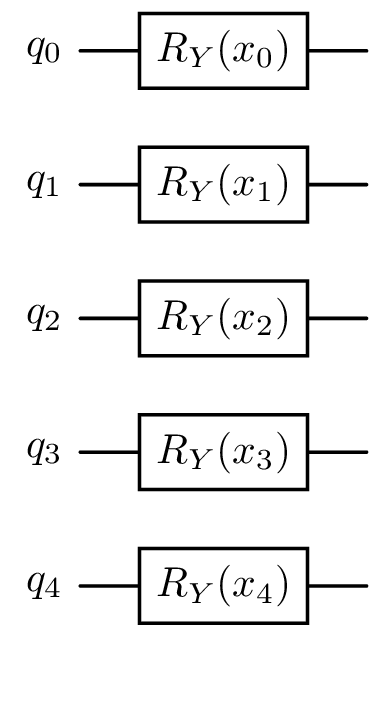
\includegraphics[width=\textwidth]{../images/encoders/quantikz/A1.png}
	%               \caption{}
	%               \label{fig:A1}
	%       \end{subfigure}%
%       \hfill
%       \begin{subfigure}{0.3\textwidth}
	%               \centering
	%               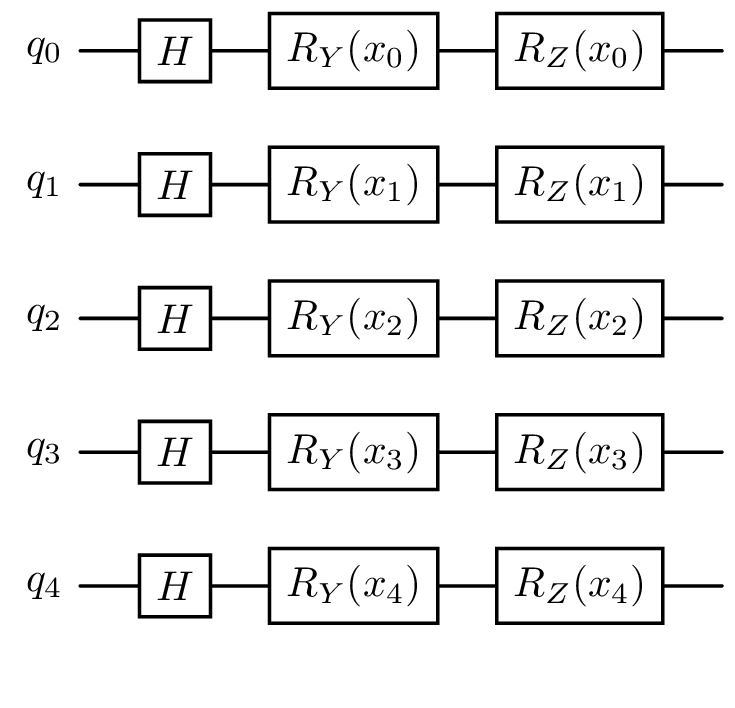
\includegraphics[width=\textwidth]{../images/encoders/quantikz/A2.png}
	%               \caption{}
	%               \label{fig:A2}
	%       \end{subfigure}%
%       \hfill
%       \begin{subfigure}{0.3\textwidth}
	%               \centering
	%               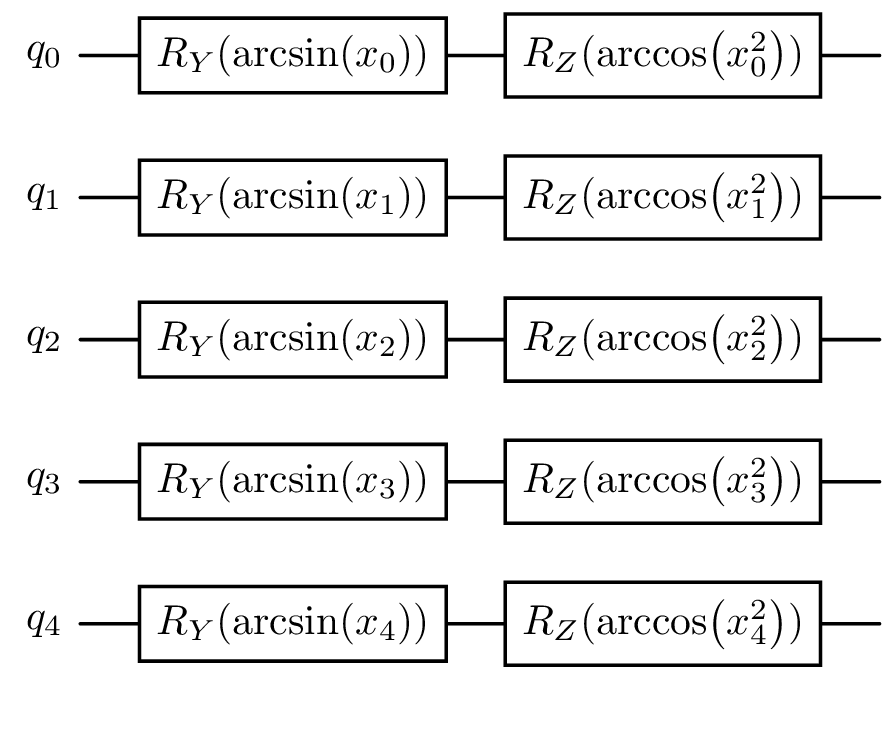
\includegraphics[width=1\textwidth]{../images/encoders/quantikz/M.png}
	%               \caption{}
	%               \label{fig:M}
	%       \end{subfigure}%
%       \hfill
%       \begin{subfigure}{1\textwidth}
	%               \centering
	%                   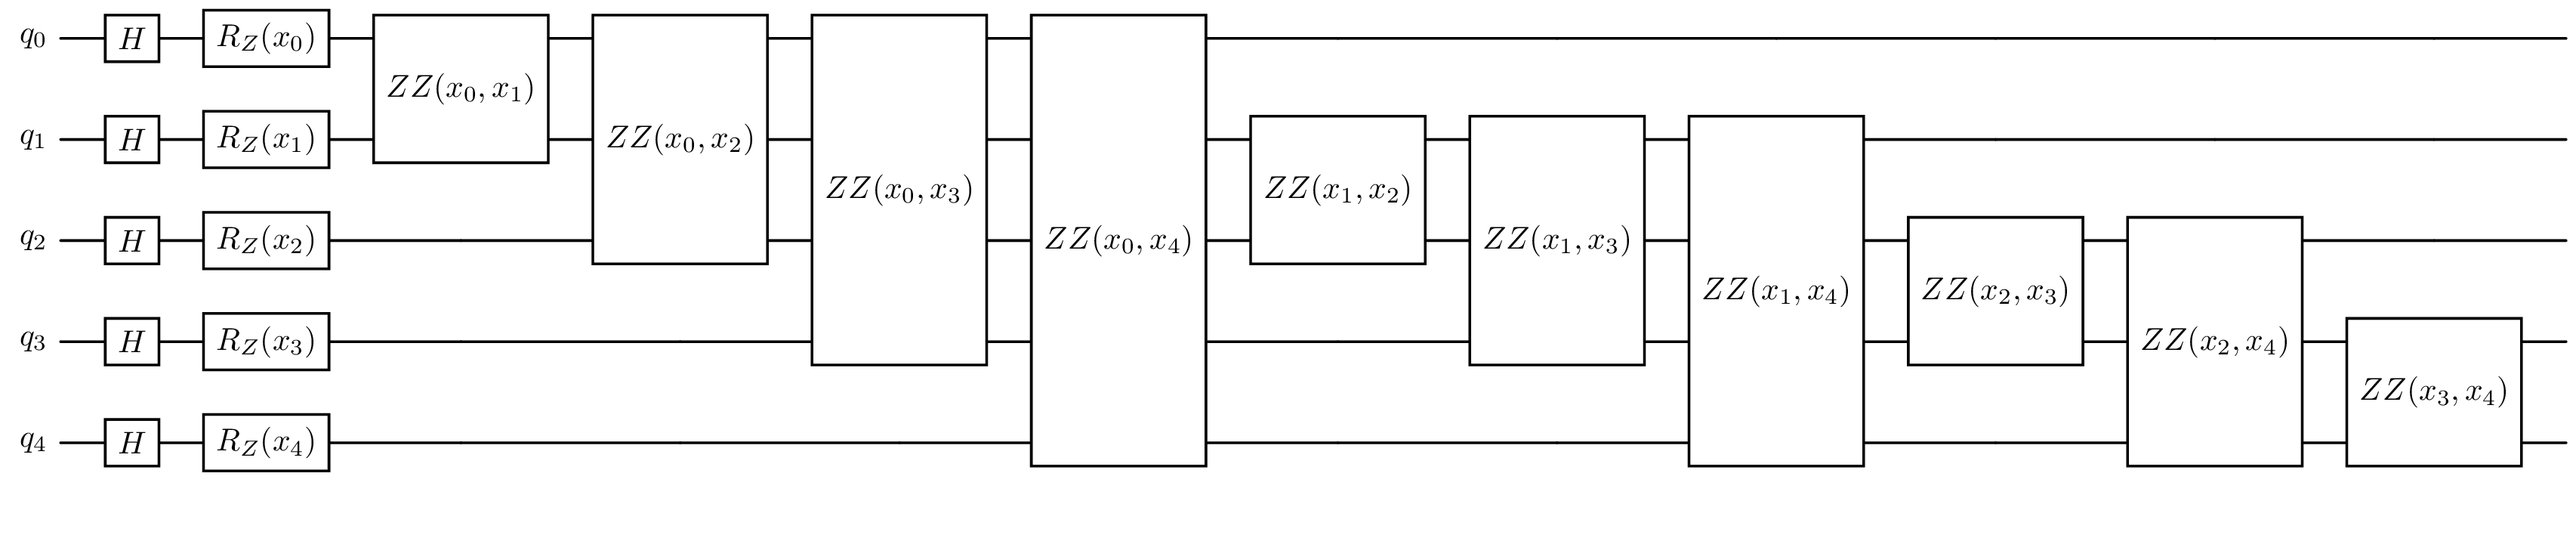
\includegraphics[width=\textwidth]{../images/encoders/quantikz/IQP.png}
	%               \caption{}
	%               \label{fig:IQP}
	%       \end{subfigure}%
%       \caption{(a) Single angle (A1) encoding, (b) double angle (A2) encoding, (c) Mitarai (M) encoding, and (d) Instantaneous Quantum Polynomial (IQP) encoding}
%       \label{fig:encoders}
%\end{figure}



  
\begin{figure}[H]
	\centering
	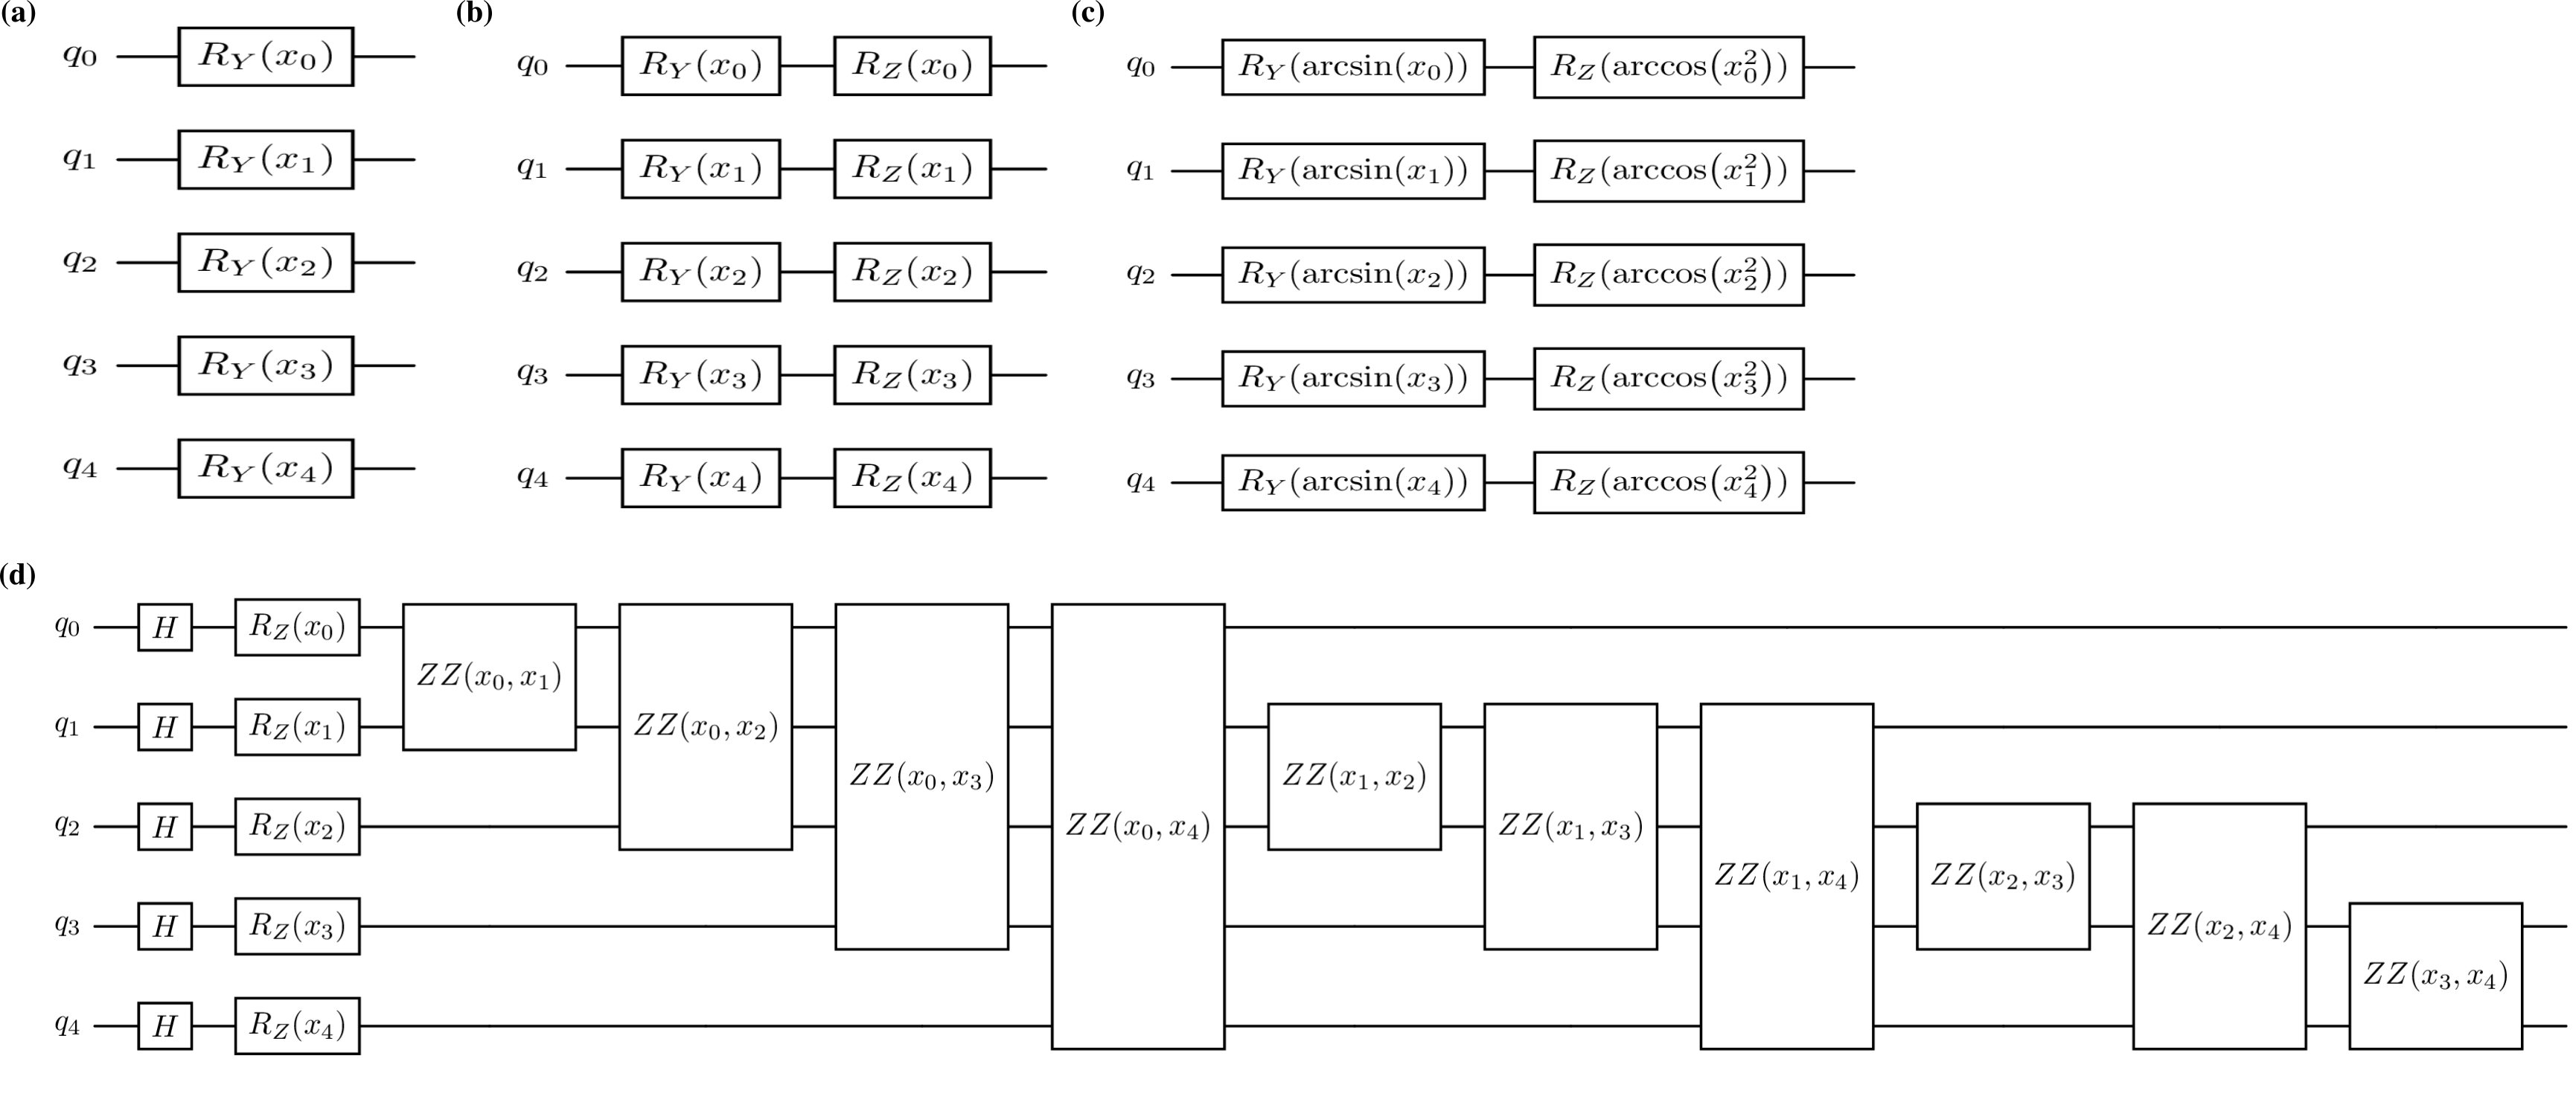
\includegraphics[width=\textwidth]{../images/encoders/quantikz/combined.png}
	\caption{(a) Single angle (A1) encoding, (b) double angle (A2) encoding, (c) Mitarai (M) encoding, and (d) Instantaneous Quantum Polynomial (IQP) encoding}
	\label{fig:encoders}
\end{figure}





  
When $l=2$, like in Ref. \citep{suzuki_predicting_2020} we choose entanglement gates, $E_{\text{ent}}^{1}$ and $E_{\text{ent}}^{2}$ to be equivalent, and the encoding layer takes the following form, $U_{\Phi(x)} =  E_{\text{ent}} U_{\phi_{2}(\mathbf{x})} E_{\text{ent}} U_{\phi_{1}(\mathbf{x})}$ .
We also exclude IQP encoding when $l=2$ due to the increased circuit depth, when compared to A1, A2, and M encoding.
Therefore, there are five unique combinations of $U_{\phi_{1}(\mathbf{x})}$ and $U_{\phi_{2}(\mathbf{x})}$ (M-M, A1-A1, A2-A2, M-A1, and M-A2) and two different entanglement layer options (CNOT and CZ) for a total of 10 encoding circuits. 
These circuits are denoted as $U_{\phi_{1}(\mathbf{x})}-U_{\phi_{2}(\mathbf{x})}-E_{\text{ent}}$, for example, two example encoding circuits are M--M--CNOT and M--A1--CNOT.
Table \ref{tab:encoders} shows all fourteen encoding circuits examined in this study.

\begin{table}[htbp]
	\centering
	\begin{tabular}{|c|c|c|c|}
		\hline
		\textbf{Name} & $U_{\phi_{1}(\mathbf{x})}$ & $U_{\phi_{2}(\mathbf{x})}$ & $E_{\text{ent}}$  \\
		\hline
		\hline
		A1 & $U_{\text{A1}}$ & --- & --- \\
		\hline
		A2 & $U_{\text{A2}}$ & --- & --- \\
		\hline		
		M & $U_{\text{M}}$ & --- & --- \\
		\hline
		IQP & $U_{\text{IQP}}$ & --- & --- \\
		\hline
		A1--A1--CNOT & $U_{\text{A1}}$ & $U_{\text{A1}}$ & $E_{\text{CNOT}}$ \\
		\hline
		 A2--A2--CNOT & $U_{\text{A2}}$ & $U_{\text{A2}}$ & $E_{\text{CNOT}}$ \\
		\hline
		M--M--CNOT & $U_{\text{M}}$ & $U_{\text{M}}$ & $E_{\text{CNOT}}$ \\
		\hline
		M--A1--CNOT & $U_{\text{M}}$ & $U_{\text{A1}}$ & $E_{\text{CNOT}}$ \\
		\hline		
		M--A2--CNOT & $U_{\text{M}}$ & $U_{\text{A2}}$ & $E_{\text{CNOT}}$ \\
		\hline				
		A1--A1--CZ & $U_{\text{A1}}$ & $U_{\text{A1}}$ & $E_{\text{CZ}}$ \\
		\hline
		A2--A2--CZ& $U_{\text{A2}}$ & $U_{\text{A2}}$ & $E_{\text{CZ}}$ \\
		\hline
		M--M--CZ & $U_{\text{M}}$ & $U_{\text{M}}$ & $E_{\text{CZ}}$ \\
		\hline
		M--A1--CZ & $U_{\text{M}}$ & $U_{\text{A1}}$ & $E_{\text{CZ}}$ \\
		\hline		
		M--A2--CZ & $U_{\text{M}}$ & $U_{\text{A2}}$ & $E_{\text{CZ}}$ \\
		\hline						
	\end{tabular}
	\caption{Add something smart}
	\label{tab:encoders}
\end{table}



Following the encoding layers,variational (or ansatz) layers are used to introduce trainable parameters into the quantum circuit.
We use a mixed notation from Refs. \citep{suzuki_predicting_2020} and \citep{sim_expressibility_2019}, since Ref. \citep{sim_expressibility_2019} contains all of the variational layers used within this work.
We relegate the discussion of the expressibility and entanglement examined in that work to Section \ref{section:results_and_discussion}.
A general variational layer can be denoted as,
\begin{equation}
	U(\bm{\theta}) = \prod_{v} U_{v}(\bm{\theta}_{v}), % E_{\text{ent}}^{v}
	\label{eq:general_variational}
\end{equation}
where $\bm{\theta}$ denotes the variational parameters and $v$ denotes the number of times that the layer is repeated within the circuit. 
As $v$ increases and the number of trainable parameters ($\bm{\theta}$) increase, the theoretical assumption is that the model expressibility should also increase.
In our study, we choose $v \in \{1, 3, 5\}$ and refer to this as the number of ansatz layers (ALs).
We examine 12 different variational circuits, as shown in Fig. \ref{fig:ansatz}, which are denoted using the following labels: Modified-Pauli-CRZ (Fig. \ref{fig:ansatz}\textbf{(a)}) , Modified-Pauli-CRX (Fig. \ref{fig:ansatz}\textbf{(b)}), Efficient-CRZ (Fig. \ref{fig:ansatz}\textbf{(c)}), Efficient-CRX (Fig. \ref{fig:ansatz}\textbf{(d)}),, HWE-CNOT (Fig. \ref{fig:ansatz}\textbf{(e)}), HWE-CZ (Fig. \ref{fig:ansatz}\textbf{(f)}), ESU2 (Fig. \ref{fig:ansatz}\textbf{(g)}), Full-Pauli-CRZ (Fig. \ref{fig:ansatz}\textbf{(h)}), Full-Pauli-CRX (Fig. \ref{fig:ansatz}\textbf{(i)}), Hadamard (Fig. \ref{fig:ansatz}\textbf{(j)}), Full-CRZ (Fig. \ref{fig:ansatz}\textbf{(k)}), and Full-CRX (Fig. \ref{fig:ansatz}\textbf{(l)}),

\begin{figure}[H]
	\centering
	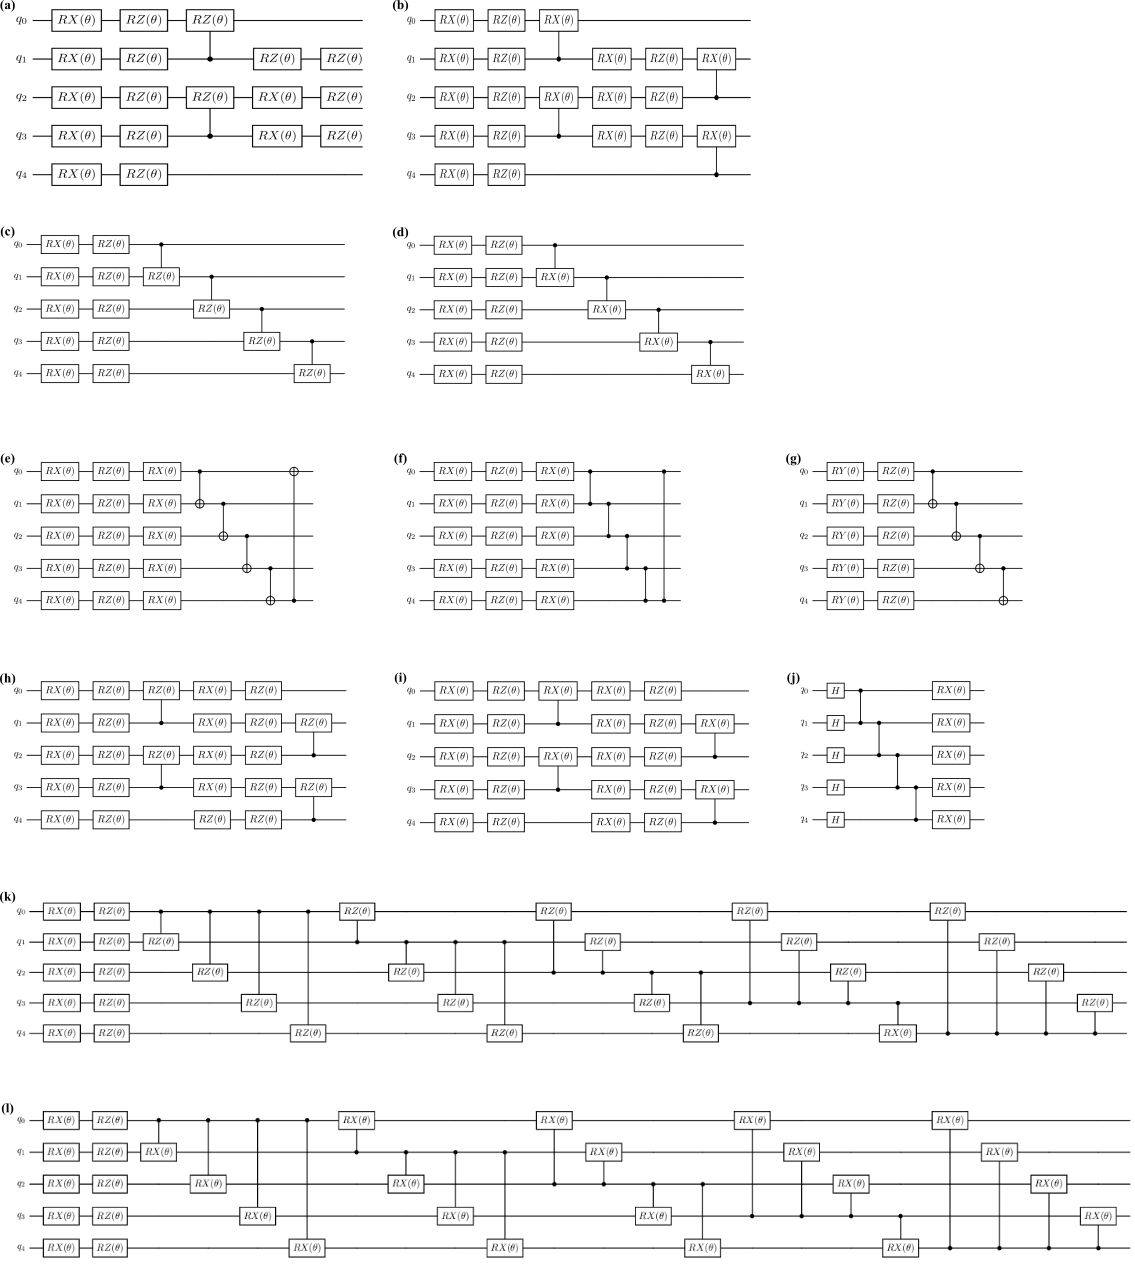
\includegraphics[width=\textwidth]{../images/ansatz/quantikz/combined.png}
	\caption{(a) Modified-Pauli-CRZ, (b) Modified-Pauli-CRX, (c) Efficient-CRZ, (d) Efficient-CRX, (e) HWE-CNOT, (f) HWE-CZ,  (g) ESU2, (h) Full-Pauli-CRZ, (i) Full-Pauli-CRX, (j) Hadamard, (k) Full-CRZ, and (l)Full-CRX}
	\label{fig:ansatz}
\end{figure}

Now that we have define the encoding (Eq. \ref{eq:general_encoding}) and variational (Eq. \ref{eq:general_variational}) circuits, we can then combine them to denote a general, complete circuit as,
\begin{equation}
	\ket{\Psi} = U(\bm{\theta}) U_{\Phi(\mathbf{x})}\ket{0}^{\otimes n} = \prod_{k}
	\left( \prod_{v} U_{v}(\bm{\theta}_{v}) \prod_{l} E_{\text{ent}}^{l} U_{\phi_{l}(\mathbf{x})} \right)  \ket{0}^{\otimes n},
\end{equation}
where we choose $k \in \{1, 3, 5\}$, which denotes the re-upload depth (RUD) of the circuit.
When a sufficient number of data re-uploading occur, it has been shown by P\'{e}rez-Salinas \textit{et al.} that data re-uploading is equivalent to the Universal Approximation Theorem for artificial neural networks.\cite{perez-salinas_data_2020}


Lastly, to recover the predicted target values, $\hat{y}_{i}$, from our quantum circuits, measurement of the quantum state, $\ket{\Psi}$, must be performed.
To perform this operation, we apply the Pauli Z operator on the first qubit denoted as,
\begin{equation}
	\hat{y}_{i} = \bra{\Psi}Z_{0}\ket{\Psi}_{i}.
	\label{eq:y_pred}
\end{equation}
The set of predicted target values, $\bm{\hat{y}} = (\hat{y}_{1}, \ldots, \hat{y}_{N}) \in \mathbb{R}^{N}$, where $N$ is the number of samples, is then passed to the loss function, $\mathcal{L}(\bm{y}, \bm{\hat y})$, where $y_{i}$ belongs to the set of true target values $\bm{y} = (y_{1}, \ldots, y_{N}) \in \mathbb{R}^{N}$.
In practice, $\mathcal{L}$ can be any loss function but we choose to use the mean square error loss function denoted as,
\begin{equation}
	\mathcal{L}(\bm{y}, \bm{\hat y}) = \frac{1}{N} \sum_{i=1}^{N} (y_{i} - \hat{y}_{i})^{2}.
	\label{eq:isthisloss}
\end{equation}


\subsection{Implementation}
\begin{figure}[H]
	\centering
	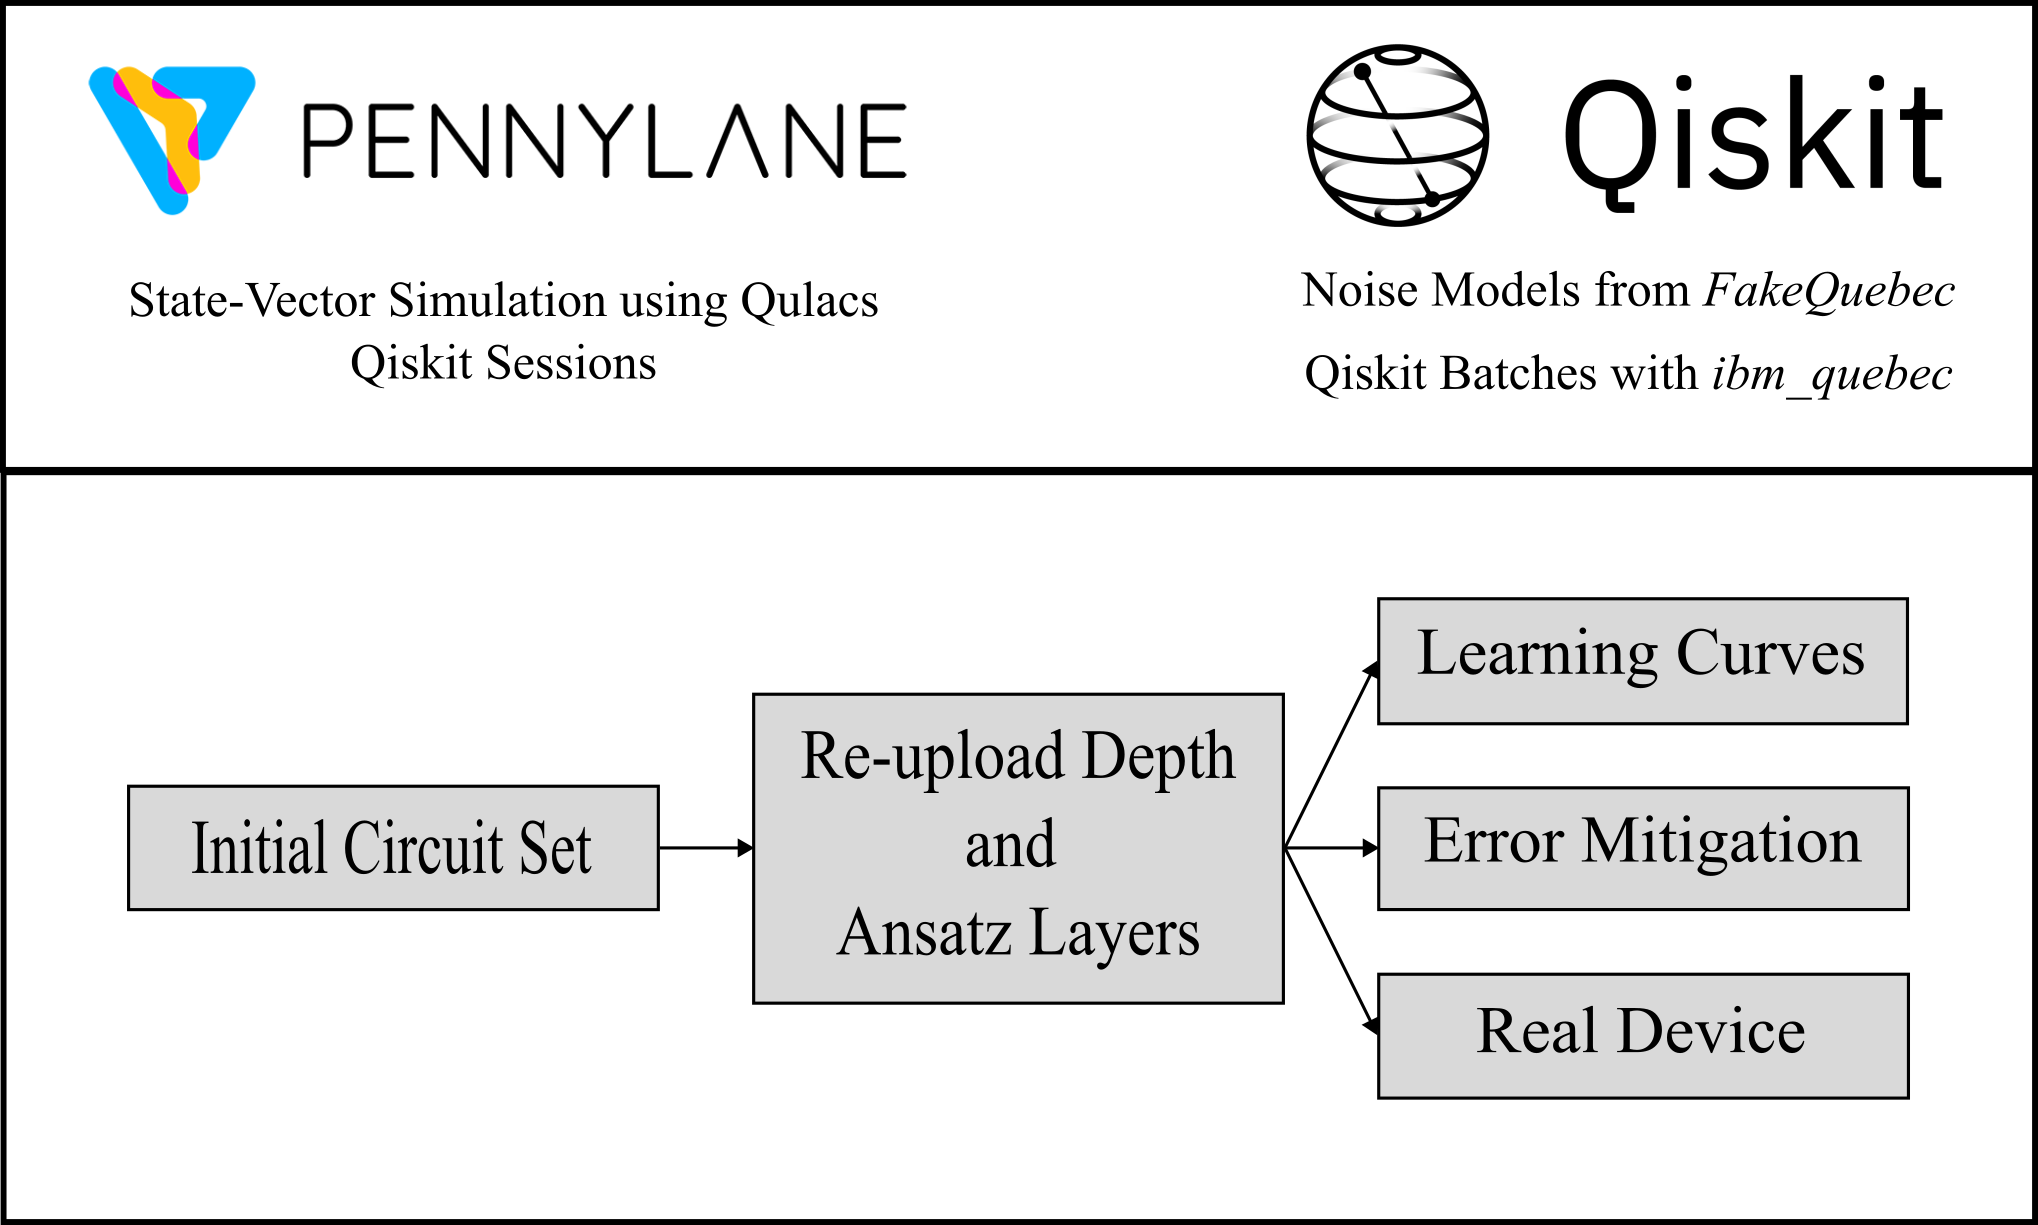
\includegraphics[width=\linewidth]{../images/manuscript_figures/overview.png}
	\caption{Make this figure highlight the modularity of \textit{qregress}}
	\label{fig:overview_project}
\end{figure}

We introduce \textit{qregress}, a modular Python package for regression-based PQCs.

We perform all simulation calculations using PennyLane\cite{bergholm_pennylane_2022}, either using Qulacs\cite{suzuki_qulacs_2021} for state vector calcualtions, while noisy calculations were performed using \textit{qiskit-aer} with the \textit{FakeQuebec} backend as implemented in the PennyLane-Qiskit plugin.\cite{javadi-abhari_quantum_2024}
We perform calculations in the \textit{ibm\_quebec} device using circuits implemented using Qiskit\cite{javadi-abhari_quantum_2024}, due to issues we initially faced with running experiments on the real device using the PennyLane-Qiskit plugin.
For the experiments using PennyLane,  we utilize the Simultaneous Perturbation Stochastic Approximation method (SPSA) as implemented in PennyLane, while for the experiments run on \textit{ibm\_quebec} utilizes the Constrained Optimization By Linear Approximation (COBYLA) optimizer as implemented ing SciPy\cite{virtanen_scipy_2020}.
Each optimizer was chosen based on the performance for the given task.
All features ($\mathbf{x}$) and target values ($\mathbf{y}$) were scaled using the MinMaxScaler in Scikit-learn\cite{pedregosa_scikit-learn_2011}, such that all featues and target values are $\mathbb{R}\in [ -1,1 ]$.
For the simulations using \textit{FakeQuebec} and experiments on \textit{ibm\_quebec} we utilize Twirled Readout Error eXtinction (TREX) error mitigation.

Function fitting 5: all ran with 1000 iterations
Function fitting 16: all ran with 1000 iterations
BSE 5: all ran with 1000 iterations
BSE 16: all ran with 1000 iterations
DDCC

\subsection{Datasets}\label{subsection:datasets}
In this study, we explore three datasets: a function fitting dataset (Figs. \ref{fig:linear_train_vs_test},\ref{fig:quadratic_train_vs_test}, and \ref{fig:sine_train_vs_test}), consisting of a noisy functions used for model calibration; a dataset of bond separation energies (BSE) of molecules (Figs. \ref{fig:bondtypes} and \ref{fig:BSEdistr}), where the feature set encodes structural information of each molecule;
and a dataset consisting of electronic structure features to predict wave functions using the data-driven coupled-cluster scheme of Townsend and Vogiatzis (Fig. \ref{fig:waterddccdistribution}).\cite{townsend_data-driven_2019}
We utilize the BSE49 and DDCC databases for two different reasons: the BSE49 database consists of a hard chemical property to predict using few features, while the DDCC dataset can be predicted easily using few features classically but is data intensive in the number of samples per molecule.

\begin{figure}[H]
	\centering
	\begin{subfigure}[b]{0.3\textwidth}
		\centering
		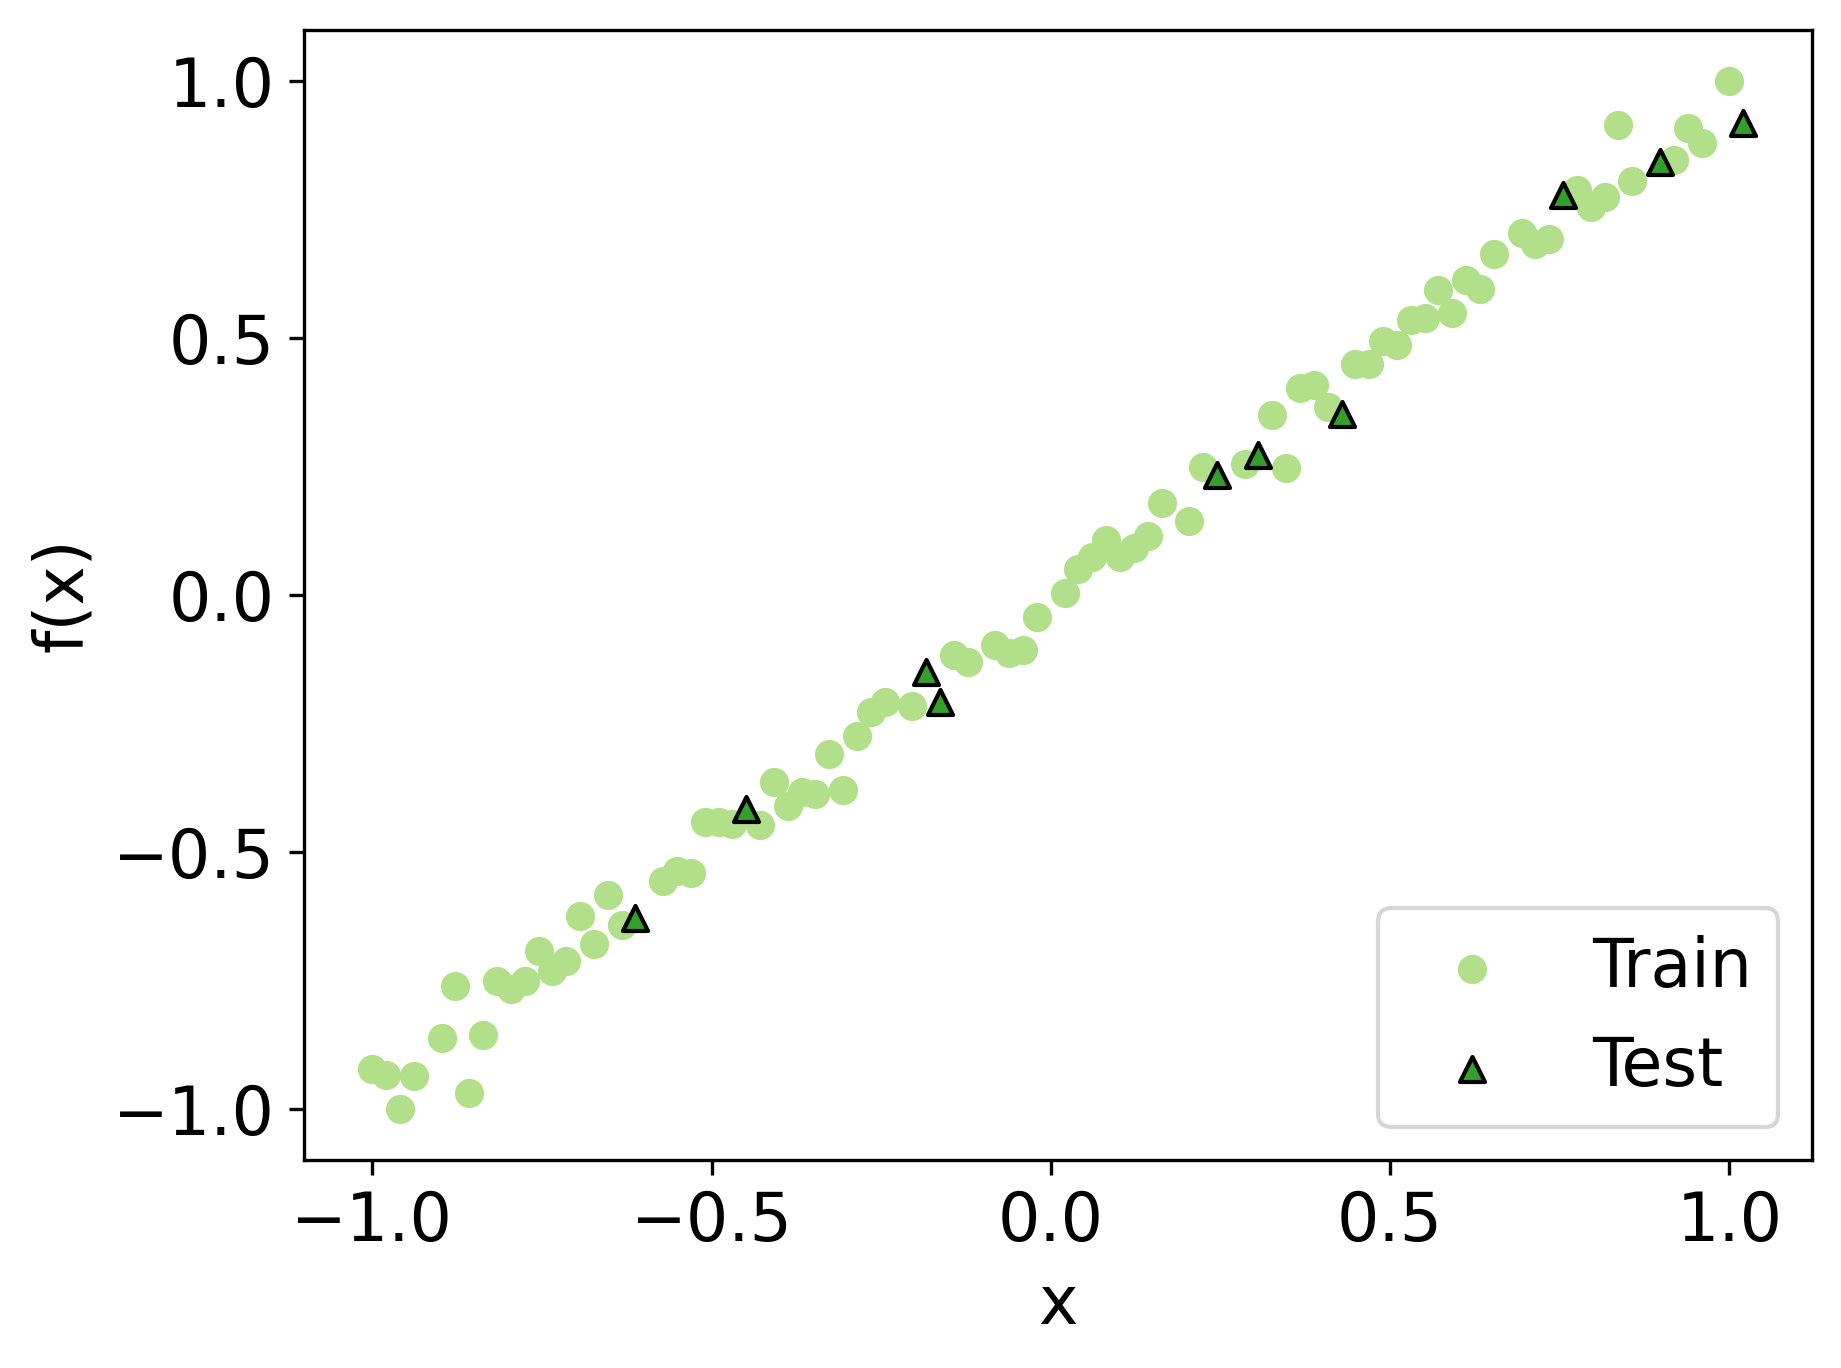
\includegraphics[width=\textwidth]{../images/Function_Fitting/function_dataset/linear_train_vs_test.png}
		\caption{}
		\label{fig:linear_train_vs_test}
	\end{subfigure}
	\hfill
	\begin{subfigure}[b]{0.3\textwidth}
		\centering
		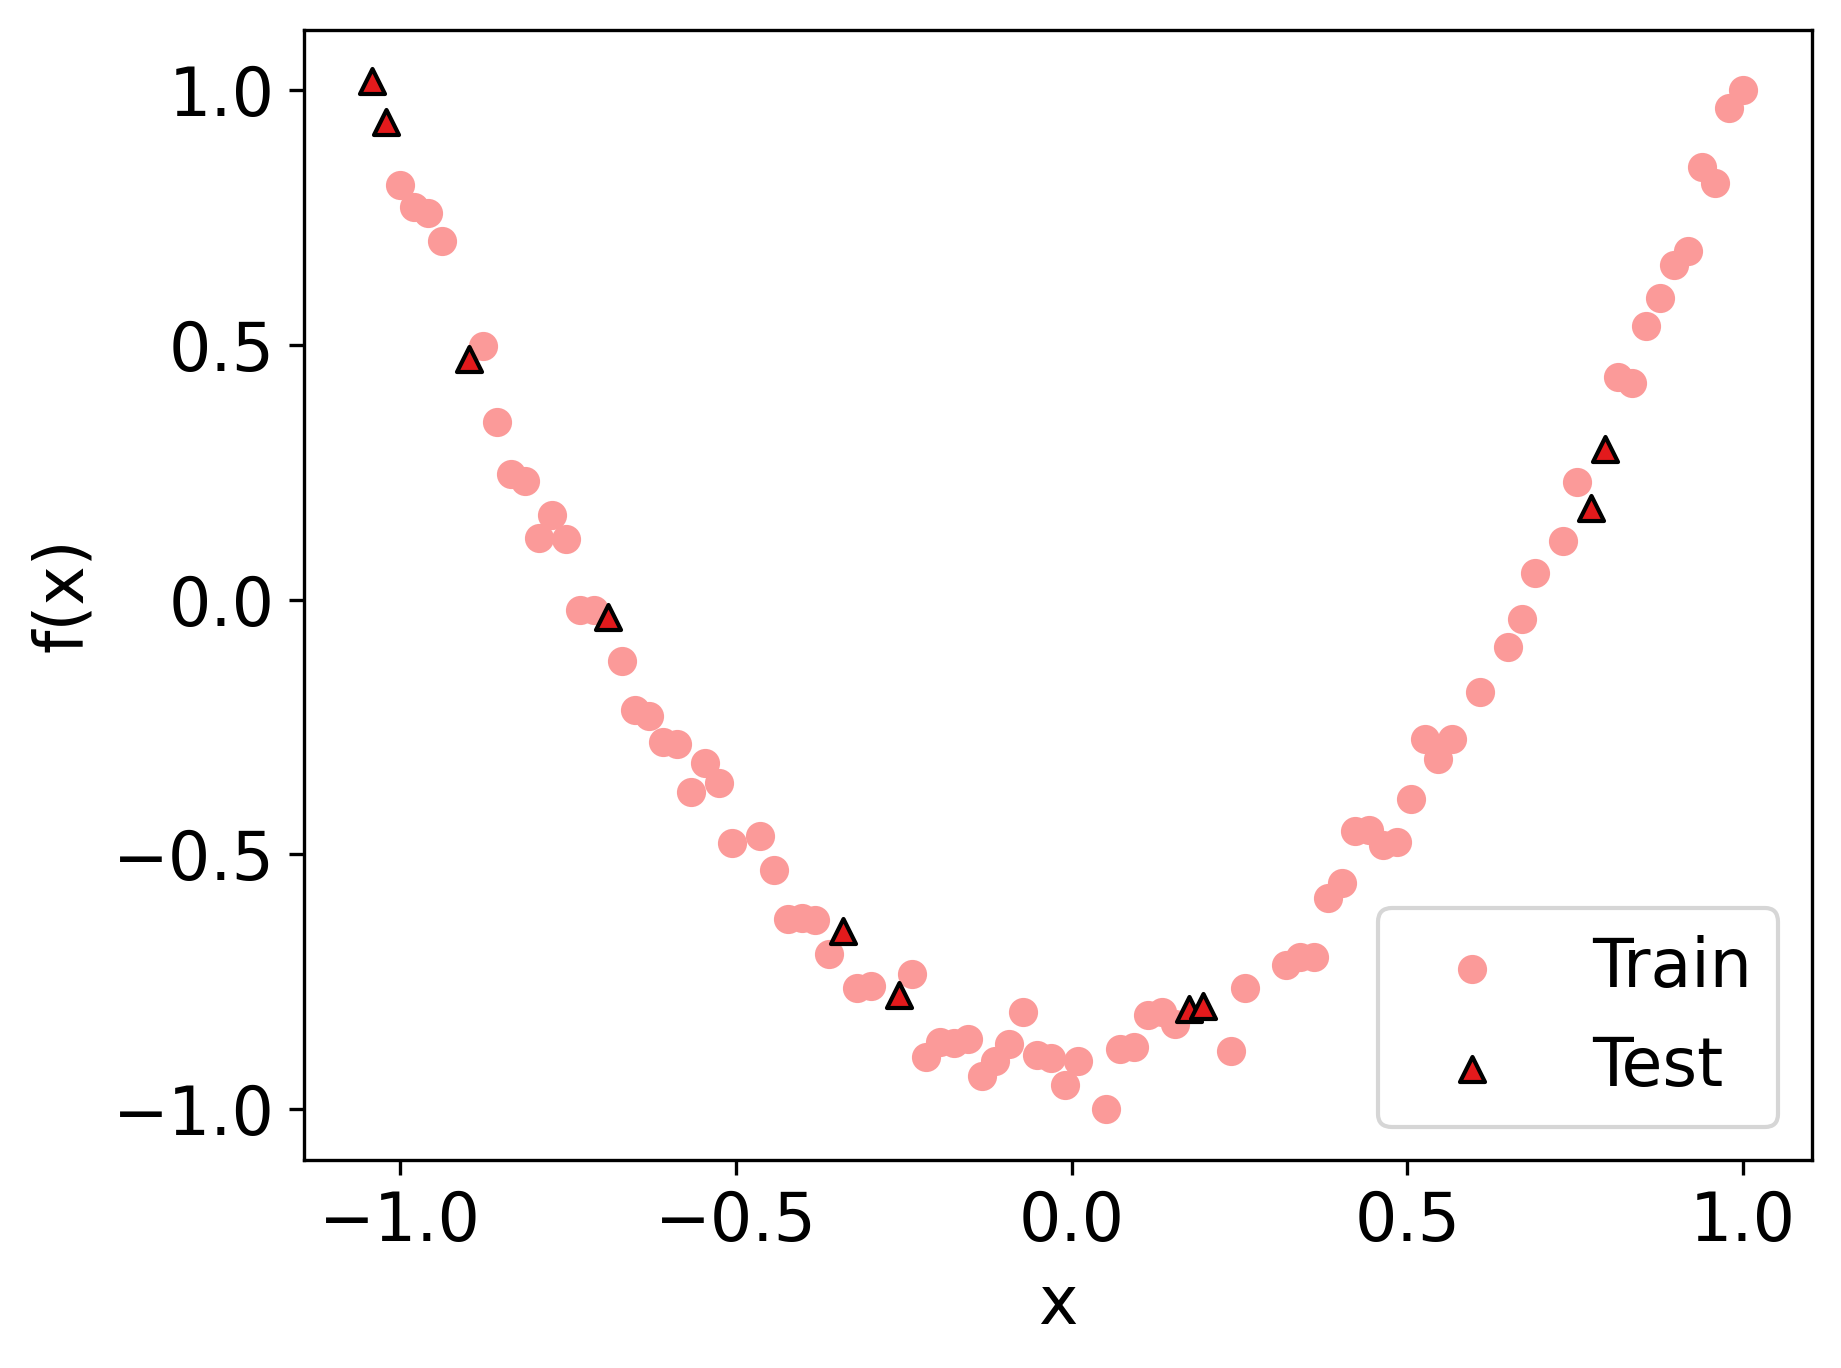
\includegraphics[width=\textwidth]{../images/Function_Fitting/function_dataset/quadratic_train_vs_test.png}
		\caption{}
		\label{fig:quadratic_train_vs_test}
	\end{subfigure}
	\hfill
	\begin{subfigure}[b]{0.3\textwidth}
		\centering
		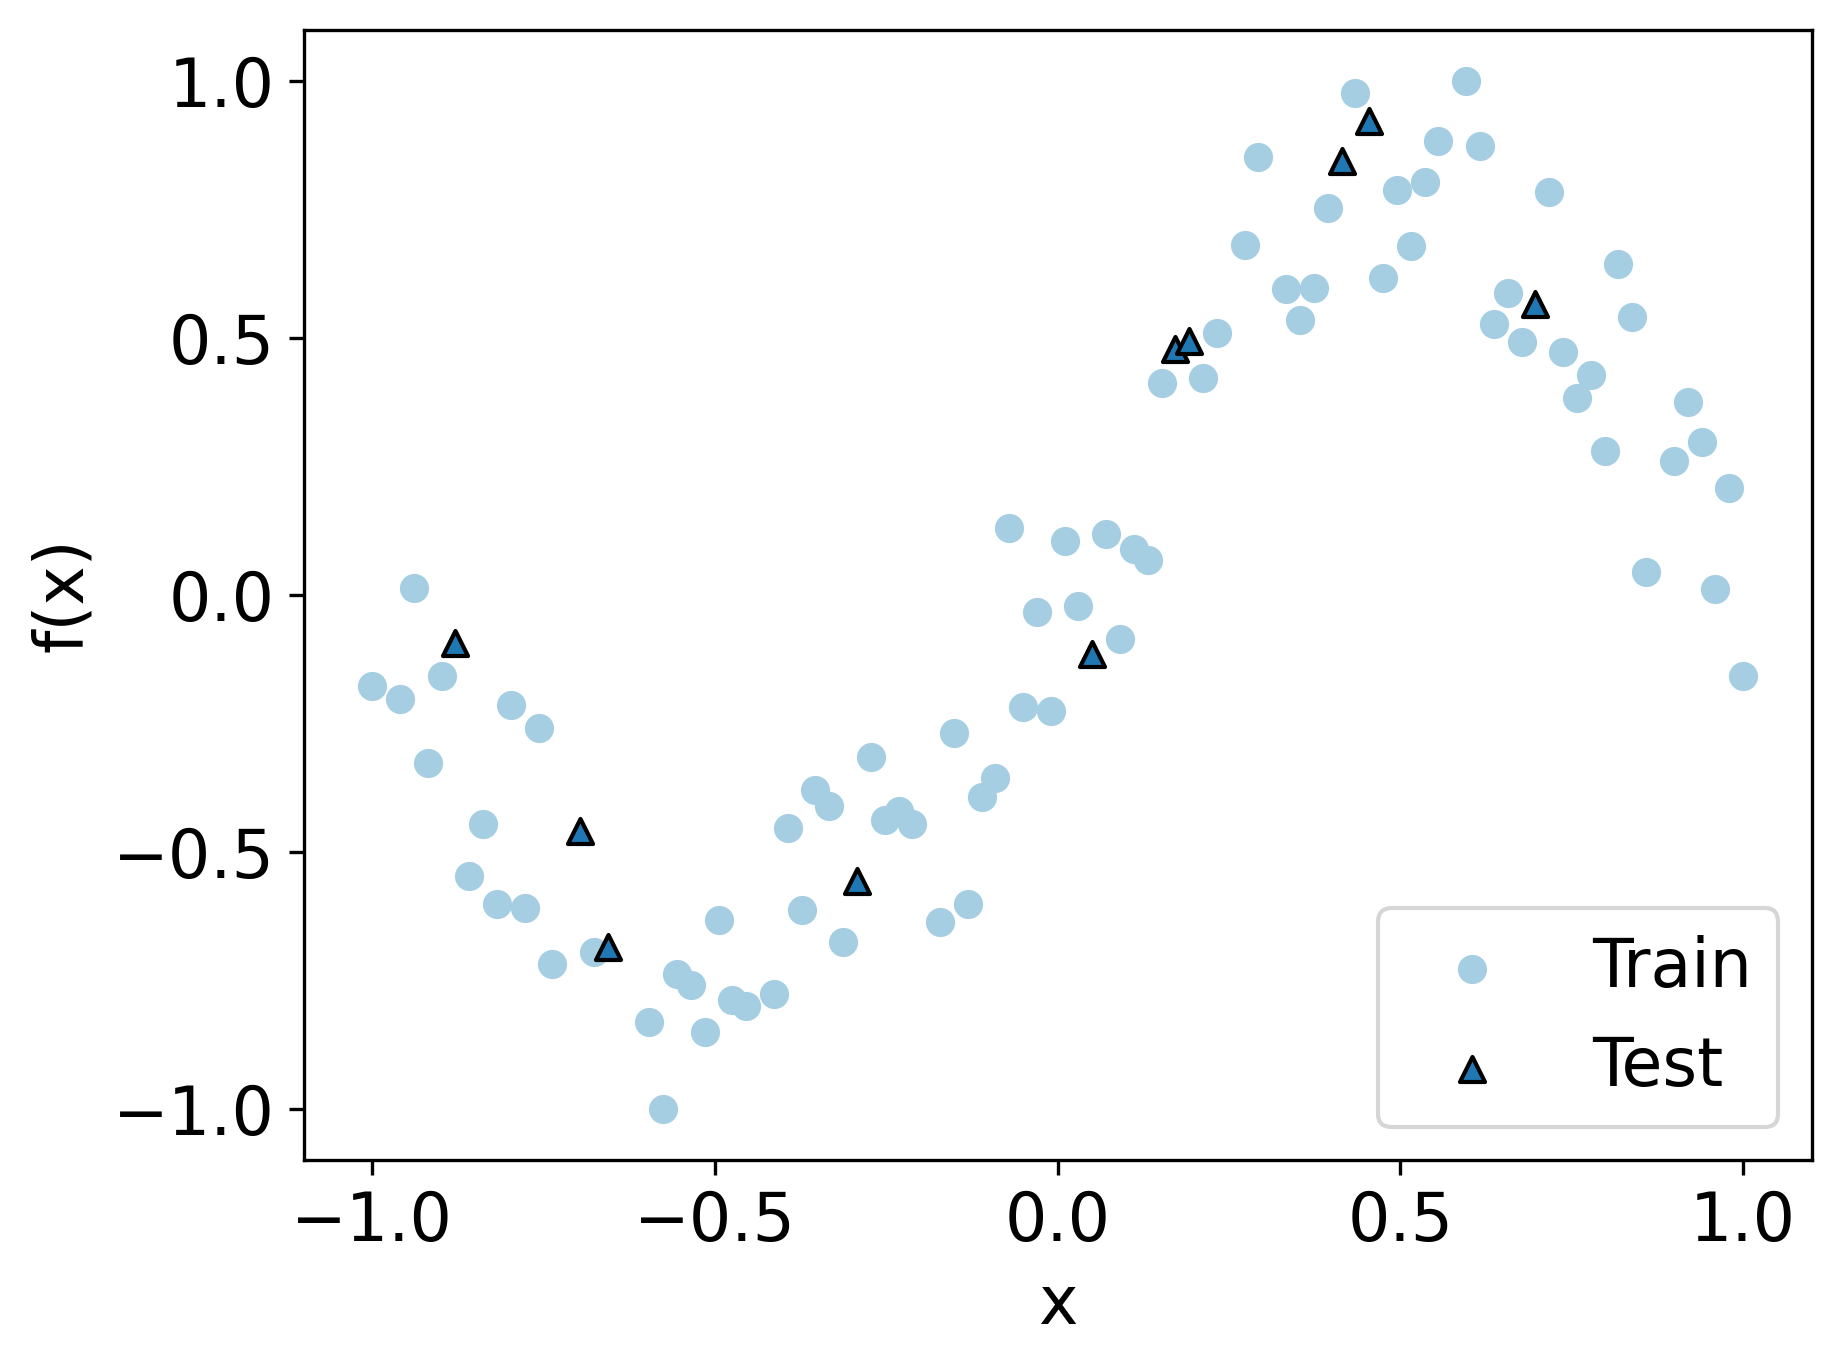
\includegraphics[width=\textwidth]{../images/Function_Fitting/function_dataset/sine_train_vs_test.png}
		\caption{}
		\label{fig:sine_train_vs_test}
	\end{subfigure}	
	\hfill
	\begin{subfigure}[b]{0.65\textwidth}
		\centering
		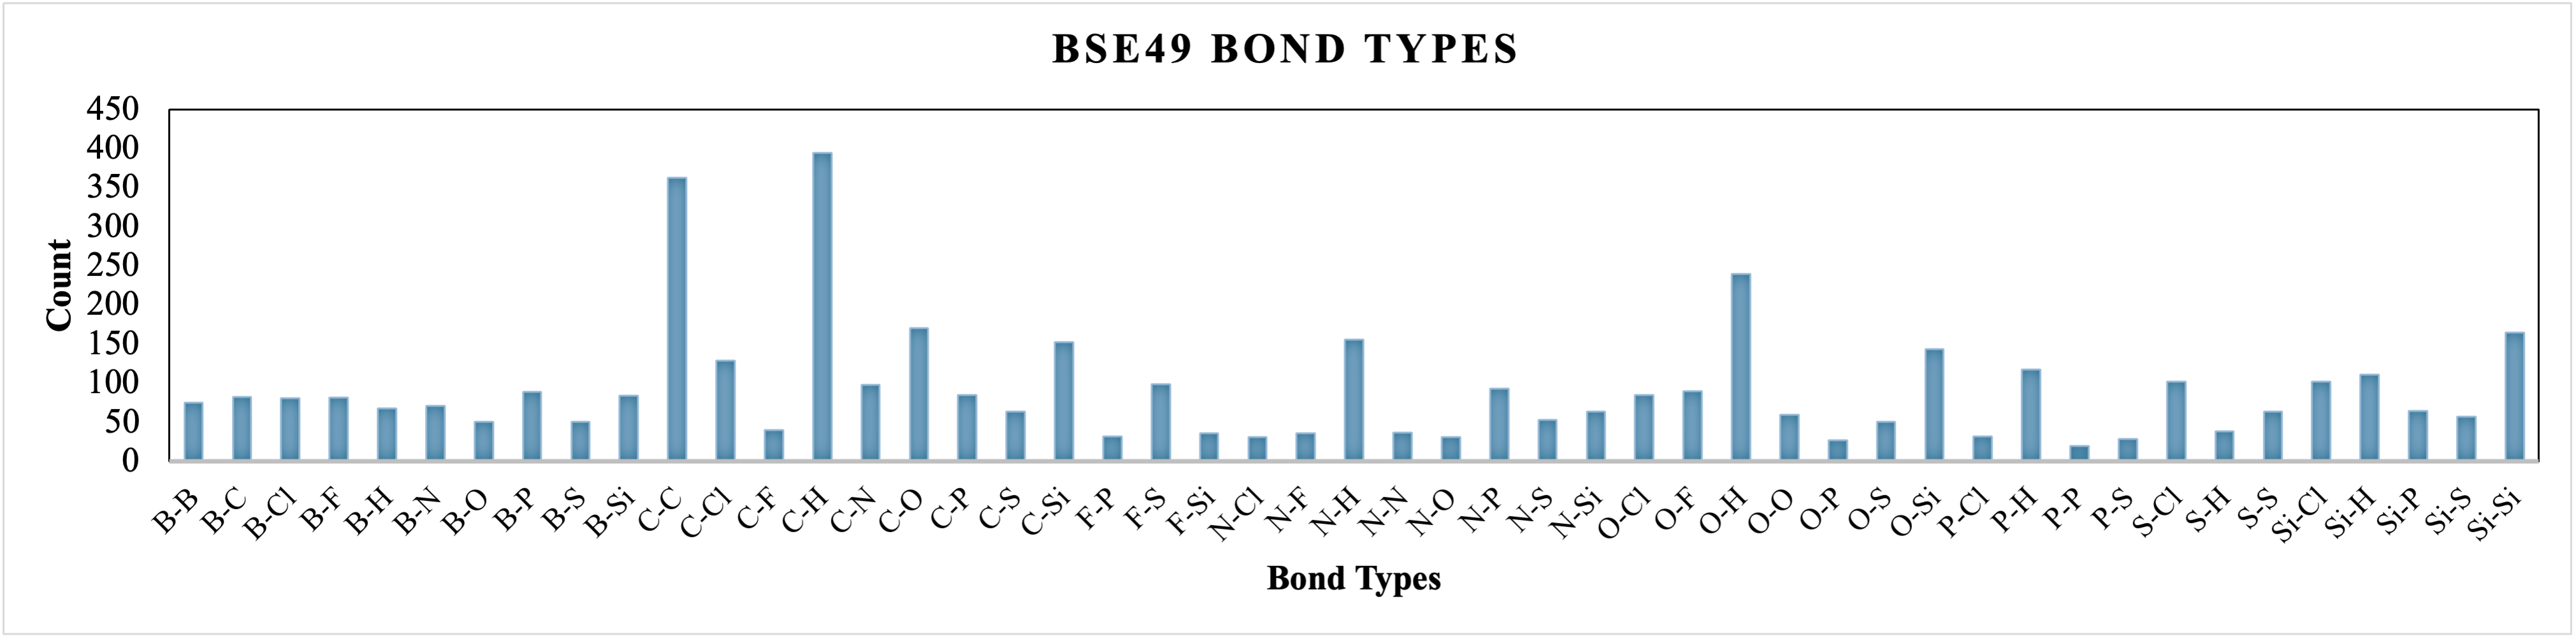
\includegraphics[width=\textwidth]{../images/BSE/bondtypes.png}
		\caption{}
		\label{fig:bondtypes}
	\end{subfigure}
	\hfill
	\begin{subfigure}[b]{0.3\textwidth}
		\centering
		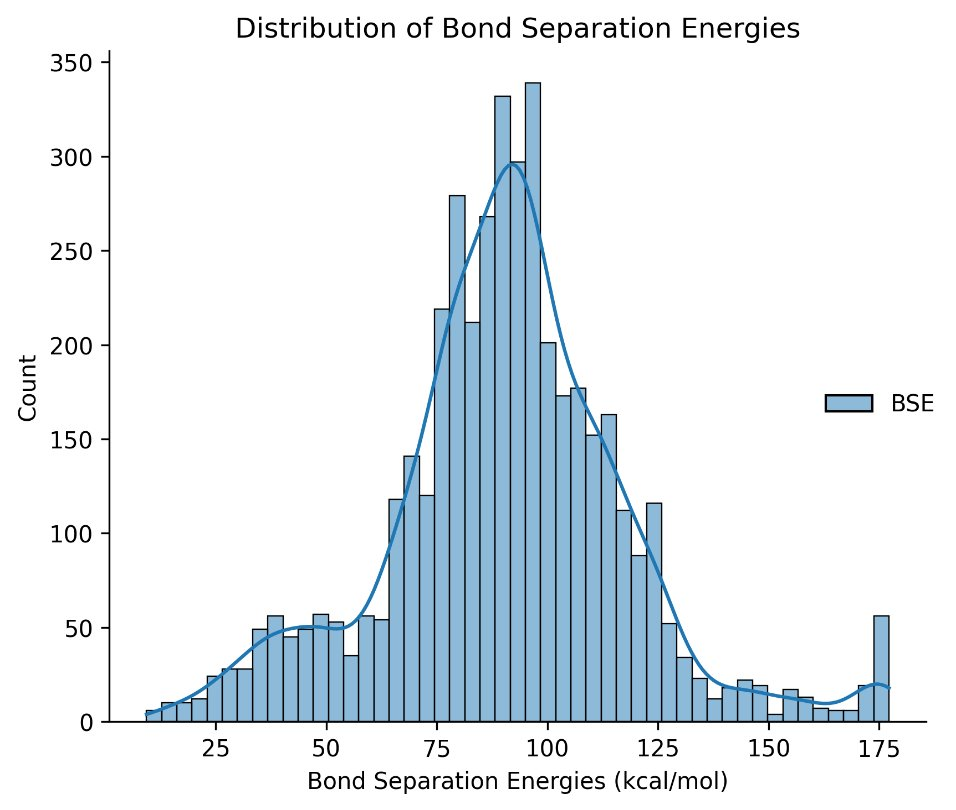
\includegraphics[width=\textwidth]{../images/BSE/BSE.jpg}
		\caption{}
		\label{fig:BSEdistr}
	\end{subfigure}
	\hfill
	\begin{subfigure}[b]{0.3\textwidth}
		\centering
		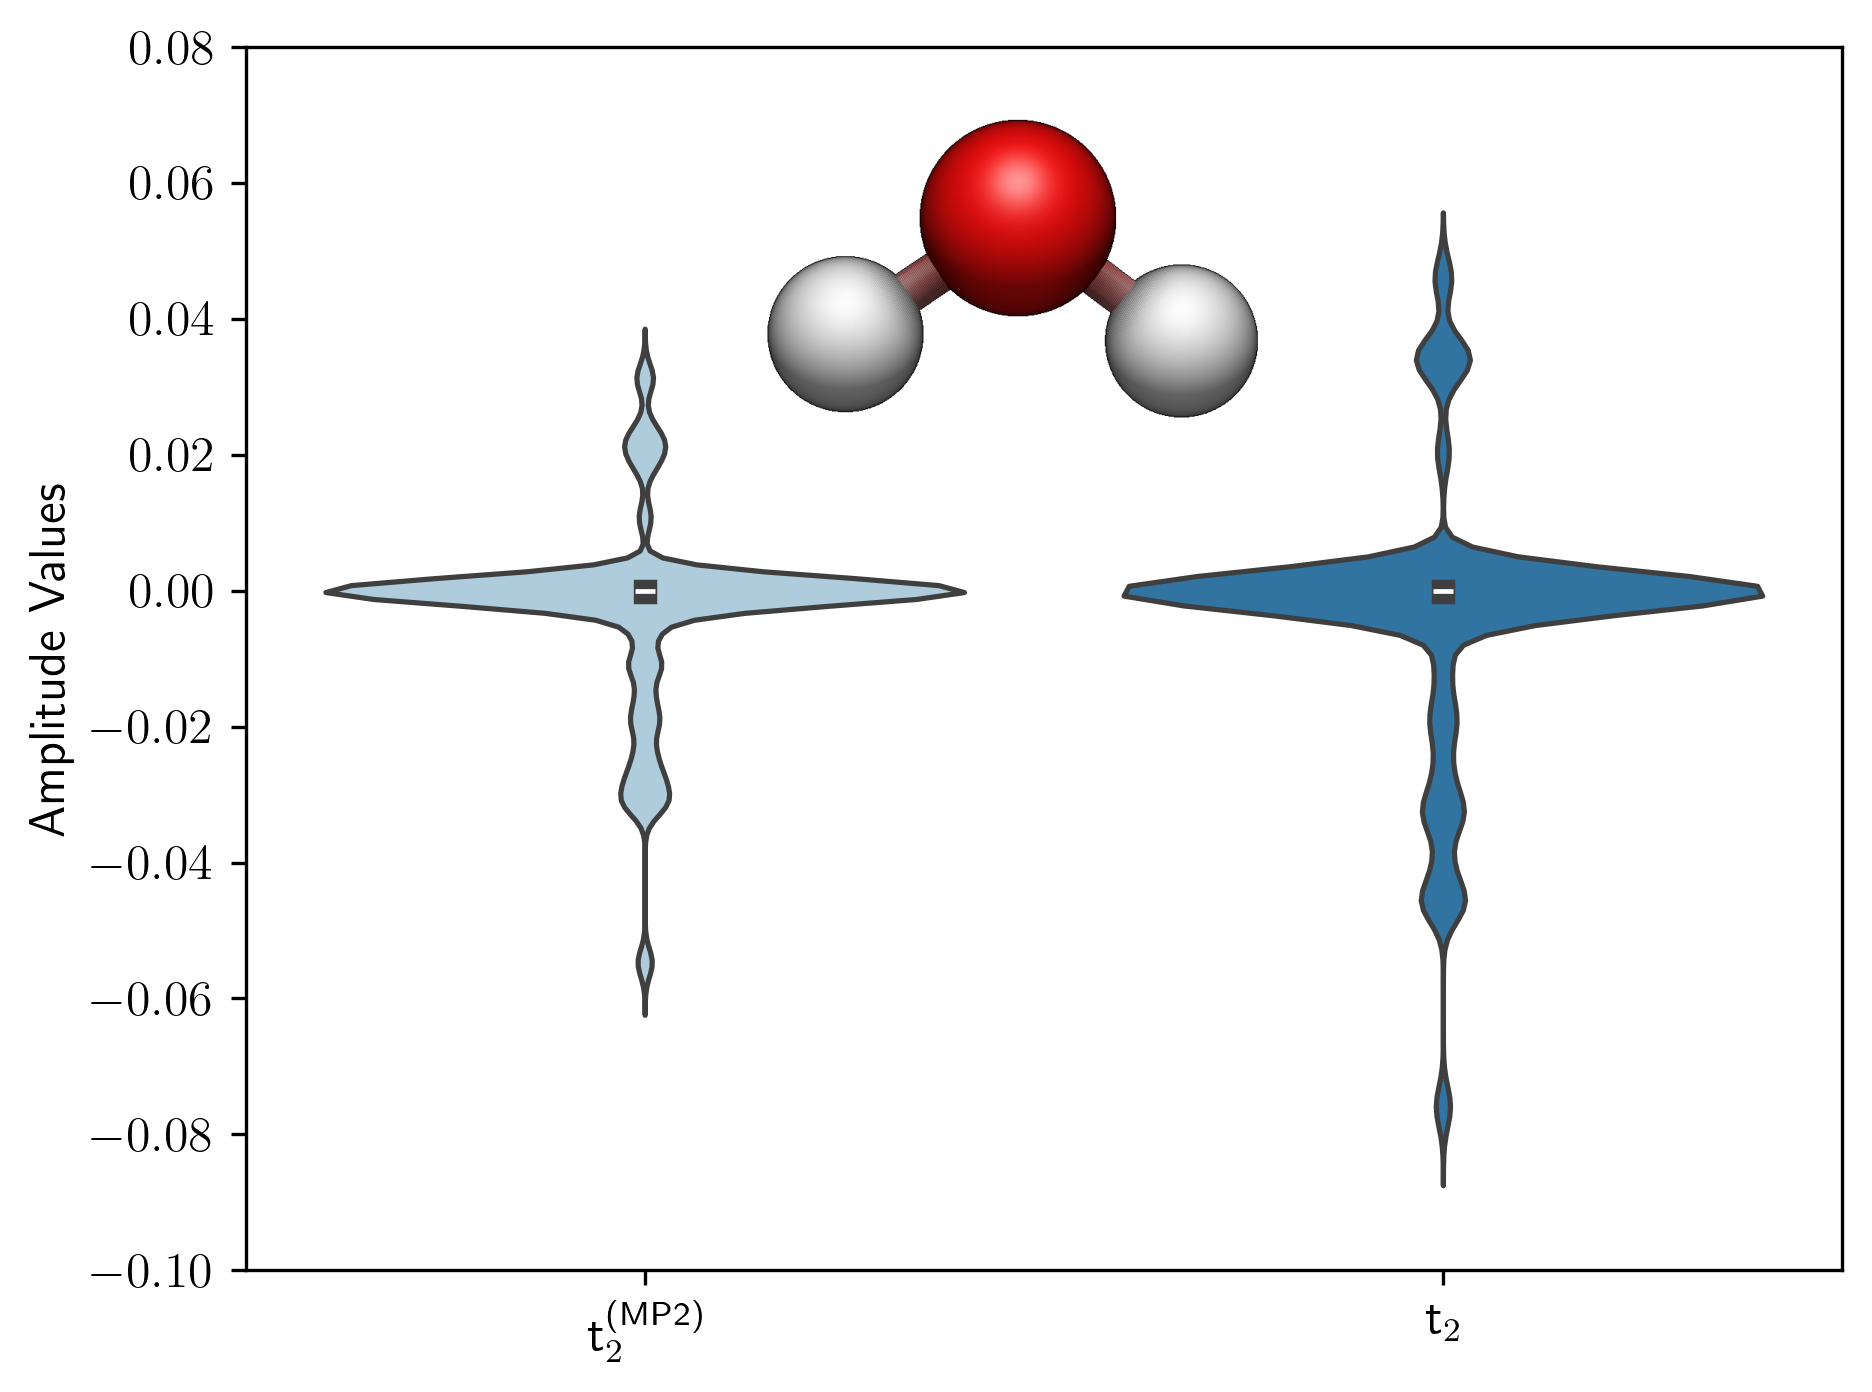
\includegraphics[width=\textwidth]{../images/manuscript_figures/waterddccdistribution.png}
		\caption{}
		\label{fig:waterddccdistribution}
	\end{subfigure}	
	\caption{Examples of the datasets explored in this study. The function fitting dataset used for model calibration include (a) linear (green), (b) quadratic (pink), and (c) sine (blue) functions. For the BSE49 dataset the distributions of the (d) bond types and the (e) bond separation energies in kcal/mol. For the DDCC dataset distributions of the initial MP2 $t_{2}$-amplitudes and the optimized CCSD $t_{2}$-amplitudes are shown in (f).}
	\label{fig:bse_data}
\end{figure}


The function fitting dataset consists of a noisy linear (Fig. \ref{fig:linear_train_vs_test}), quadratic (Fig. \ref{fig:quadratic_train_vs_test}), and sine (\ref{fig:sine_train_vs_test}) function.  
For each function, 90 points are generated, where 80 are used for training set and 10 for the test set.
This dataset is used for calibration of the 168 PQCs, along with providing additional insights into the effects of circuit depth, training set size, and error mitigation on model performance.


%\begin{figure}[H]
%	\centering
%	\begin{subfigure}[b]{0.3\textwidth}
%		\centering
%		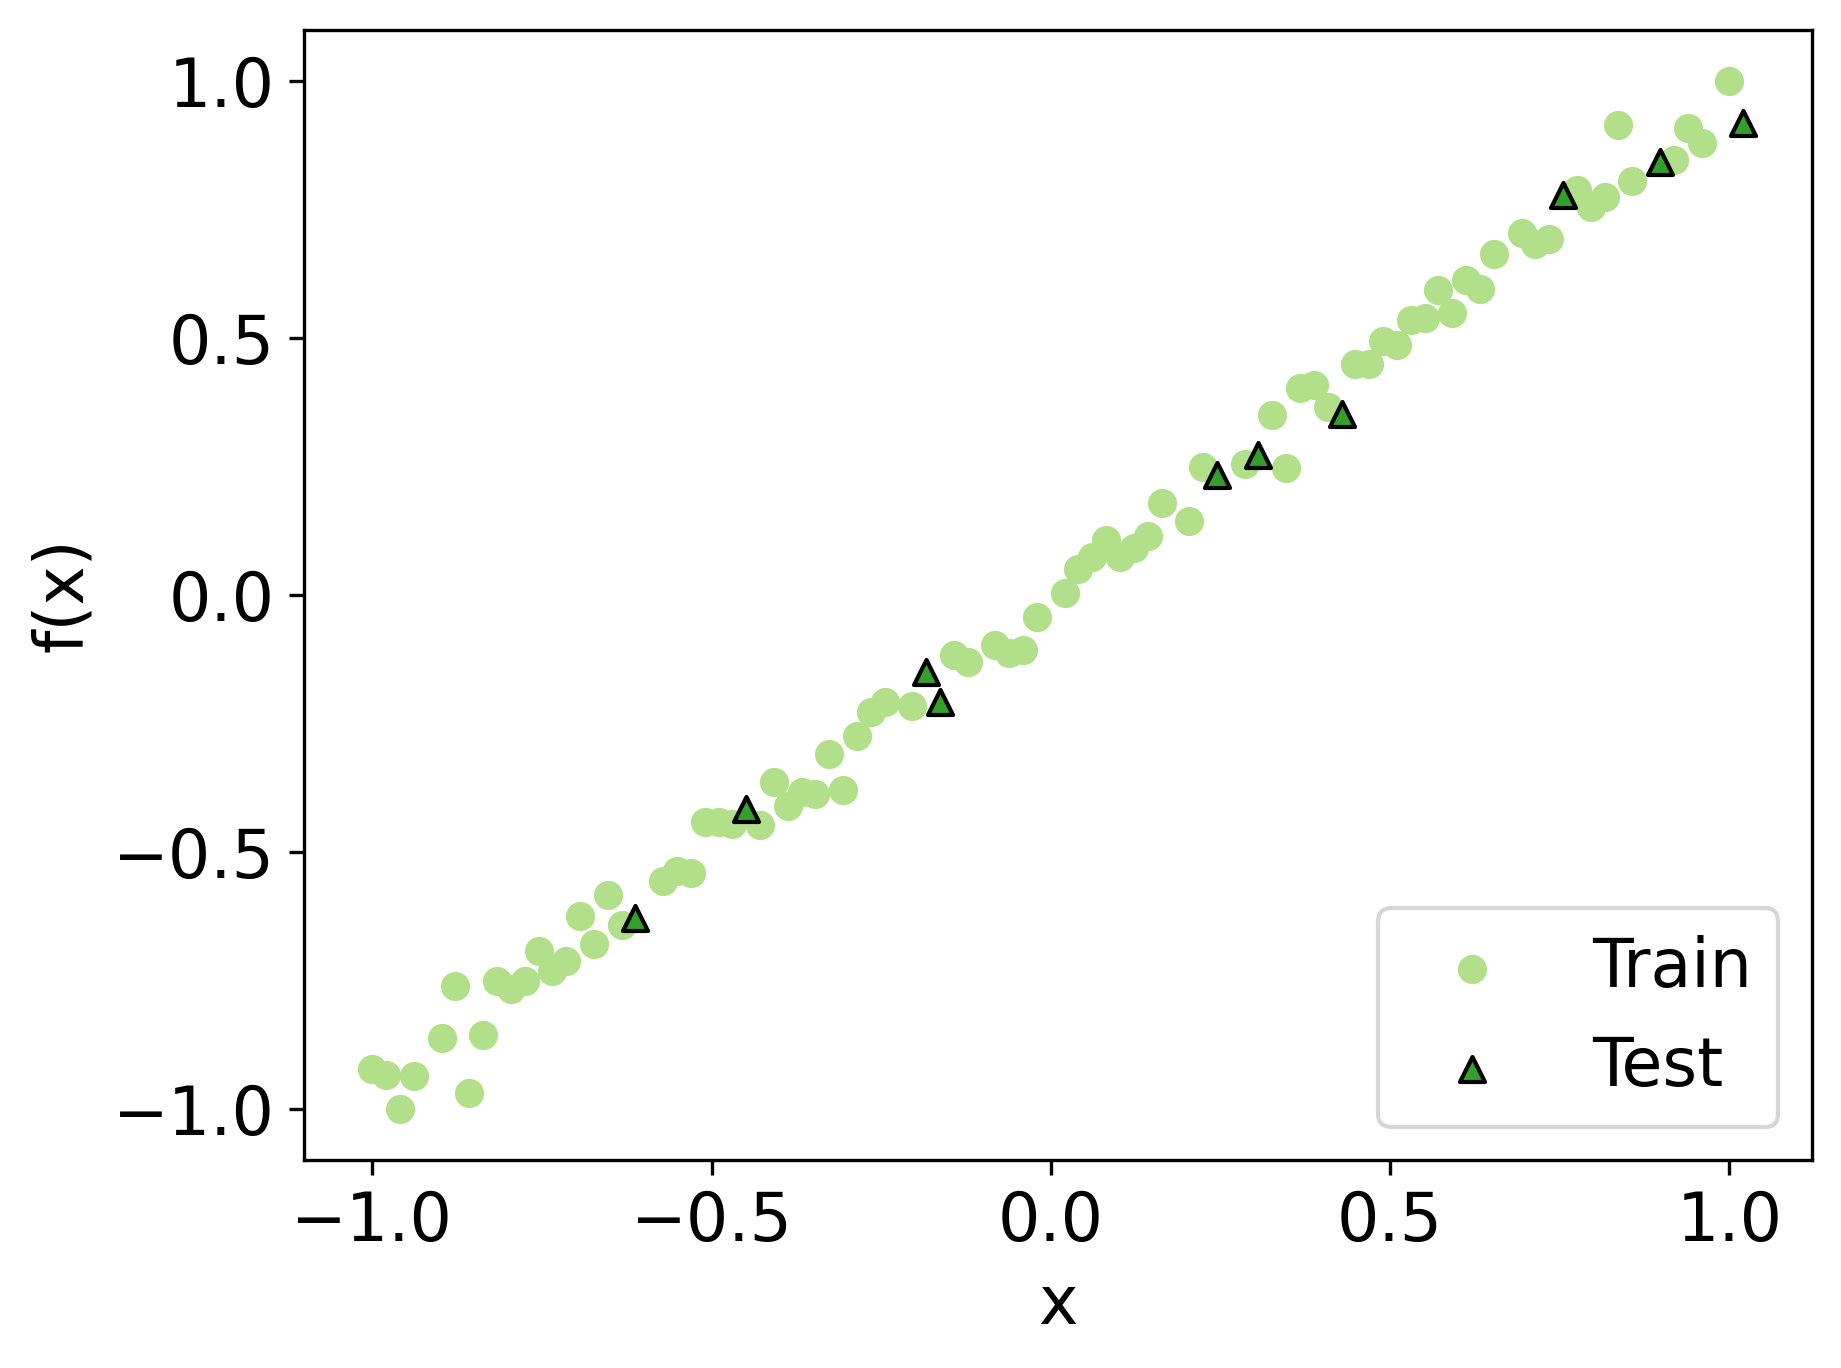
\includegraphics[width=\textwidth]{../images/Function_Fitting/function_dataset/linear_train_vs_test.png}
%		\caption{}
%		\label{fig:linear_train_vs_test}
%	\end{subfigure}
%	\hfill
%	\begin{subfigure}[b]{0.3\textwidth}
%		\centering
%		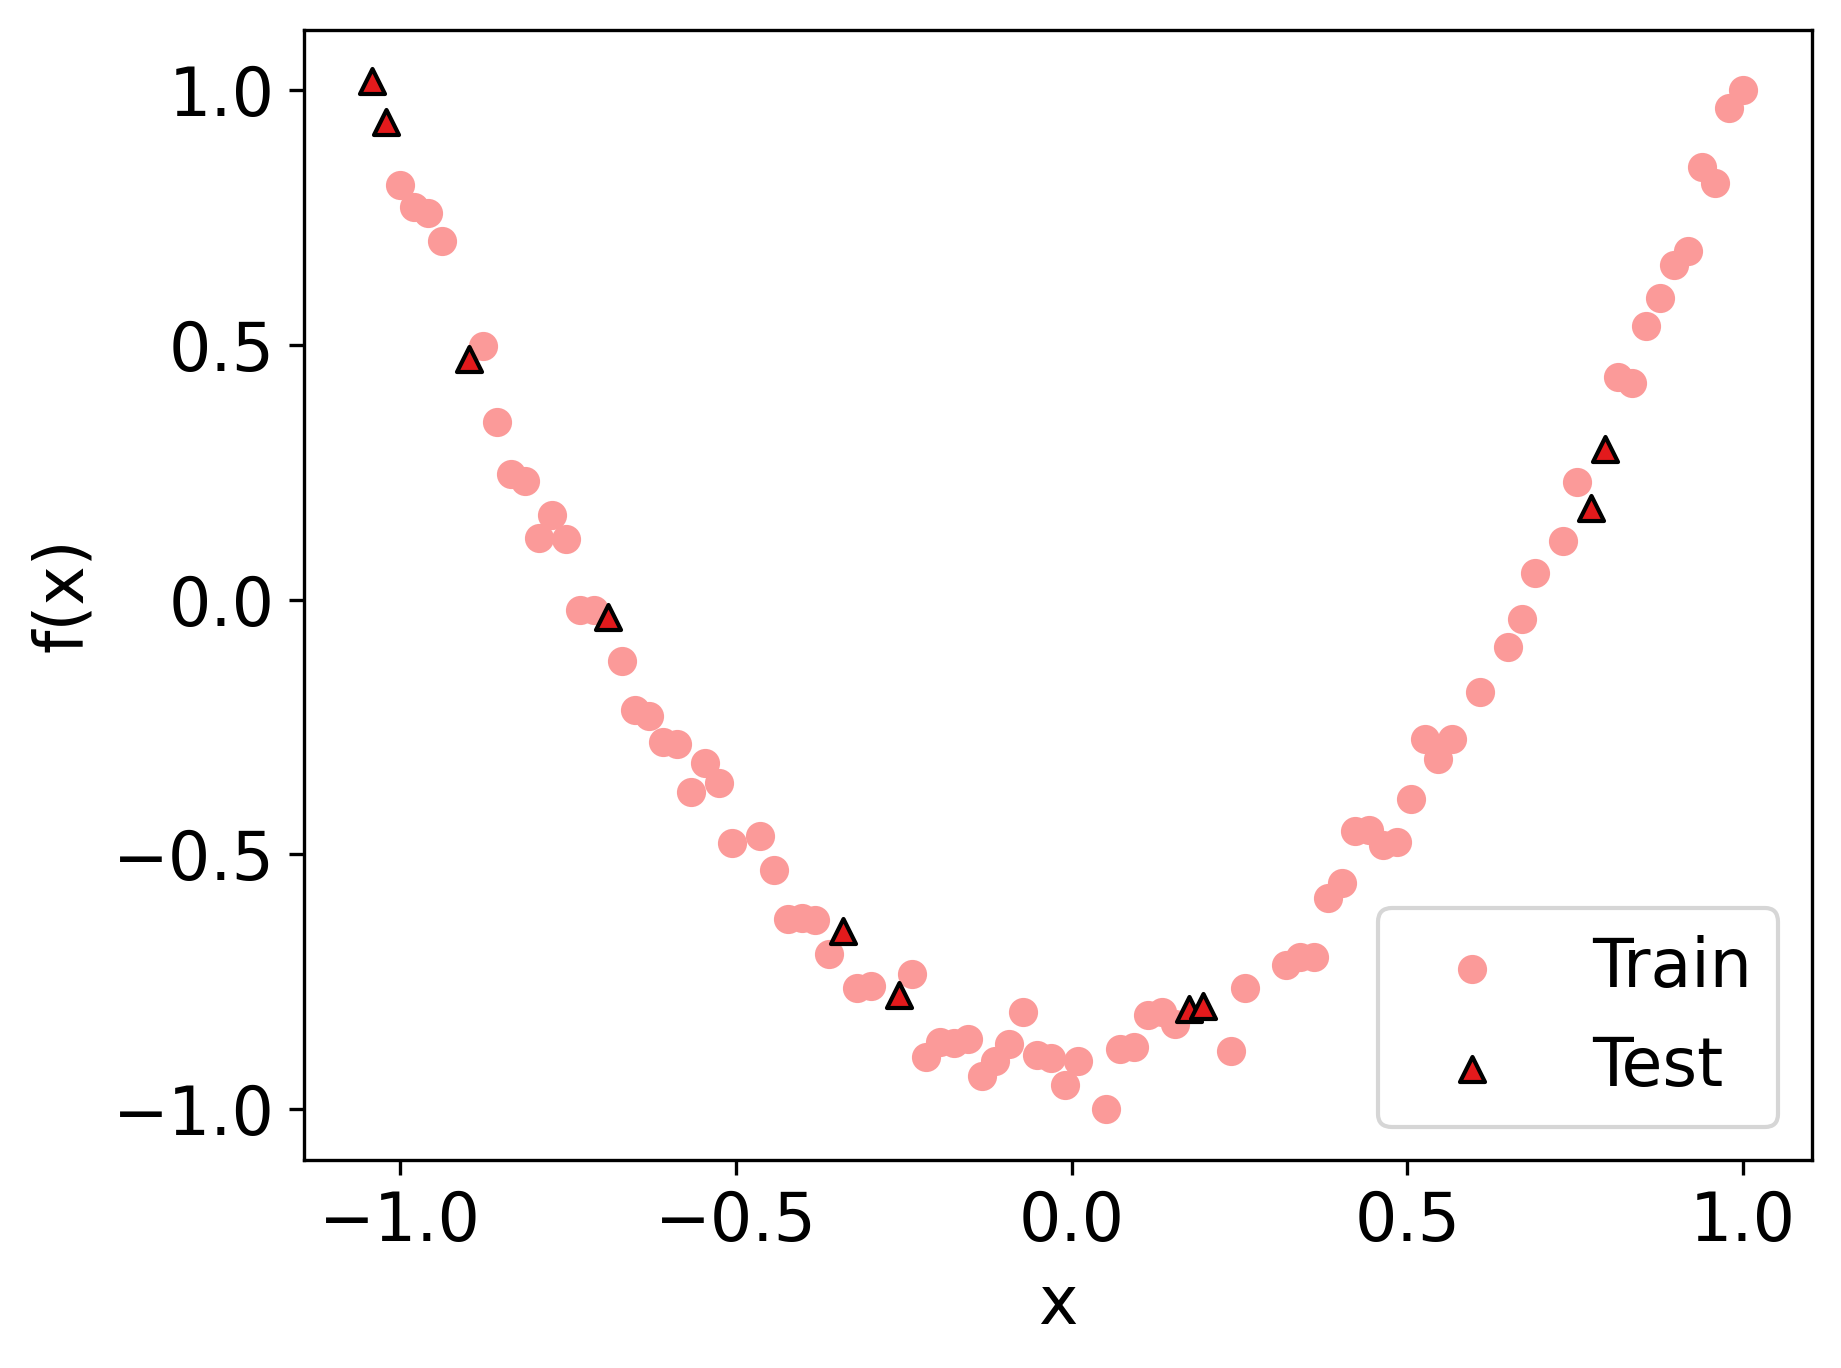
\includegraphics[width=\textwidth]{../images/Function_Fitting/function_dataset/quadratic_train_vs_test.png}
%		\caption{}
%		\label{fig:quadratic_train_vs_test}
%	\end{subfigure}
%	\hfill
%	\begin{subfigure}[b]{0.3\textwidth}
%		\centering
%		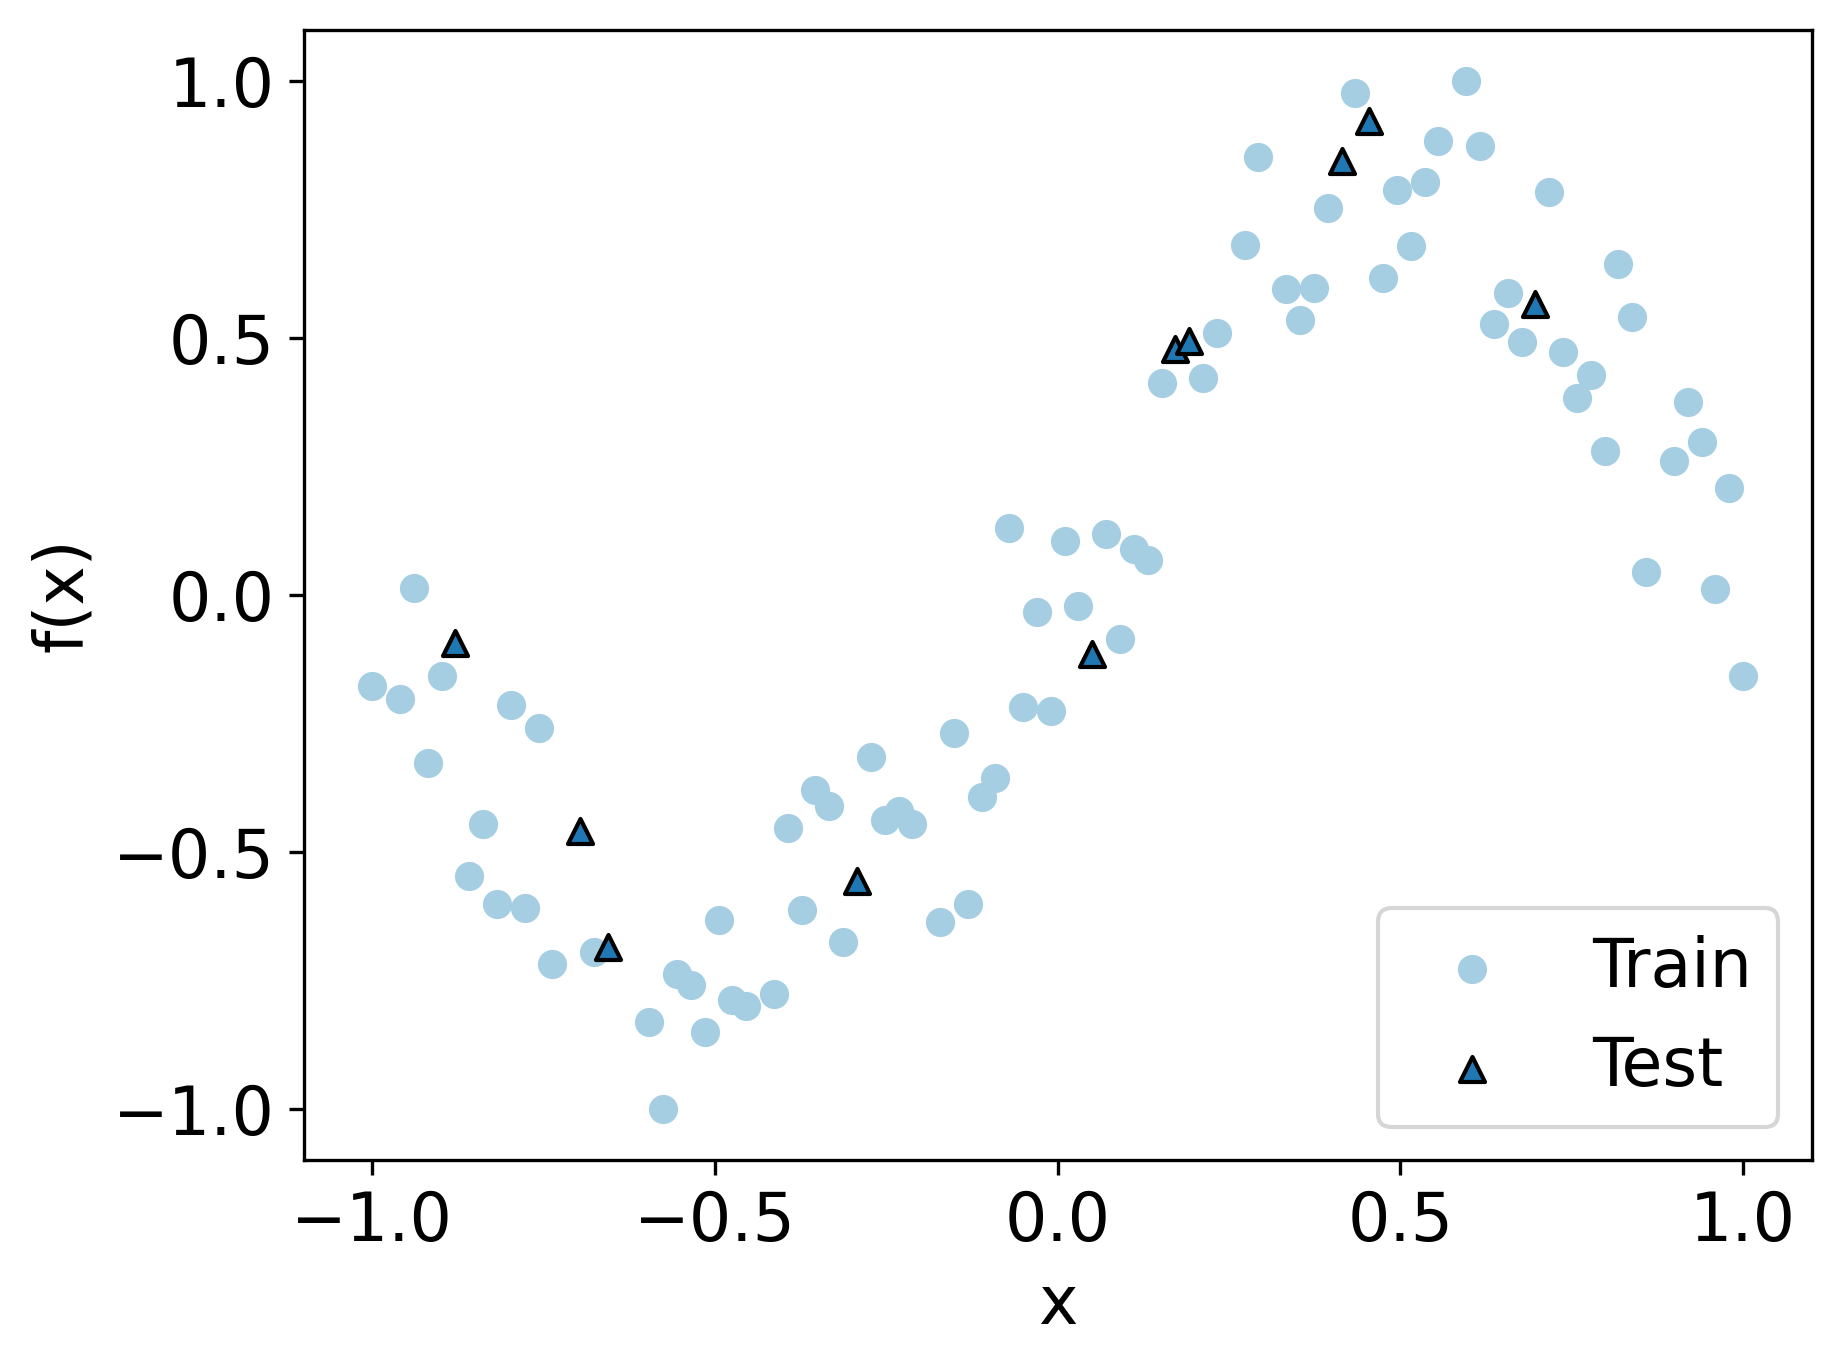
\includegraphics[width=\textwidth]{../images/Function_Fitting/function_dataset/sine_train_vs_test.png}
%		\caption{}
%		\label{fig:sine_train_vs_test}
%	\end{subfigure}
%	\caption{The function fitting dataset which consists of 90 total points, 80 for training and 10 used for testing, for the (a) linear, (b) quadratic, and (c) sine functions.}
%	\label{fig:train_vs_test}
%\end{figure}





Following model calibration using the function fitting dataset, we explore the appliciblity of PQCs for complex chemically relevant machine learning tasks.
The first chemically motivated dataset we explore is the BSE49 dataset, which contains the bond seperation energies (BSE)  for the homolytic bond cleavage of covalently bonded molecules, such as \ce{A-B -> A^{.} + B^{.}}.\cite{prasad_bse49_2021}
This dataset consists of 4394 datapoints, 1951 of which are existing and 2443 are hypthoetical structures, with 49 unique A-B single bond types.
In practice, we used 2436 of the hypothetical structures due to issues with valency exceptions when converting to RDKit mol objects which were later used for generating our features for the machine learning models.
An important aspect of machine learning in chemistry is the choice of molecular representation, or how the molecule is represented in the machine learning models.\cite{jones_molecular_2023}
Using RDKit\cite{noauthor_rdkit_nodate} we examined three commonly applied graph-based molecular preresentations, Molecular ACCess Systems (MACCS)\cite{durant_reoptimization_2002}, Morgan or extended-connectivity fingerprints \cite{morgan_generation_1965,rogers_extended-connectivity_2010}, and RDKit fingerprints.
All three of these methods are use traversals of the molecular graphs to encode various structural details into bit vectors.
Lastly, we explore both topology- and physics-based molecular representations, both of which encode the three-dimensional structure of molecules in various, unique ways.
Persistent images (PIs) are a topology-based fingerprint that uses persistence homology to encode topological information of three-dimensional molecular structures into fixed dimension images.\cite{adams_persistence_2017,townsend_representation_2020,schiff_augmenting_2022} 
We use the implementation from Townsend \textit{et al.}\cite{townsend_representation_2020}, which uses the Ripser Python package to generate PIs.\cite{tralie_ripserpy_2018}
Lastly, we explre two physics-based representations, Coulomb matrices (CMs) \cite{rupp_fast_2012} and smooth overlap of atomic positions (SOAPs), that were generated using DScribe.\cite{de_comparing_2016}
Due to the computational cost of computing the regularized entropy match (REMatch) kernel  with the SOAPs representation, we excluded this representation in the overall discussion.
We  also tested two different methods for representing the components of the bond separation chemical reaction, one where the feature vectors for the products are subtracted from the reactants, denoted by \textit{sub}, similar to the method used in Ref. \cite{garcia-andrade_barrier_2023}, and one that is composed of the reactant molecular only, denoted as \textit{AB}.


Since we are analyzing a diverse set of PQCs, we also examine a diverse set of classic regression models, with varying capabilities, such as ridge, lasso, elastic net, \textit{k}-nearest-neighbors, random forest, gradient boosting, support vector, kernel ridge, and gaussian process regression as implemented in sckit-learn.\cite{pedregosa_scikit-learn_2011}
Based on our results shown in Fig. \ref{fig:classical_molrepfig} we found that Morgan fingerprints
We found that the best molecular representation across all models test, as shown in Fig. \ref{fig:classical_molrepfig}, was Morgan fingerprints using the \textit{sub} formulation.
 
\begin{figure}[H]
	\centering	
	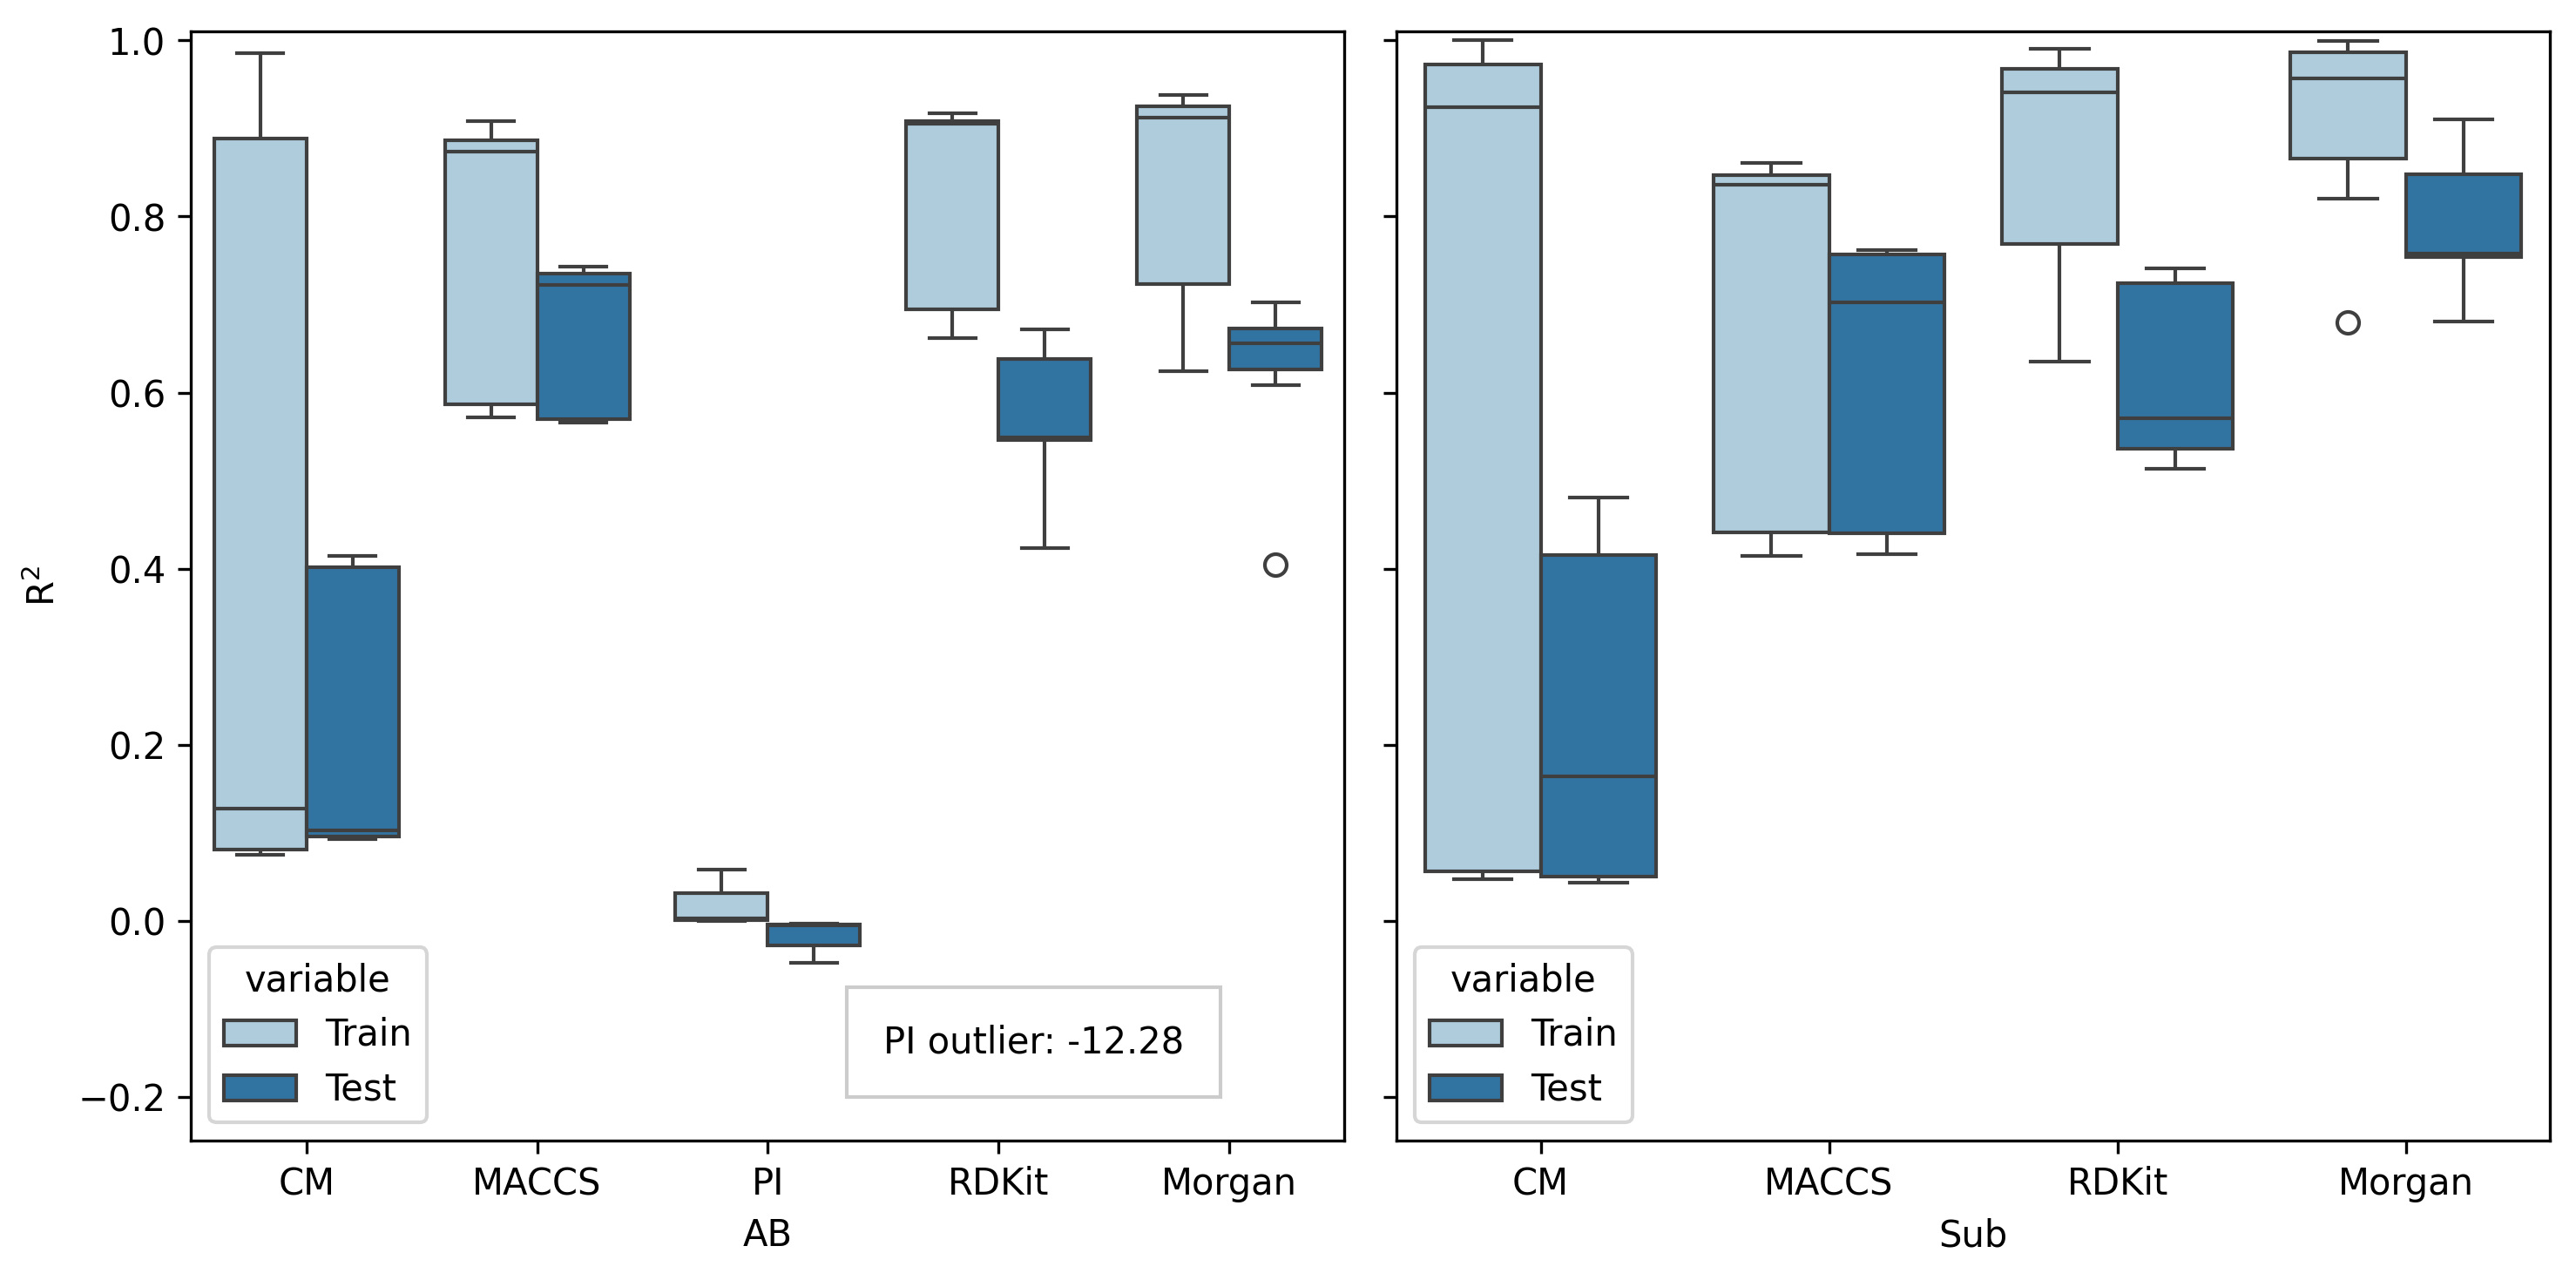
\includegraphics[width=\linewidth]{../images/BSE/classical/classical_molrepfig.png}
	\caption{Coulomb matrices (CMs), Molecular ACCess Systems (MACCS), persistence images (PIs), RDKit and Morgan fingerprints. Performance of a diverse set of molecular representations R$^{2}$}
	\label{fig:classical_molrepfig}
\end{figure}


An additional challenge of applying classical molecular representations for quantum machine learning models is mapping the classical features, often containing hundreds or thousands of features per sample, to the number of qubits used on the quantum device.
Initially, the Morgan fingerpints have 2048 features per sample, that need to be reduced down to 5 or 16 qubits.
We choose 5 and 16 qubits for two reasons, the first is that these were the standard number of qubits on IBM quantum devices when we started the project and the second is that reducing the number of features reduces the depth of the circuits.
To reduce the feature set from 2048 to 5 or 16 features, we explore two different methods, SHapley Additive ExPlanation analysis (SHAP)\cite{lundberg_unified_2017} and principal component analysis (PCA), as implemented in scikit-learn.\cite{pedregosa_scikit-learn_2011}
Figs. \ref{fig:BSE_classical_features_R2} and \ref{fig:BSE_bse_classical_features_MAE} show the results for the reductions using SHAP and PCA for the training and test set of using 5 and 16 features.
The initial model using 2048 features has a train and test mean absolute error (MAE) of 1.91 and 4.98 kcal/mol, with train and test R$^{2}$s of 0.99 and 0.91, respectively.
When using SHAP to reduce the feature set size to 5 features, we see that the training set has an MAE of 16.08 kcal/mol and an R$^{2}$ of 0.39, while for the test set has an MAE of 15.86 kcal/mol and an R$^{2}$ of 0.42.
When the number of features is reduced to 16 features using SHAP, we see slight improvements with train and test MAEs of 10.48 and 11.08 kcal/mol with R$^{2}$s of 0.69 and 0.68, respectively.
Using PCA, we see an improvement in accuracy for both 5 and 16 features, where the training sets have MAEs of 4.09 and 3.23 kcal/mol and the test sets have MAEs of 10.17 and 8.40 kcal/mol, respectively.
The R$^{2}$s for PCA with 5 and 16 features also shows improvement over the reductions using SHAP, with R$^{2}$s of 0.95 and 0.69 for the training and test set, respectively, using 5 features and 0.97 and 0.78 for the training and test set, respectively, using 16 features.
Due to the increased performance, despite exhibiting overfitting, we choose to use Morgan fingerprints reduced using PCA for our QML models.



\begin{figure}[H]
	\centering	
	\begin{subfigure}[b]{0.49\textwidth}
		\centering
		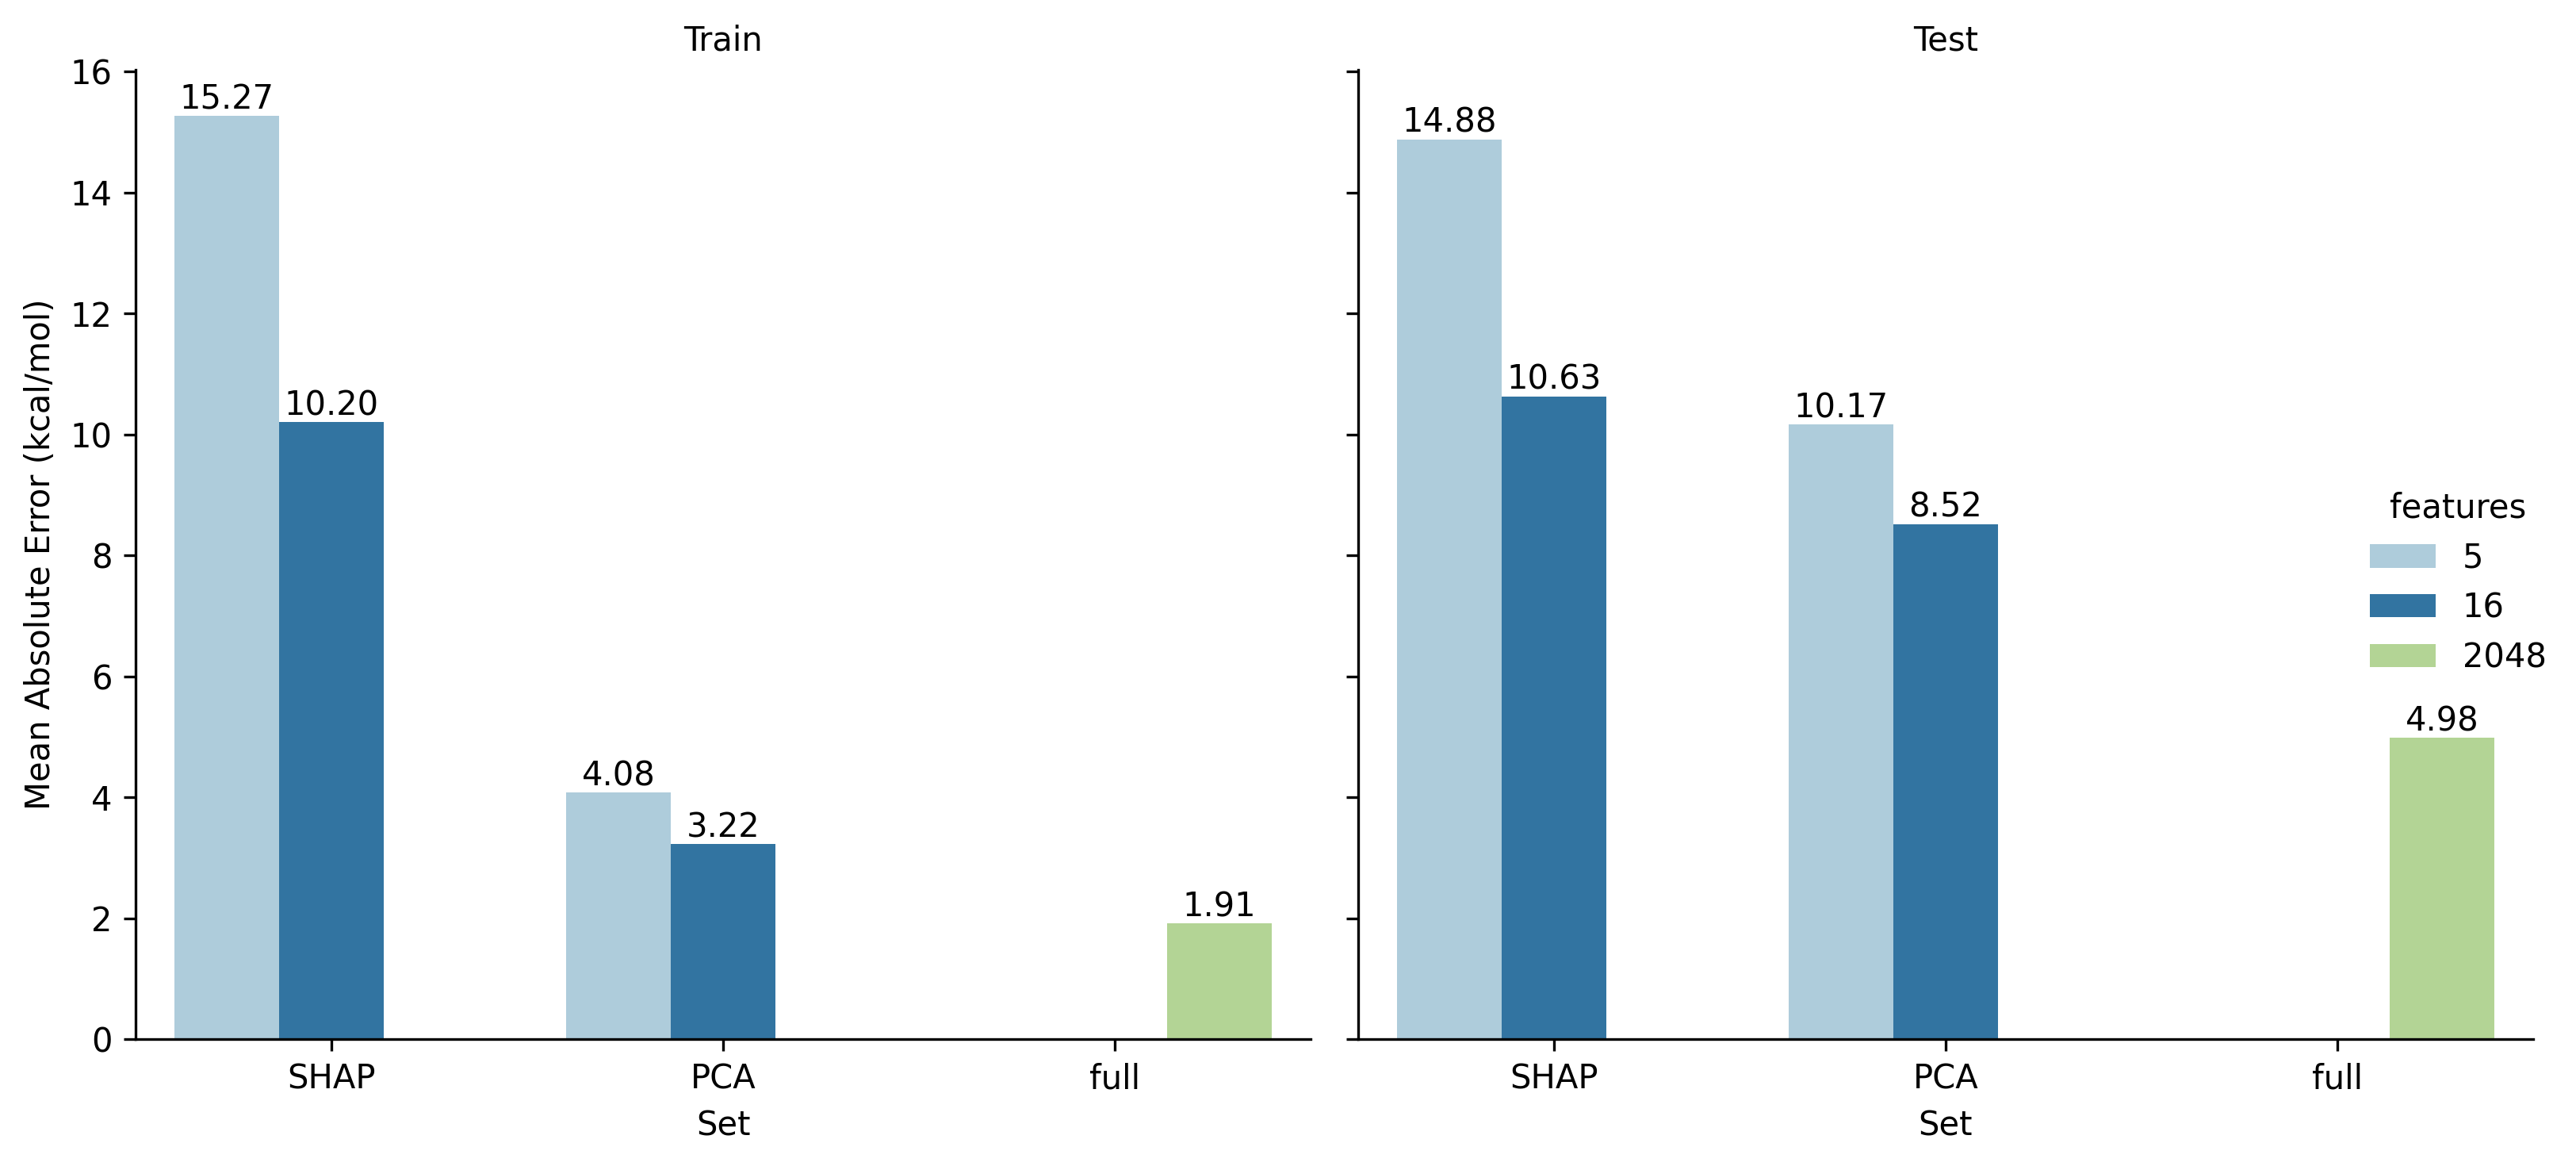
\includegraphics[width=\textwidth]{../images/BSE/classical_features_MAE.png}
		\caption{}
		\label{fig:BSE_bse_classical_features_MAE}
	\end{subfigure}
	\hfill		
	\begin{subfigure}[b]{0.49\textwidth}
		\centering
		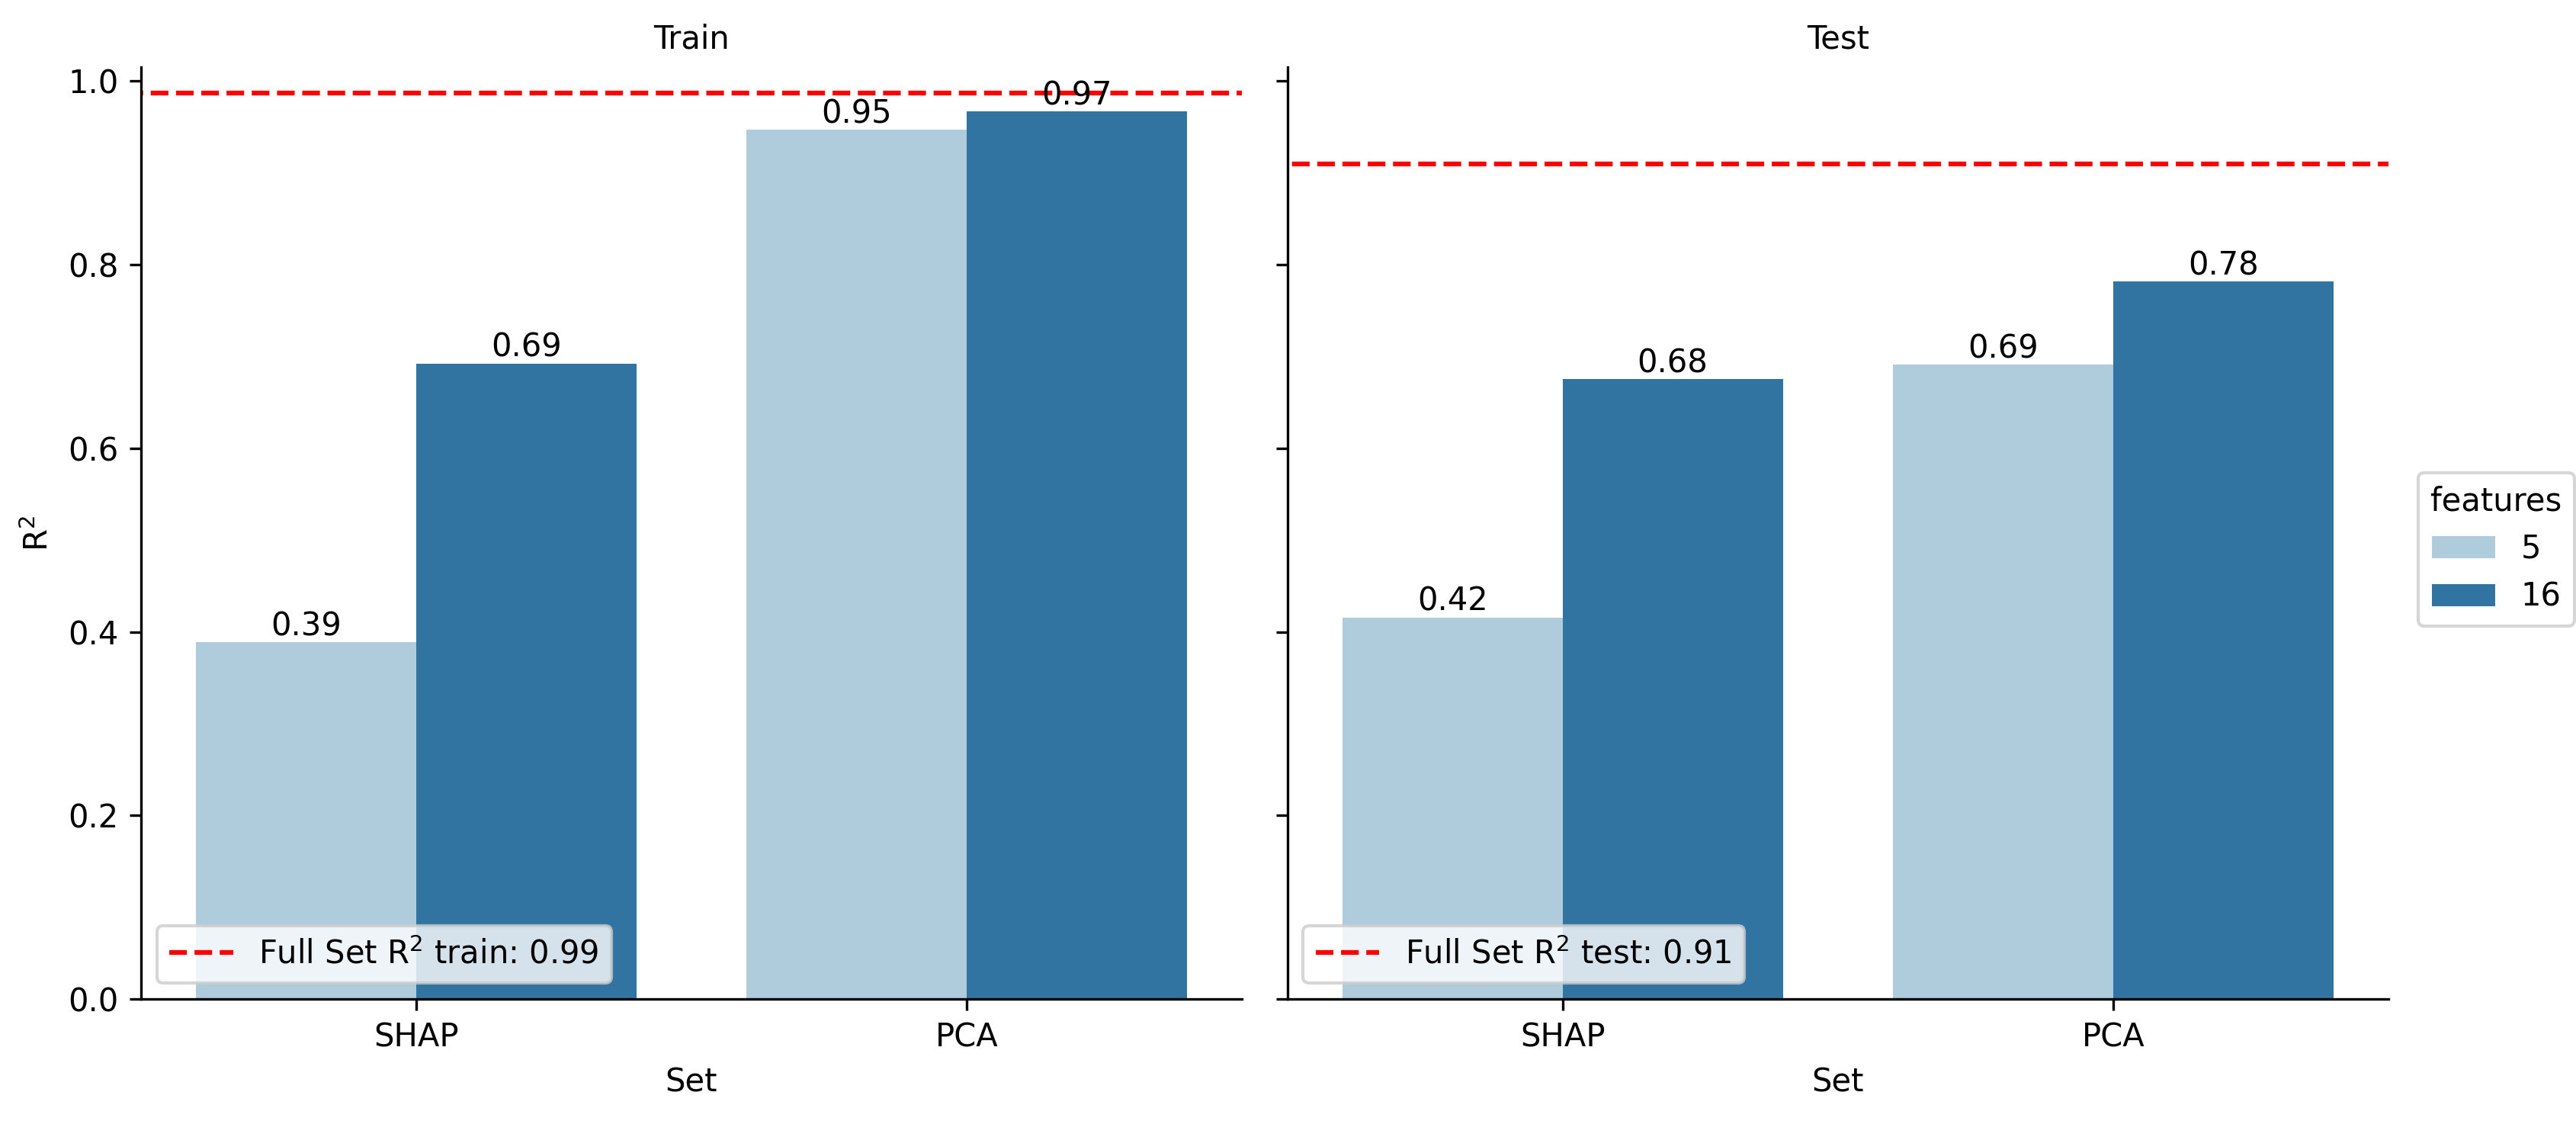
\includegraphics[width=\textwidth]{../images/BSE/classical_features_R2.png}
		\caption{}
		\label{fig:BSE_classical_features_R2}
	\end{subfigure}
	\caption{Feature reduction of the BSE dataset represented using }
	\label{fig:bse_classical_features}
\end{figure}


The next chemical dataset explored is based on the data-driven coupled-cluster (DDCC) method, which is a machine learning-based approach for accelerating the convergence of coupled-cluster singles and doubles (CCSD) calculations.\cite{townsend_data-driven_2019,jones_chapter_2023}
This method works by predicting the $t_{2}$-amplitudes of the CCSD wave function (Eq. \ref{eq:cc_wfn}) with features generated using lower-level methods, such as Hartree-Fock (HF) and M{\o}ller-Plesset second-order perturbation theory (MP2), which are used to initialize CCSD calculations.

The coupled-cluster wave function takes the general form,
\begin{equation}
	\ket{\Psi_{\text{CC}}} = \exp(\hat{T}) \ket{\Psi_{0}}
	\label{eq:cc_wfn}
\end{equation}
where the cluster operator is denoted as $\hat{T}$ and the reference, Hartree-Fock wave function is denoted as $\ket{\Psi_{0}}$.
The CCSD wave function truncates the cluster operator to only include singles and doubles excitations.
The CCSD correlation energy is defined as,
\begin{equation}
	E^{\text{CCSD}}_{\text{corr}} = \sum_{\substack{a<b \\ i<j}} \mel{ij}{}{ab} t^{ab}_{ij} + \sum_{\substack{a<b \\ i<j}} \mel{ij}{}{ab} t^{a}_{i} t^{b}_{j}
	\label{eq:cc_corr}
\end{equation}
where $i$ and $j$ denote occupied orbitals, $a$ and $b$ denote virtual orbitals, $t^{ab}_{ij}$ are the $t_{2}$-amplitudes which correspond to two-electron excitations, 
$t^{a}_{i}$ and $t^{b}_{j}$ are $t_{1}$-amplitudes corresponding to one-electron excitations, and $\mel{ij}{}{ab}$ are two-electron integrals.

For each two-electron excitation, $t^{ab}_{ij}$, a feature set can be generated from HF and MP2.
The feature set includes the MP2 $t_{2}$-amplitudes, which are used to initialize the CCSD amplitudes,
\begin{equation}
	t^{ab}_{ij(\text{MP2})} = \frac{\mel{ij}{}{ab}}{\varepsilon_{i}+\varepsilon_{j}-\varepsilon_{a}-\varepsilon_{b}}
	\label{eq:MP2_t2}
\end{equation}
where $\varepsilon_{i}$ and $\varepsilon_{j}$ denote the orbital energies of the occupied orbitals $i$ and $j$, while the virtual orbitals $a$ and $b$ are denoted by $\varepsilon_{a}$ and $\varepsilon_{b}$.
Features related to the MP2 $t_{2}$-amplitudes that are also included in the feature set are the numerator ($\mel{ij}{}{ab}$) and denominator ($\varepsilon_{i}+\varepsilon_{j}-\varepsilon_{a}-\varepsilon_{b}$), a binary feature to denote whether the excitation goes to the same virtual orbital, and the orbital energies ($\varepsilon_{i},\varepsilon_{j},\varepsilon_{a},\varepsilon_{b}$).
The feature set also includes terms related to the individual contributes to the orbital energies are also included, such as the one-electron Hamiltonain ($h$), Coulombic matrix ($J$), and exchange matrix $K$, and Coulombic and exchange integrals ($J^{i}_{a},J^{j}_{b},K^{a}_{i},K^{b}_{j}$).
In total, there are 30 features for each $t_{2}$-amplitude due to the addition of features that denote the sign and magntudes of the previously mentioned features.

Our dataset consists of 199 water molecules from the study by Townsend and Vogiatzis using the STO-3G basis set\cite{hehre_selfconsistent_1970} and frozen core orbitals.
All data was generated using Psi4\cite{parrish_psi4_2017} and Psi4Numpy\cite{smith_psi4numpy_2018}.
As previously mentioned, the DDCC method is data intensive regarding the number of samples per molecule, for example, each water molecule has 4 occupied and 2 virtual orbitals.
The number of $t_{2}$-amplitudes is equivalent to $(N_{occ})^{2}(N_{virt})^{2}$, where $N_{occ}$ denotes the number of occupied orbitals and $N_{virt}$ denotes the number of virtual orbitals, so the total number of $t_{2}$-amplitudes per molecule is 64.
Further details regarding the feature set and implementation can be found in \cite{townsend_data-driven_2019}

Like the BSE dataset, the 30 features from the full DDCC feature set must be reduced to 5 or 16 features using SHAP or PCA.
Unlike the BSE dataset, we choose SHAP over PCA for the feature reduction since there is a direct correlation between the input features and output values.
As shown in Fig. \ref{fig:DDCC_feature_set}, 5 and 16 features can accurately recover performance of the original model using 30 features, where all three models have train and test R$^{2}$s of 1.00.
Due to the computational costs of running QML models, we will then use only 5 features for all DDCC QML models.
The 5 most important features are the two-electron integrals ($\mel{ij}{}{ab}$), MP2 $t_{2}$-amplitudes ($t^{ab}_{ij(\text{MP2})}$), the magnitude of the MP2 $t_{2}$-amplitudes, and the difference in orbital energies ($\varepsilon_{i}+\varepsilon_{j}-\varepsilon_{a}-\varepsilon_{b}$).



\begin{figure}[H]
	\centering
	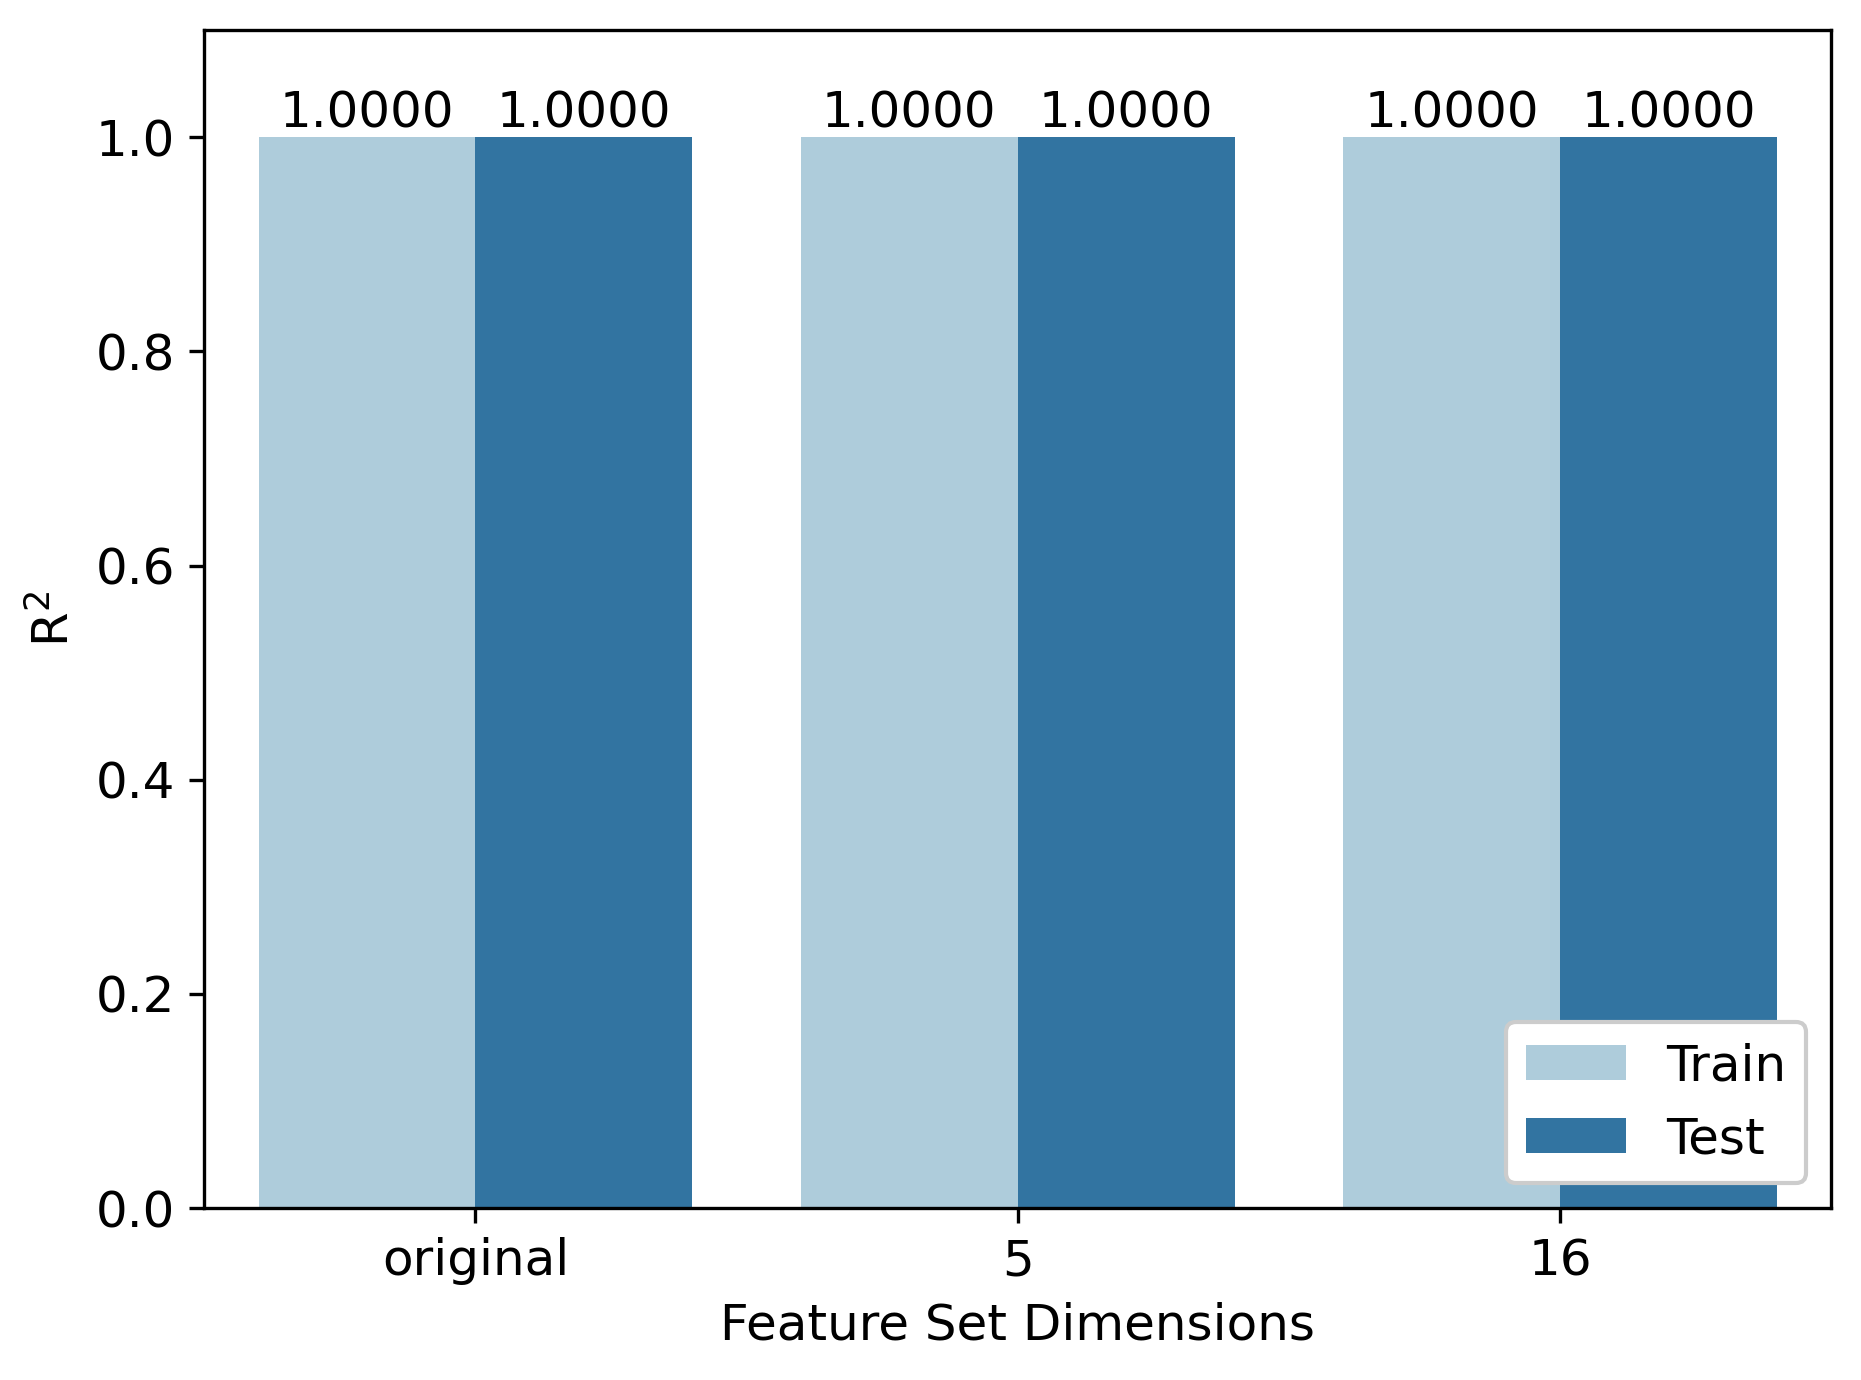
\includegraphics[width=0.49\textwidth]{../images/DDCC/DDCC_feature_set.png}
	\caption{}
	\label{fig:DDCC_feature_set}
\end{figure}


% Make distribution plot
%\begin{figure}[H]
%	\centering
%	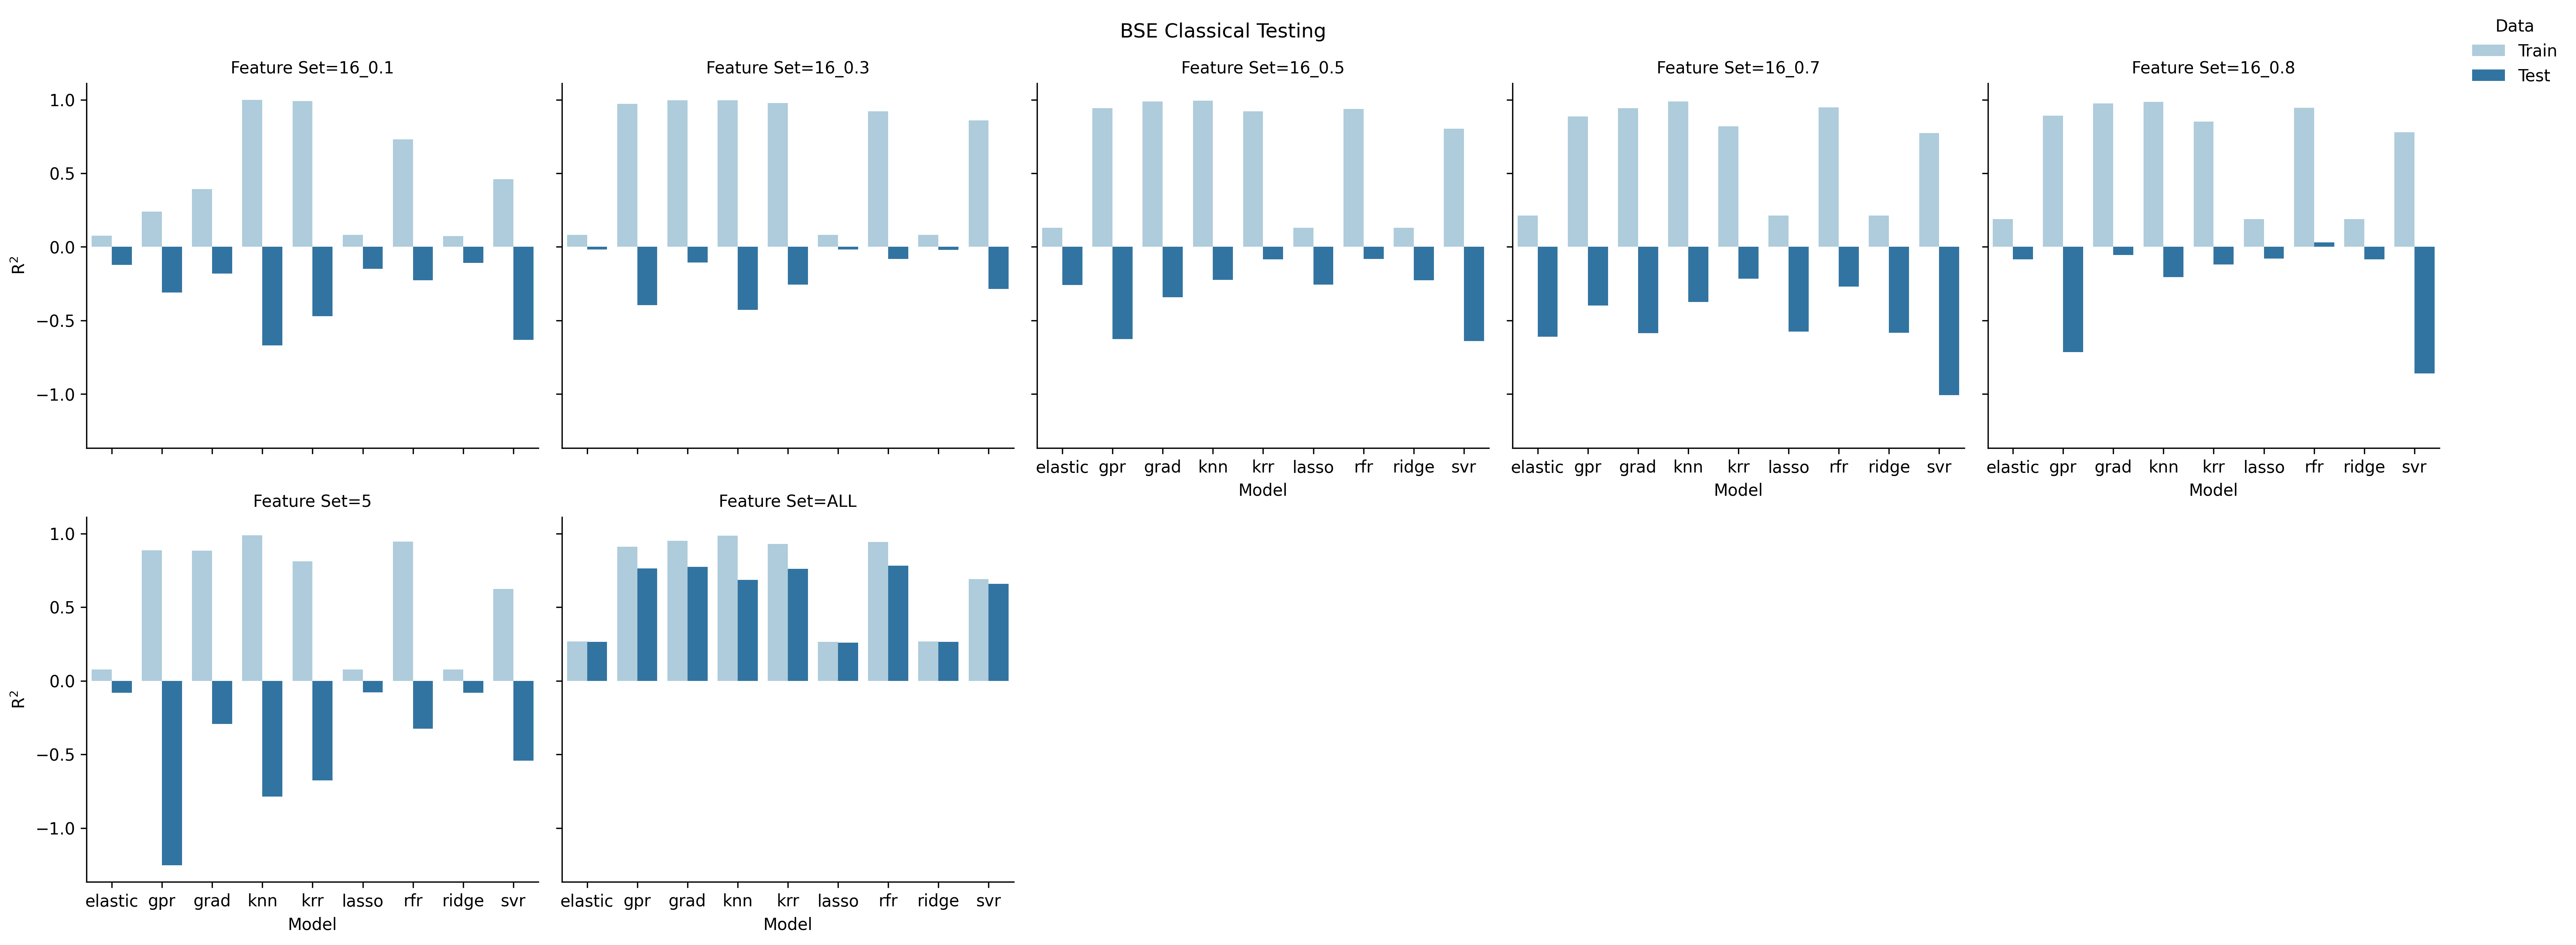
\includegraphics[width=\linewidth]{../images/BSE.png}
%	\caption{BSE}
%	\label{fig:BSE}
%\end{figure}







\section{Results and Discussion}
\label{section:results_and_discussion}

\subsection{Function Fitting}
To calibrate the PQCs, we perform an initial study of the 168 encoder-ansatz pairs using both 5 and 16 qubits.
Individual heat maps showing the performance of the encoder-ansatz pairs and box plots showing the overall statistics for each encoder and ansatz are shown for the 5 and 16 qubit models in SI Section \siref{section:si_functionfitting}.


Starting with the five qubit function fitting, we found that out of the
168 encoder-ansatz pairs, for the linear function (SI Fig. \siref{fig:linear_heatplots}) is is A1\_ESU2 with a train and test R$^{2}$ of 0.9886 and 0.9893, respectively.
Box plots for the encoders (left) and variational layers (right) are shown in SI  Fig. \siref{fig:linear_boxplots}, where, the best encoder is IQP, with a mean R$^{2}$ of 0.8434, and best ansatz layer Full-CRX, with a mean R$^{2}$ of 0.7562.
For the quadratic function, the best encoder-ansatz pair is A1-A1-CNOT\_Full-CRX with a train and test R$^{2}$ of 0.8809 and 0.7309, respectively, as shown in SI Fig \siref{fig:quadratic_heatplots}.
On average the best encoder is A1-A1-CNOT with an R$^{2}$ of 0.5541 and best variational layer is Full-CRX with an R$^{2}$ of 0.5958 (SI  Fig. \siref{fig:quadratic_boxplots}).
For the sine function, SI  Fig. \siref{fig:sine_heatplots}, M-M-CZ\_Full-CRX is the best encoder-ansatz pair with a train and test R$^{2}$ of 0.8887 and 0.9081, respectively.
As shown in SI  Fig. \siref{fig:sine_boxplots}, the best encoder is M with an average R$^{2}$ of 0.6456 and best variational layer is Full-CRX with a mean R$^{2}$ of 0.7551.
Across all three five qubit function fitting datasets, on average, the best encoders are M-A2-CZ with an average R$^{2}$ of 0.4776 (Fig. \ref{fig:five_feature_function_fitting_boxplots} left) and ansatz is Full-CRX with an average R$^{2}$ of 0.7023 (Fig. \ref{fig:five_feature_function_fitting_boxplots} right).

For the sixteen qubit function fitting evaluation of the 168 encoder-ansatz pairs, we found that, similarly to the five qubit data, for the linear function the best pair is A1\_ESU2 with train and test R$^{2}$s of 0.9886 and 0.9893, respectively, as highlighted in SI Fig. \siref{fig:sixteenlinear_heatplots}.
Like the five qubit data, the best encoder is also IQP with an average R$^{2}$ of 0.7800 (SI Fig. \siref{fig:sixteenlinear_boxplots} left), while the best ansatz varies from the five qubit data, Full-Pauli-CRZ with a mean R$^{2}$ of 0.3947 (SI Fig. \siref{fig:sixteenlinear_boxplots} right).
The A1-A1-CZ\_Modified-Pauli-CRX encoder-ansatz pair has the best overall model performance, highlighted in SI Fig. \siref{fig:sixteenquadratic_heatplots}, where the training set has an R$^{2}$ of 0.8415 and the test set has an R$^{2}$ of  0.7722.
As demonstrated in SI Fig. \siref{fig:sixteenquadratic_boxplots}, the best encoders and ans\"{a}tze are A1-A1-CNOT and Full-Pauli-CRX, with mean R$^{2}$s of 0.5759 and 0.4474, respectively.
For the last sixteen qubit dataset, the sine function data (SI Fig. \siref{fig:sixteensine_heatplots}), the best encoder-ansatz pair is A1-A1-CZ\_Full-Pauli-CRZ	with an R$^{2}$ of 0.8147 for the training set and an R$^{2}$ of 0.8626	for the test set.
SI Fig. \siref{fig:sixteensine_boxplots} highlights that the best encoder is M with a mean R$^{2}$ of 0.5824 and best ansatz, on average, is Full-Pauli-CRZ with an R$^{2}$ of 0.4881.
Across all three function fitting datasets, the sixteen qubit data varies where the best encoders are IQP with an average R$^{2}$ of 0.4506 and ans\"{a}tze is Full-Pauli-CRZ with an average R$^{2}$ of 0.4393.

\begin{figure}[H]
	\centering
	\begin{subfigure}[b]{0.49\textwidth}
		\centering
		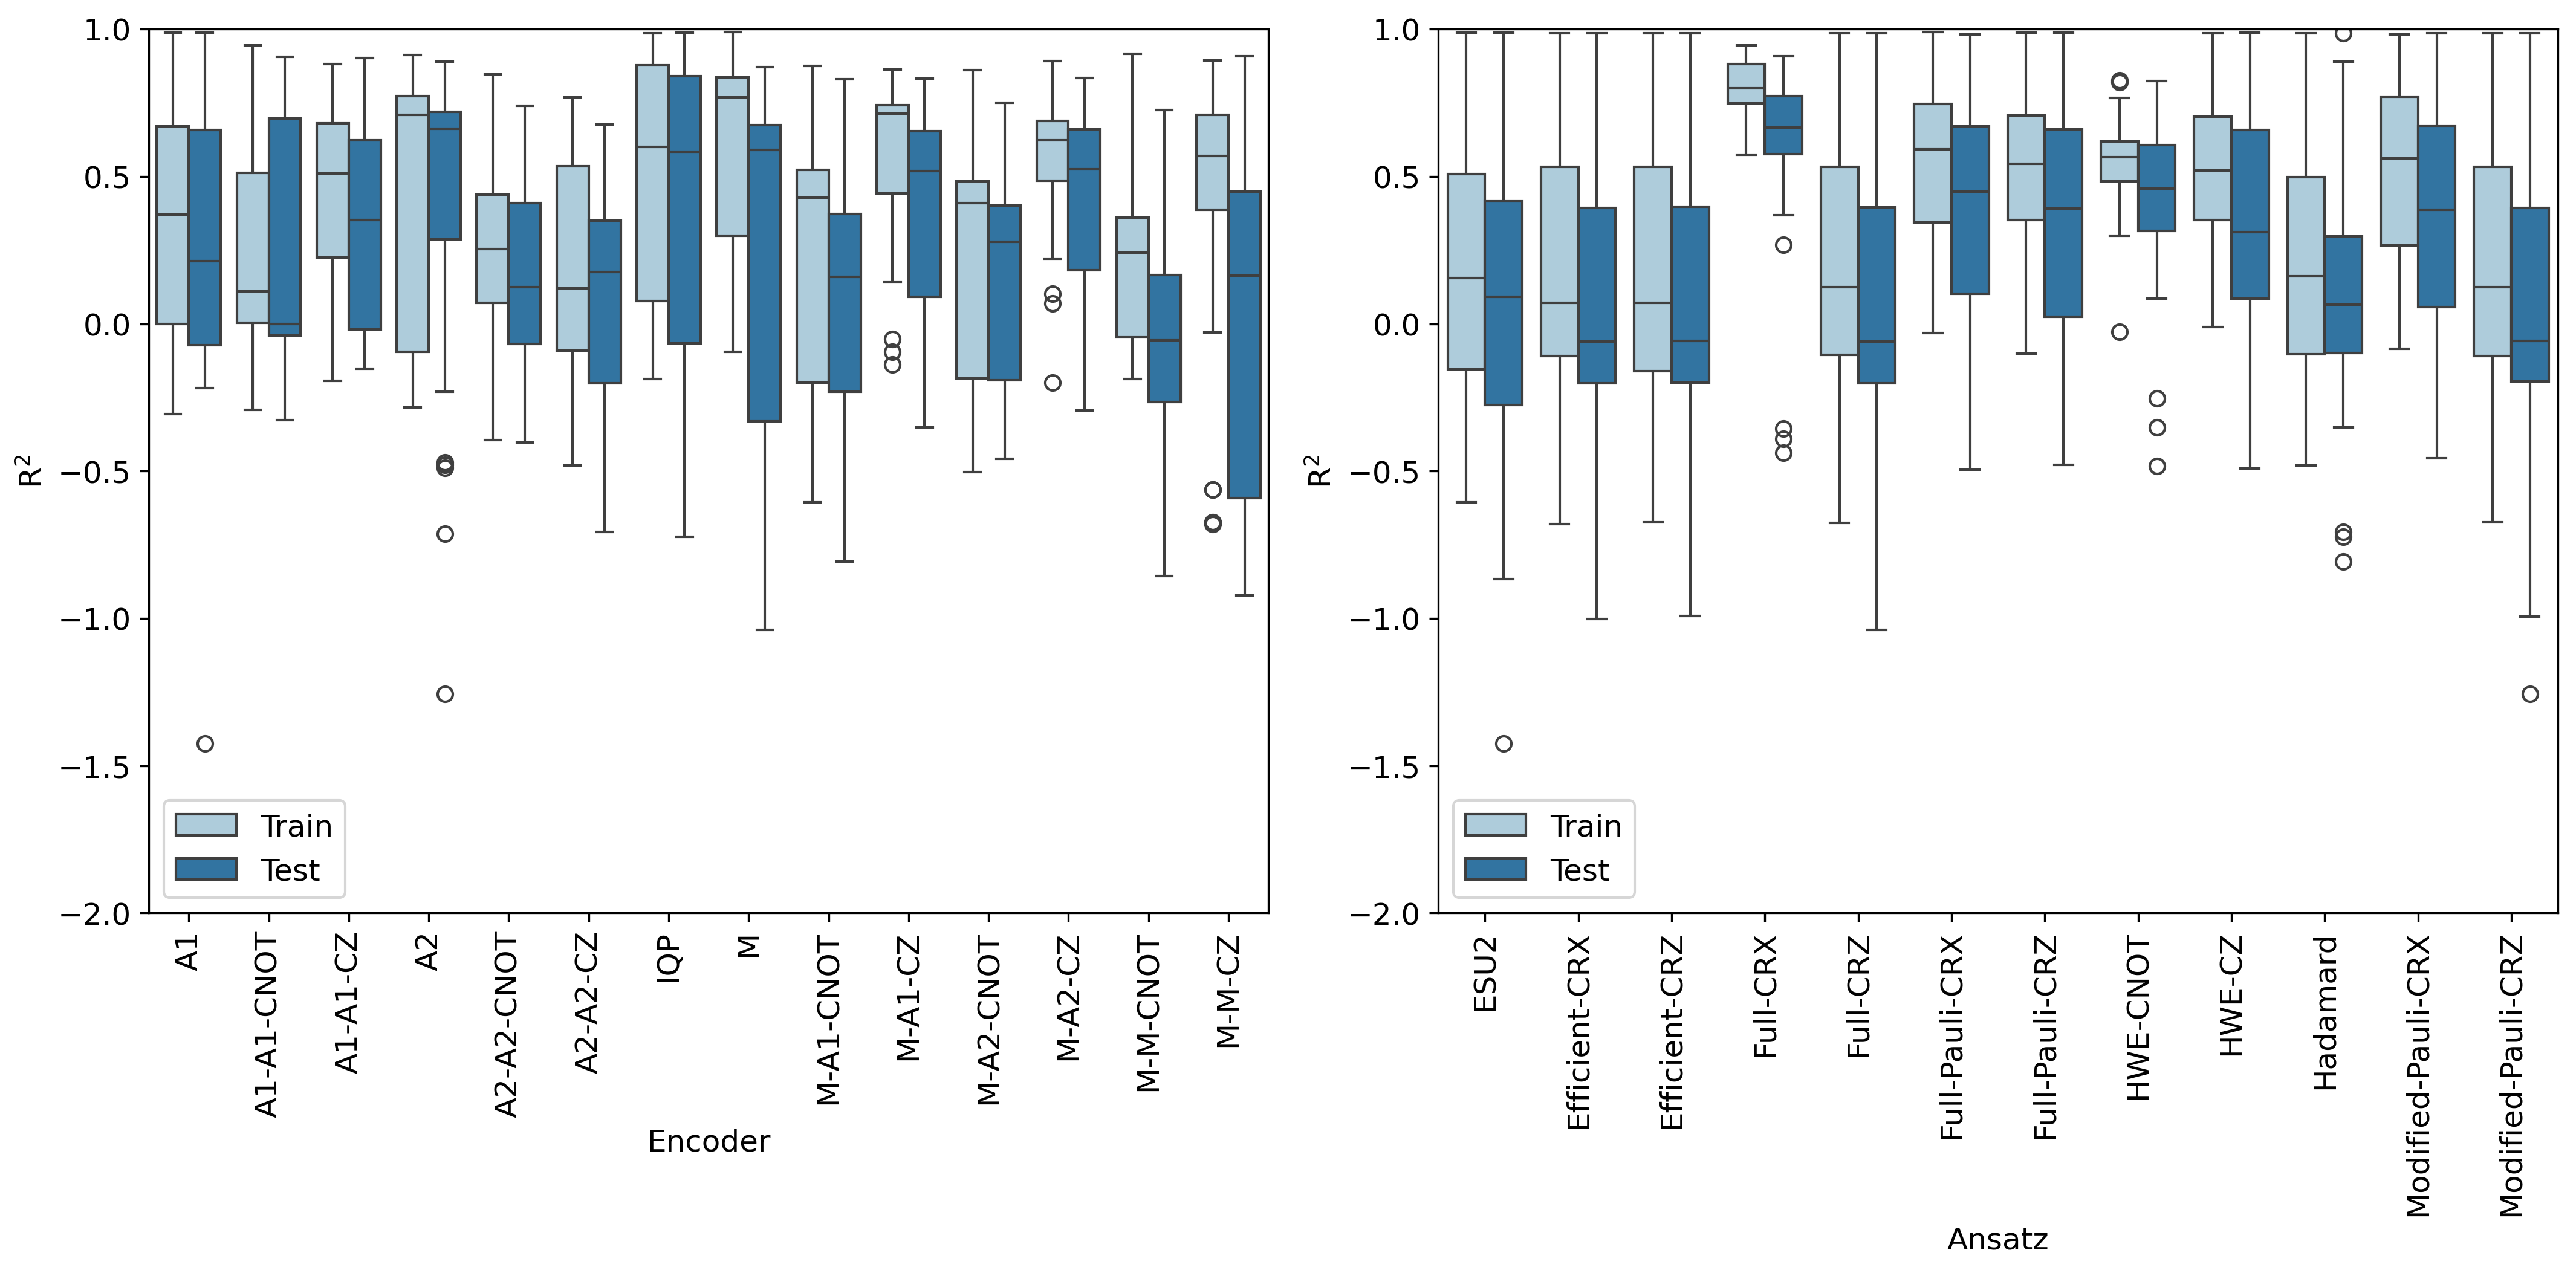
\includegraphics[width=\textwidth]{../images/Function_Fitting/fivequbit/five_feature_function_fitting_boxplots.png}
		\caption{}
		\label{fig:five_feature_function_fitting_boxplots}
	\end{subfigure}
	\hfill		
	\begin{subfigure}[b]{0.49\textwidth}
		\centering
		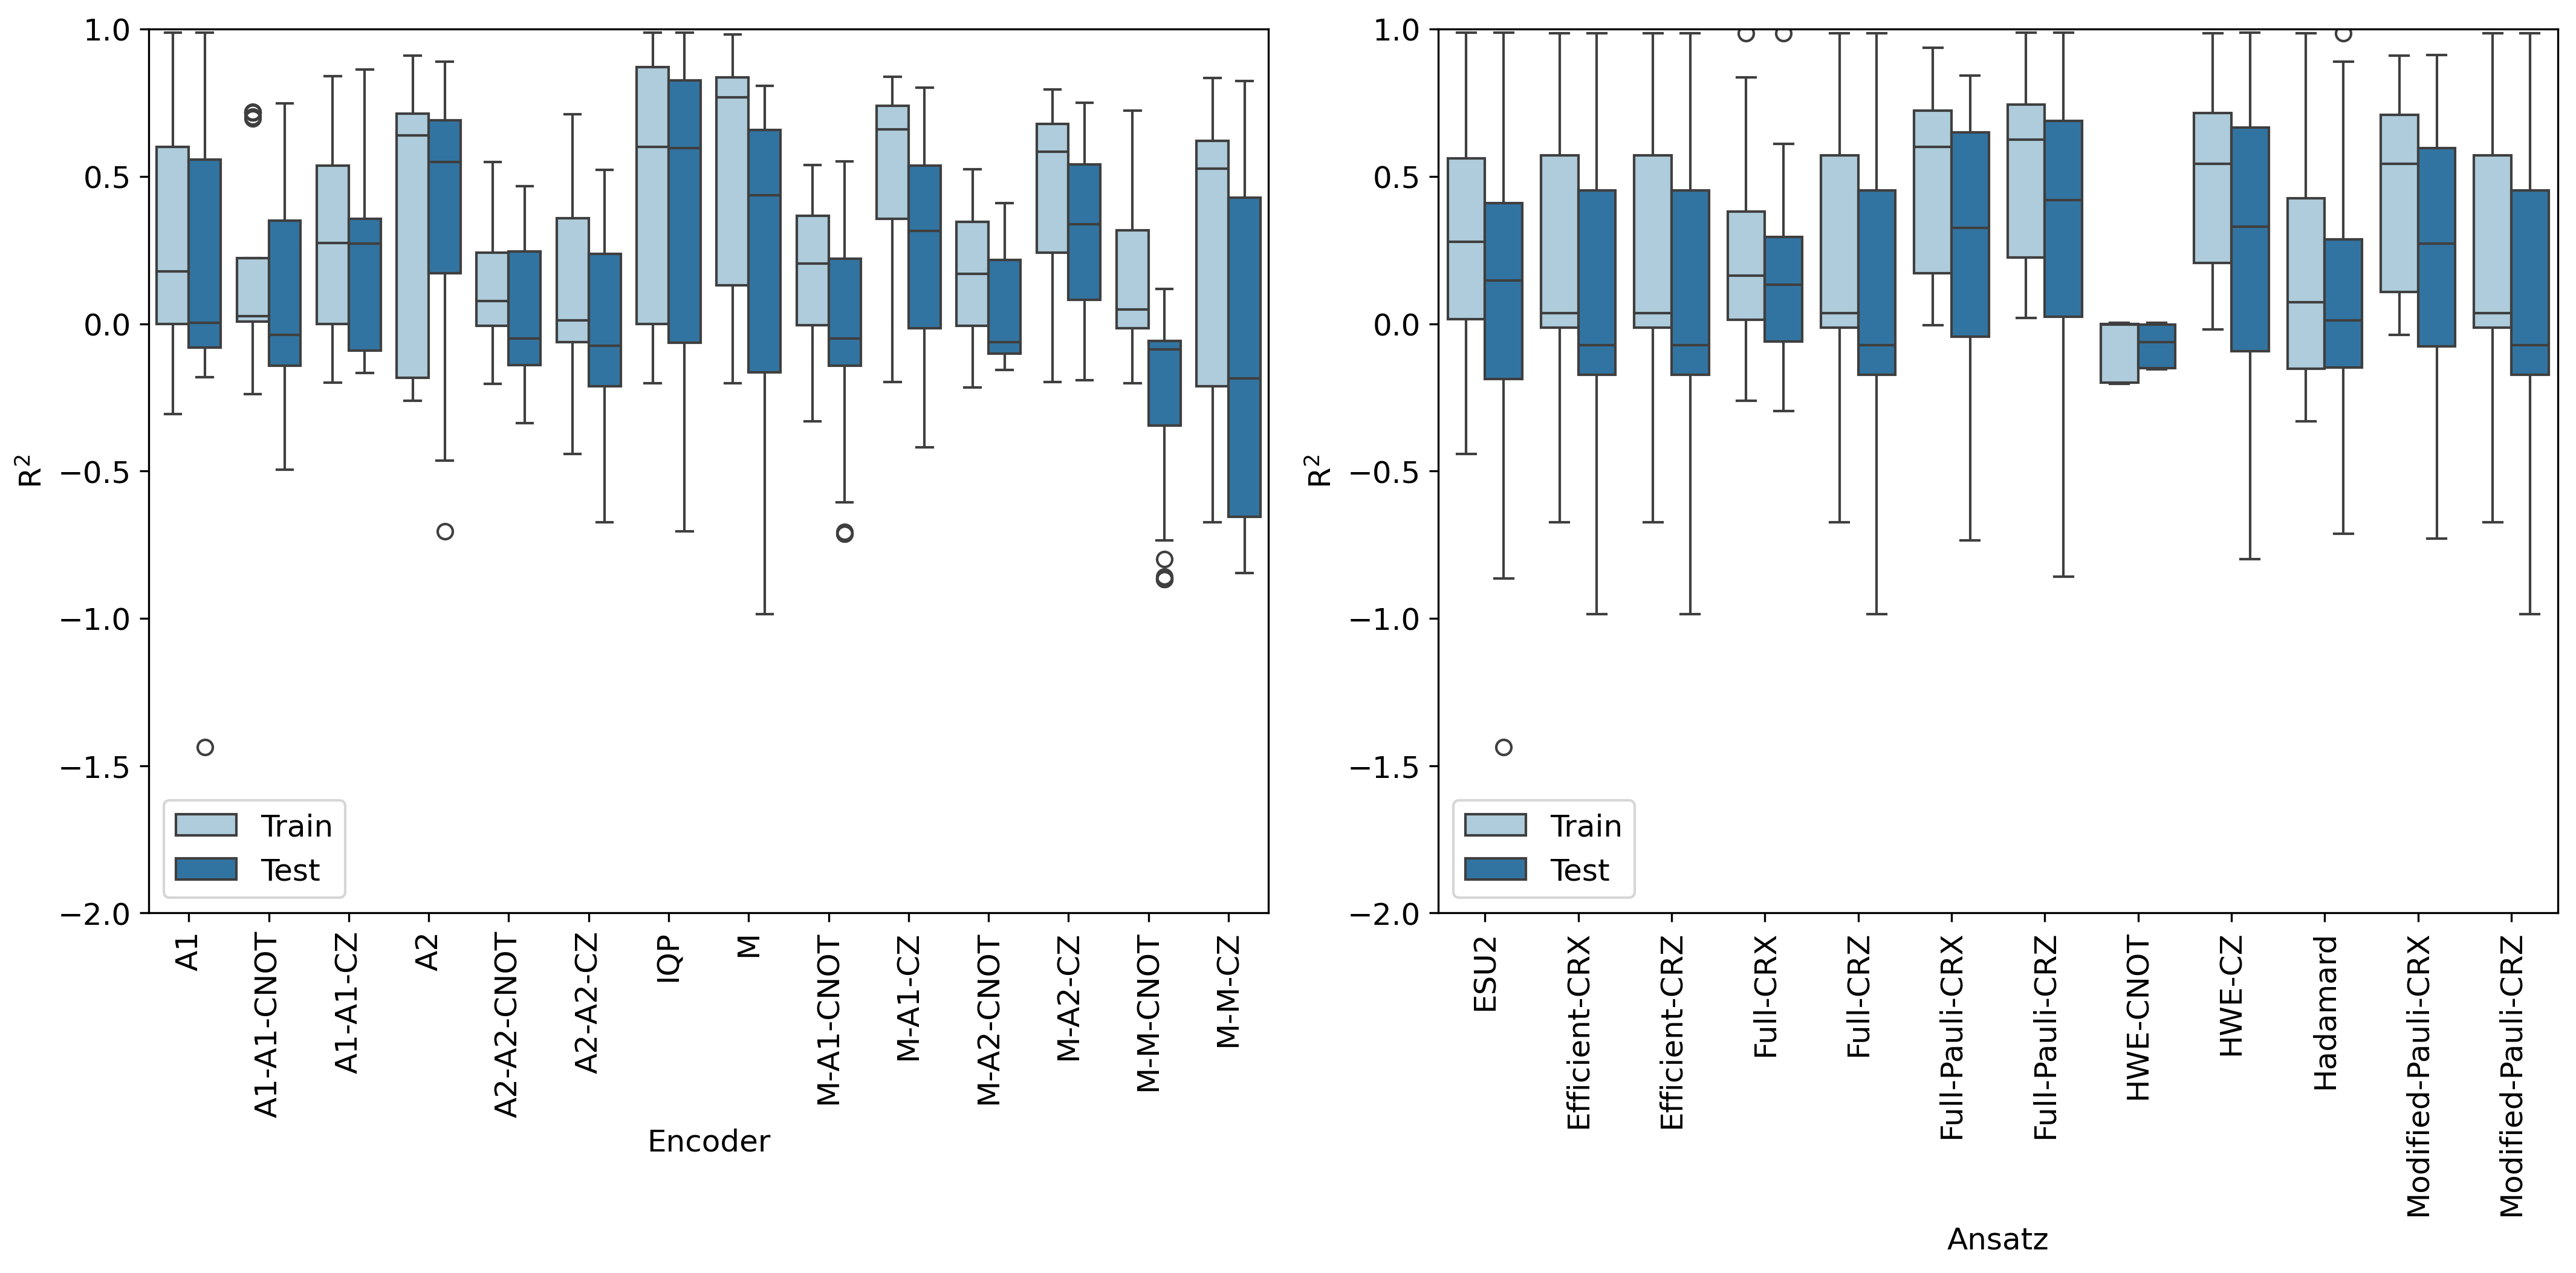
\includegraphics[width=\textwidth]{../images/Function_Fitting/sixteenqubit/sixteen_feature_function_fitting_boxplots.png}
		\caption{}
		\label{fig:sixteen_feature_function_fitting_boxplots}
	\end{subfigure}
	\hfill		
	\caption{The combined performance of all three function fitting datasets for both the (a) five and (b) sixteen qubit models is evaluated using the R$^{2}$ (y-axis) versus the encoders (left) and ans\"{a}tze (right).}
	\label{fig:function_fitting_boxplots}
\end{figure}


Following the initially analysis of the performance of the 168 PQCs using both five and sixteen qubits, we experimented with the effect of the re-upload depth (RUD) and number of ansatz layers (AL) using the sixteen qubit circuits.
We chose to use the sixteen qubit circuits over the five qubit circuits since these circuits have complexity more similar to when the circuits are used for the chemical dataset in terms of the number of parameters and optimization times.
From the initial 168 PQCs, for each function fitting dataset, we choose the five best (top row), five median (middle row), and five worst (bottom row) circuits to see the effects of increasing the RUD and AL on model performance as shown in Figs. \ref{fig:16qubit_Linear_RUD_AL}, \ref{fig:16qubit_Quadratic_RUD_AL}, and  \ref{fig:16qubit_Sine_RUD_AL}.
For the linear (Fig. \ref{fig:16qubit_Linear_RUD_AL}), quadratic (\ref{fig:16qubit_Quadratic_RUD_AL}), and sine (Fig. \ref{fig:16qubit_Sine_RUD_AL}) data, some generalities arise for the five best circuits. 
We see that for these circuits, increasing the number of AL from 1 to 3 or 5 improves model performance more than RUD.
For the median performers, the RUD improves model performance more than the ansatz layers.
And lastly, for the worse performers a general trend does not exist and increasing the RUD and AL depends on the dataset and circuit architecture. 


% Commented this out because it is not useful for the overall discussion
%While an increase in the circuit depth, either by increasing the RUD or AL, is associated with an increase in model performance this is also associated with an increased computational cost. 
%In Figs. \ref{fig:linear_circuitdepth_vs_R2}, \ref{fig:quadratic_circuitdepth_vs_R2}, and \ref{fig:sine_circuitdepth_vs_R2} we  highlight this trade-off, where the x-axes denote circuit depth, y-axis denotes the R$^{2}$, and the median train and test R$^{2}$ are shown in red and blue, respectively, for all 15 circuits. 
Despite these trends, we found that for the linear function, the best performing model is IQP\_Full-Pauli-CRZ  with a RUD and AL of 1.
This circuit also has a training and test R$^{2}$ of 0.9883 and 0.9891, respectively, and a depth of 95.
Unlike the best linear circuit, the best circuits for both the quadratic and sine data, IQP\_Full-Pauli-CRX	 and A2\_HWE-CZ, respectively,  benefit from an increased RUD, with the best models having a RUD of 5 and AL of 1.
These two circuits differ in depth and performance, with the IQP\_Full-Pauli-CRX for the quadratic data having a circuit depth of 520, training R$^{2}$ of 0.9817, and test R$^{2}$ of 0.9609 and the A2\_HWE-CZ circuit for the sine data having a depth of 105 , training R$^{2}$ of 0.9156, and test R$^{2}$ of 0.9576.
Following these insights, we applied these circuits for analyzing the effects of the training set size on model performance using learning curves and the effects of error mitigation using noisy simulation.


\begin{figure}[H]
	\centering	
	\begin{subfigure}[b]{0.49\textwidth}
		\centering
		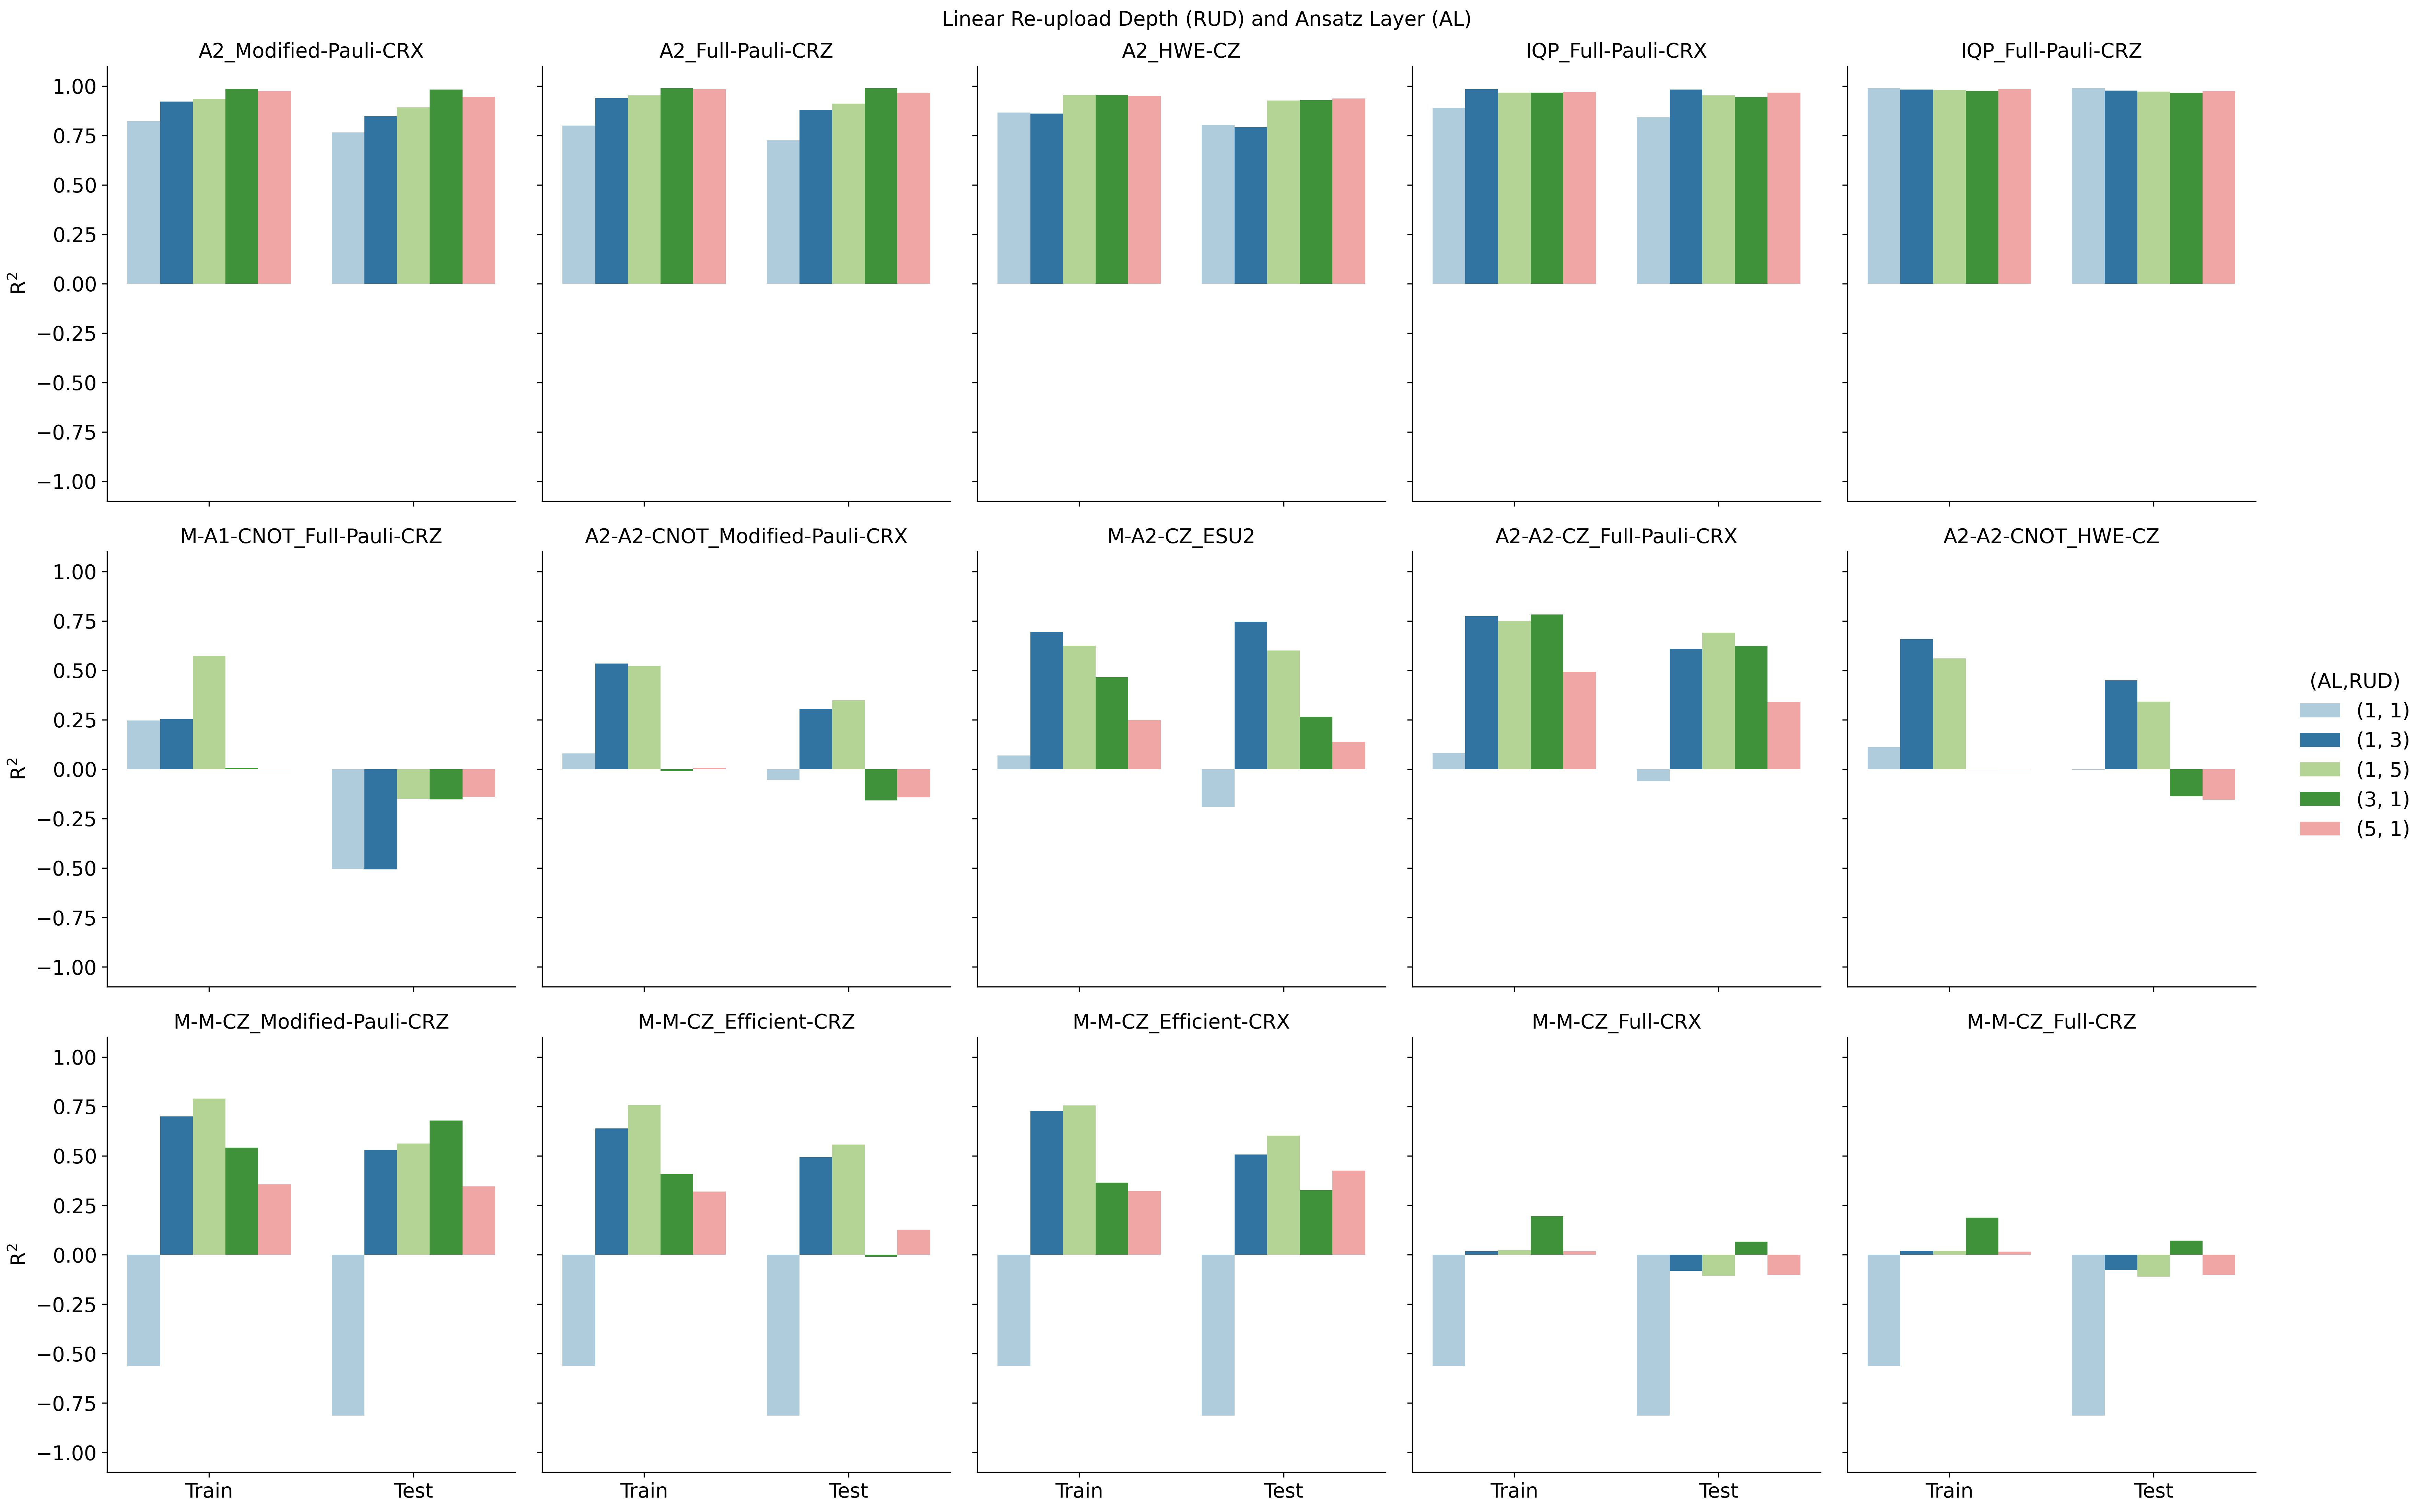
\includegraphics[width=\linewidth]{../images/Function_Fitting/sixteenqubit/16qubit_Linear_RUD_AL}
		\caption{}
		\label{fig:16qubit_Linear_RUD_AL}
	\end{subfigure}
	\hfill	
%	\begin{subfigure}[b]{0.49\textwidth}
%		\centering
%		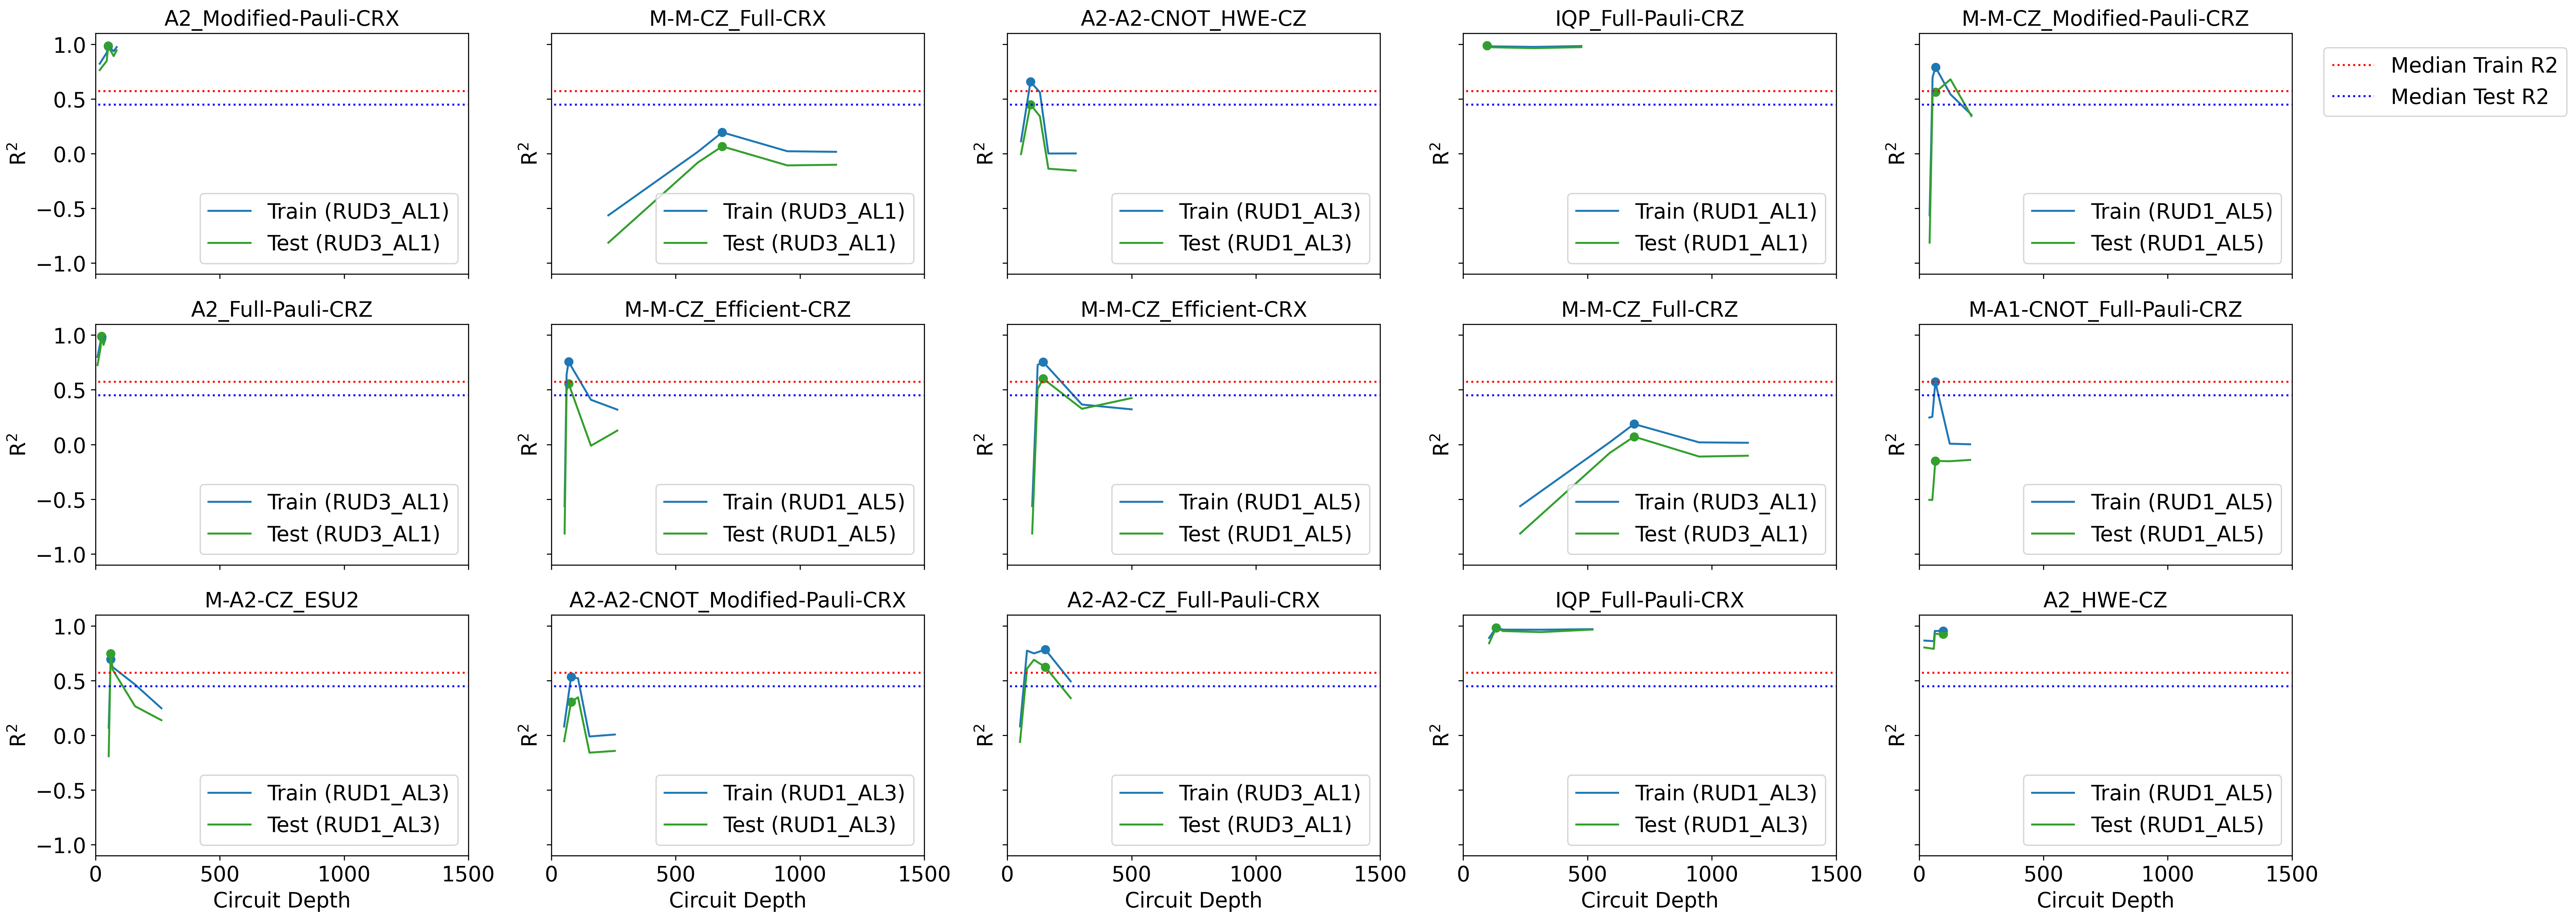
\includegraphics[width=\linewidth]{../images/Function_Fitting/linear_circuitdepth_vs_R2}
%		\caption{}
%		\label{fig:linear_circuitdepth_vs_R2}
%	\end{subfigure}
%	\hfill		
	\begin{subfigure}[b]{0.49\textwidth}
		\centering
		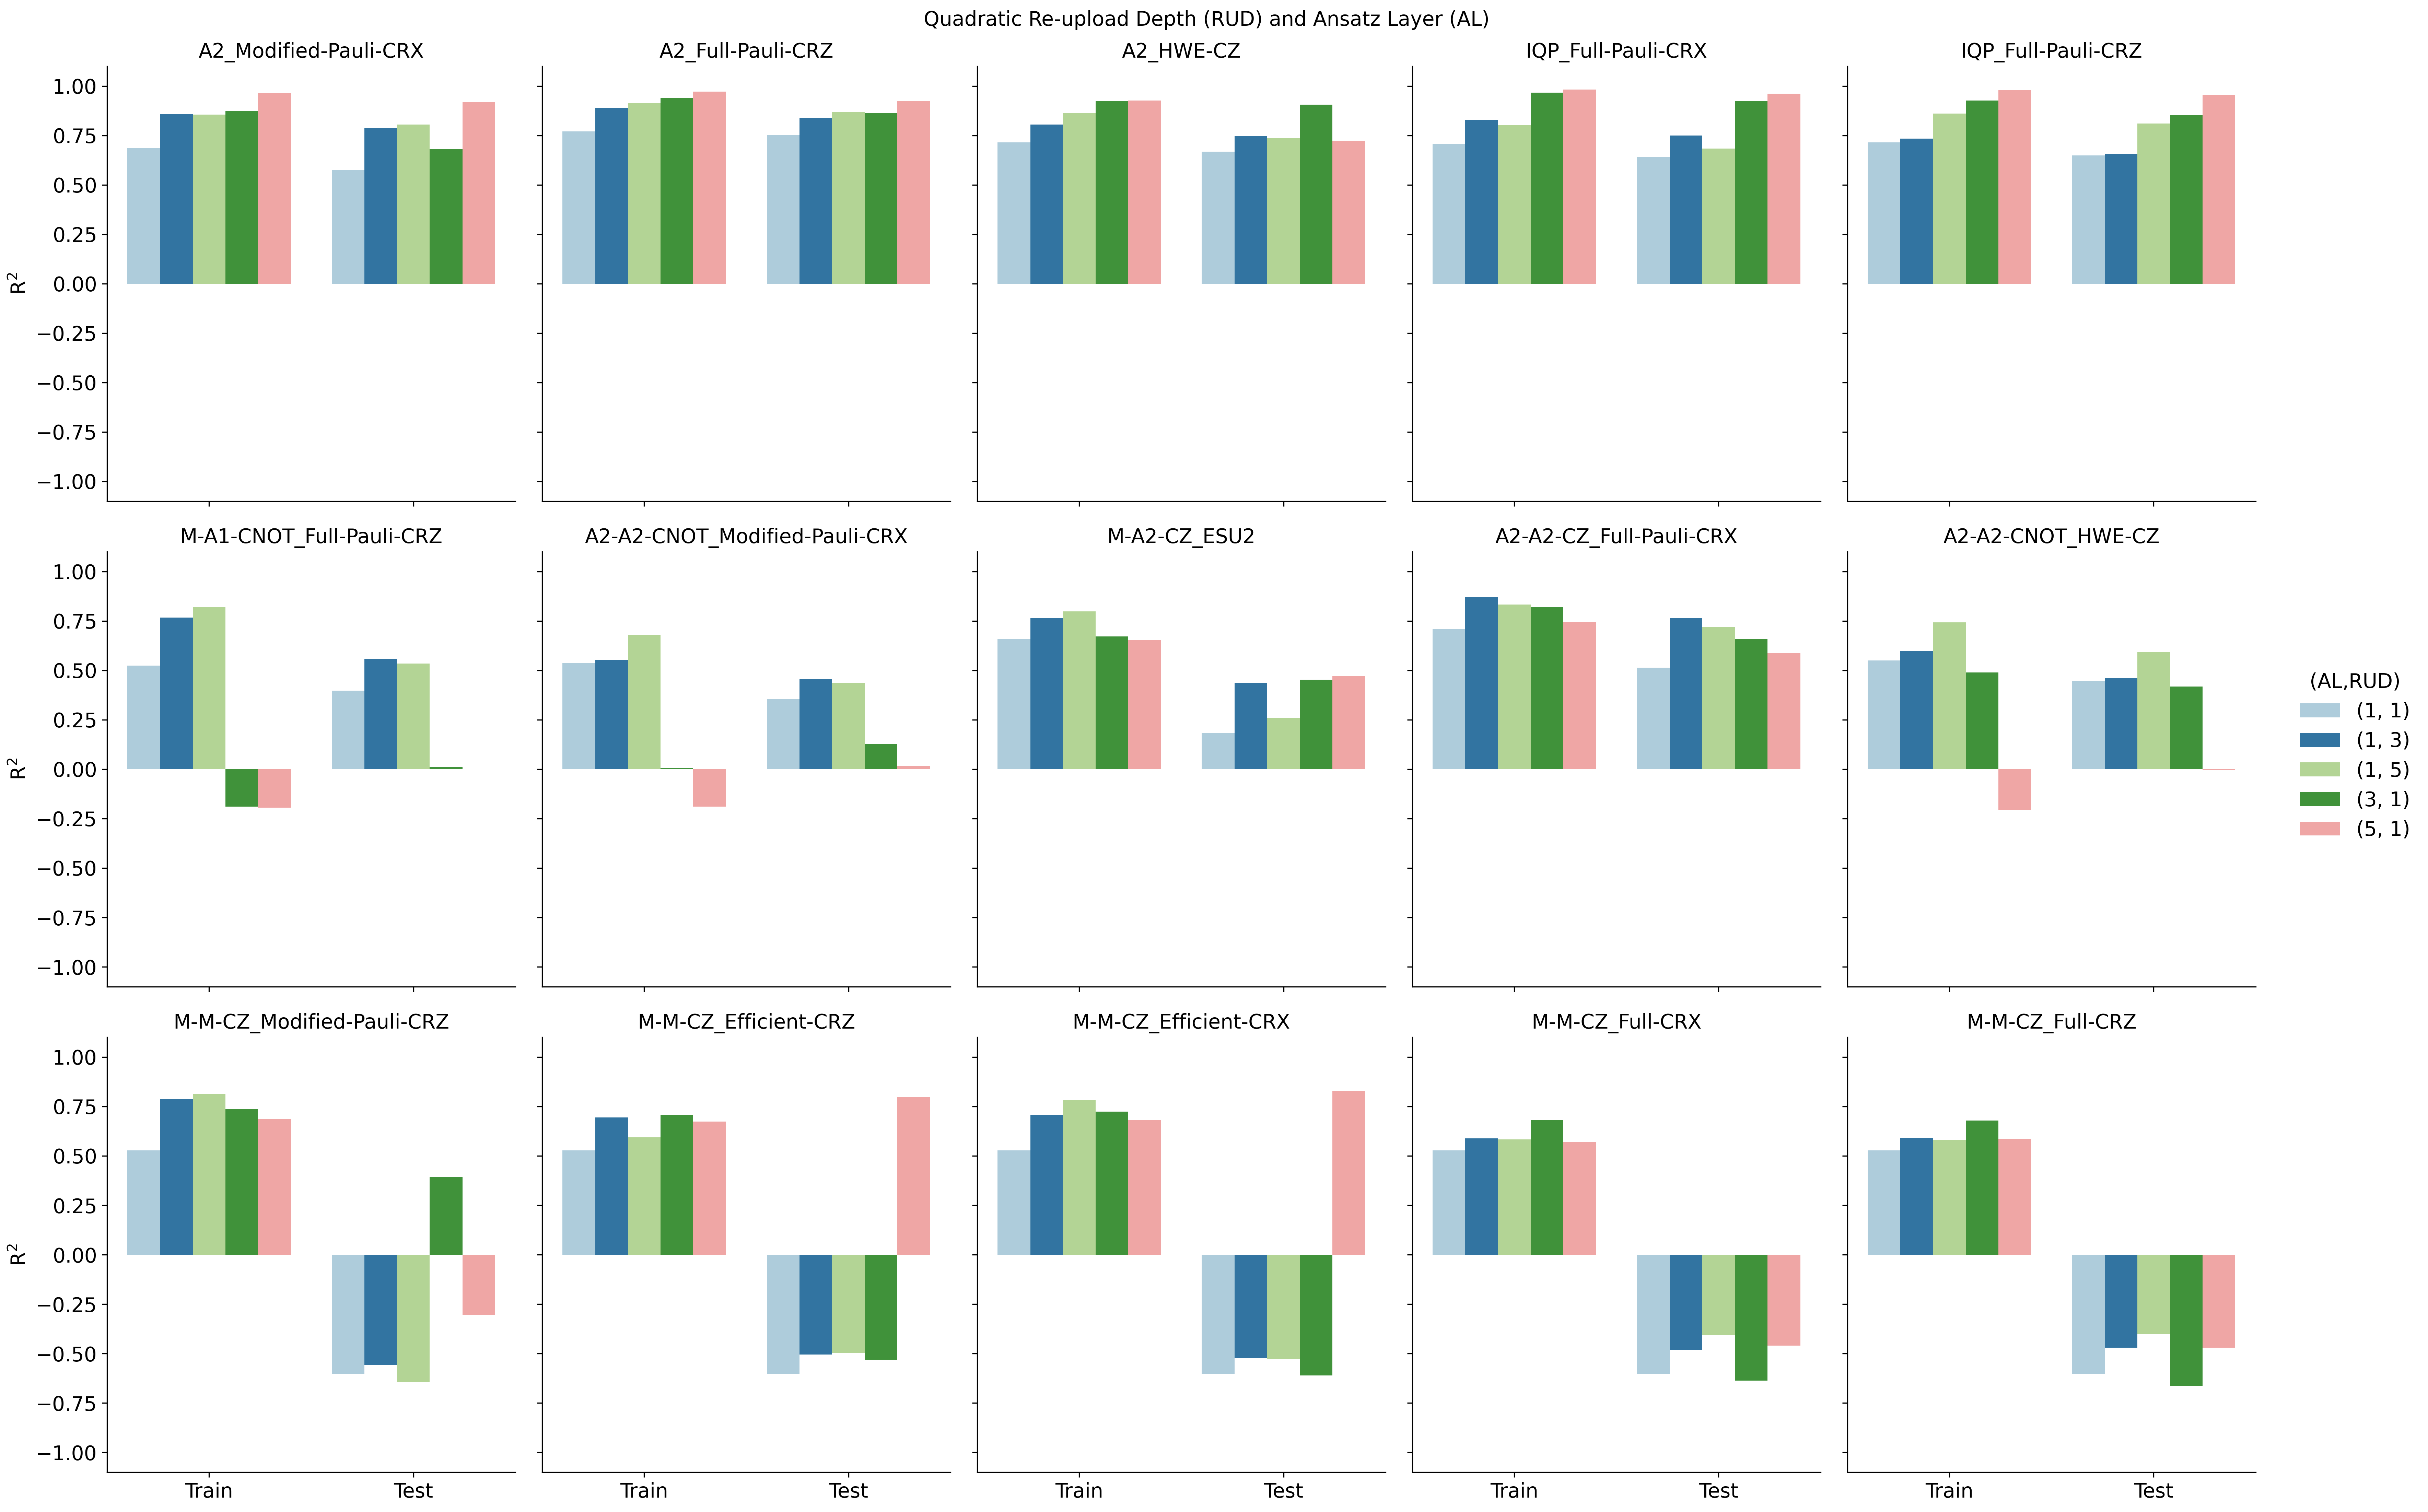
\includegraphics[width=\linewidth]{../images/Function_Fitting/sixteenqubit/16qubit_Quadratic_RUD_AL}
		\caption{}
		\label{fig:16qubit_Quadratic_RUD_AL}
	\end{subfigure}
	\hfill
%	\begin{subfigure}[b]{0.49\textwidth}
%		\centering
%		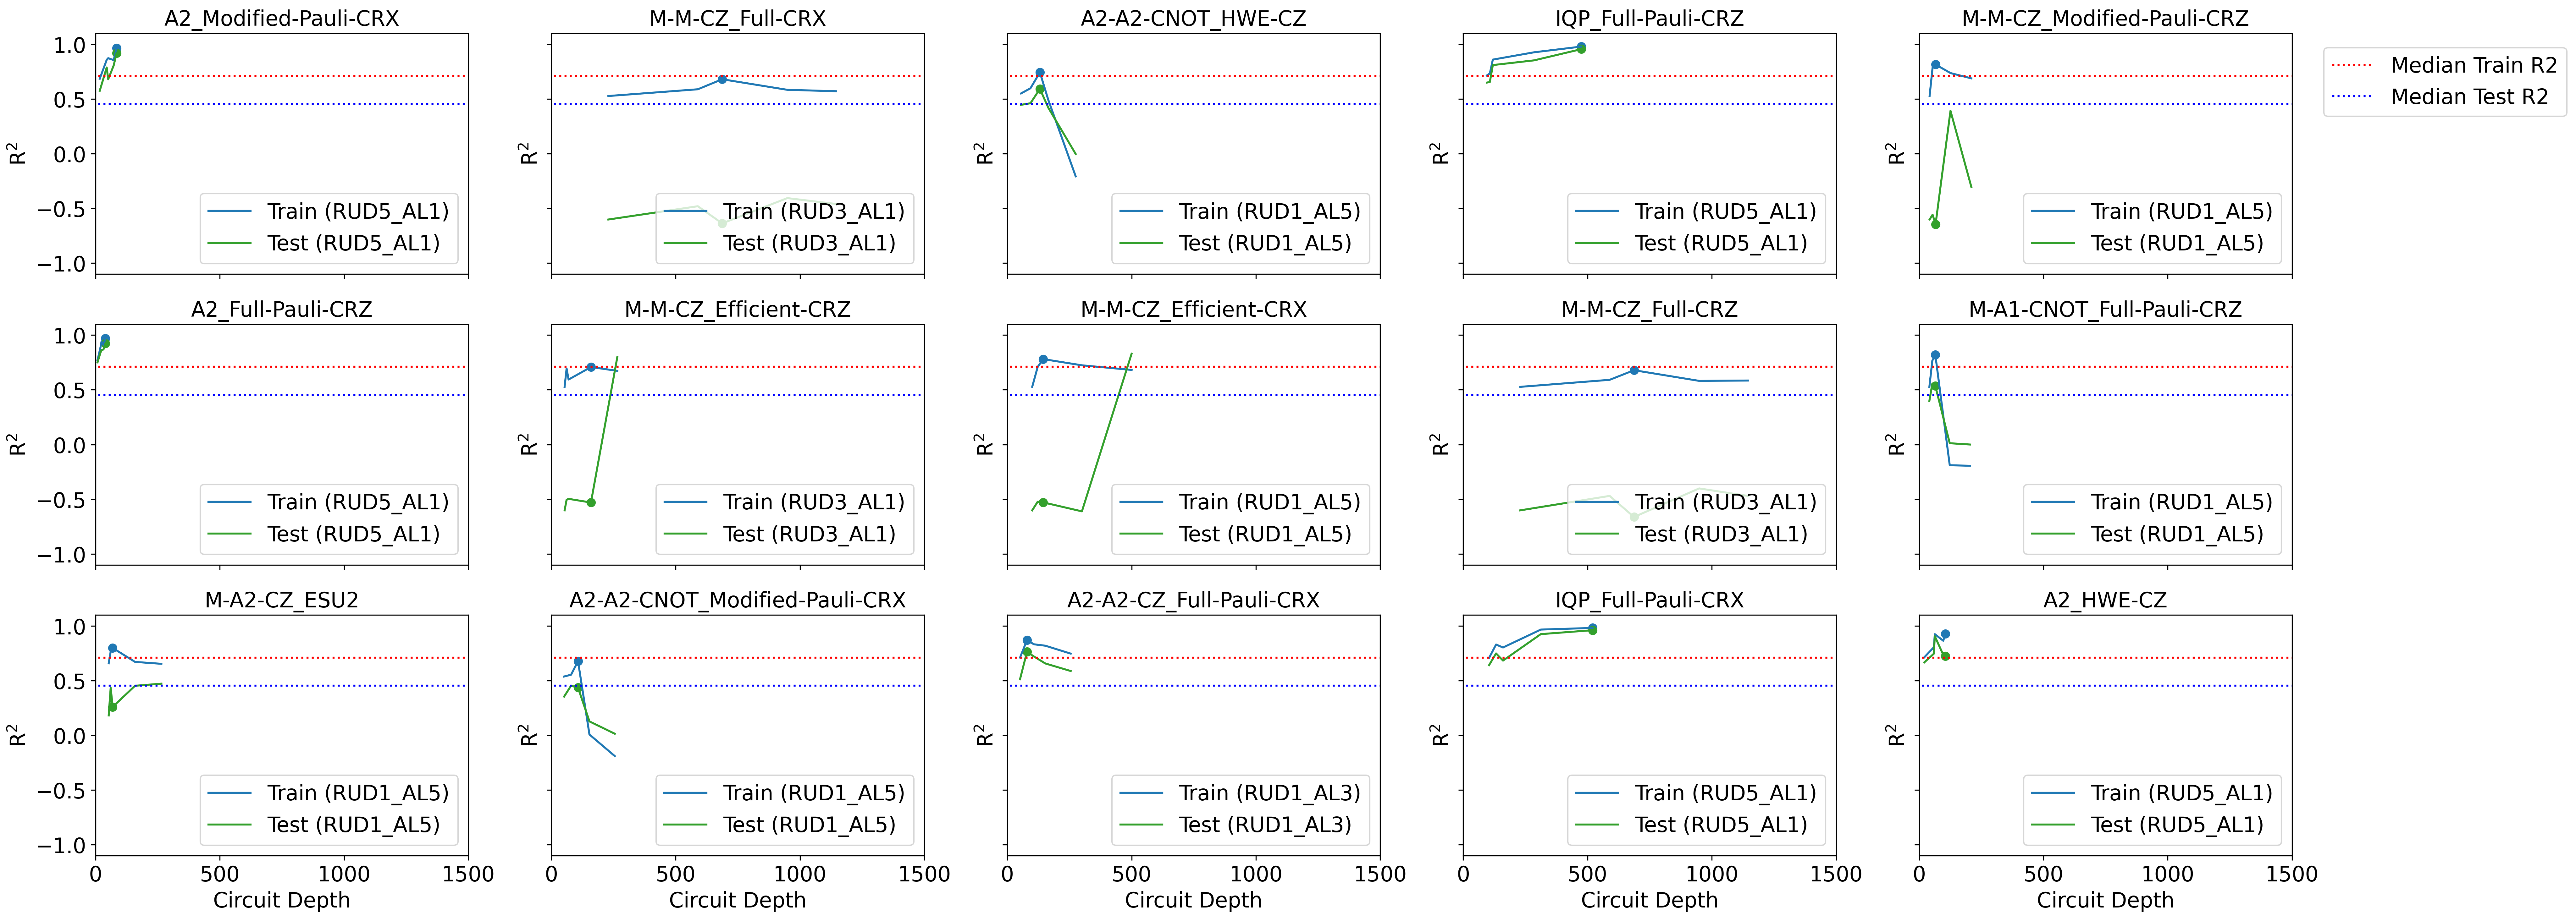
\includegraphics[width=\linewidth]{../images/Function_Fitting/quadratic_circuitdepth_vs_R2}
%		\caption{}
%		\label{fig:quadratic_circuitdepth_vs_R2}
%	\end{subfigure}
%	\hfill		
	\begin{subfigure}[b]{0.49\textwidth}
		\centering
		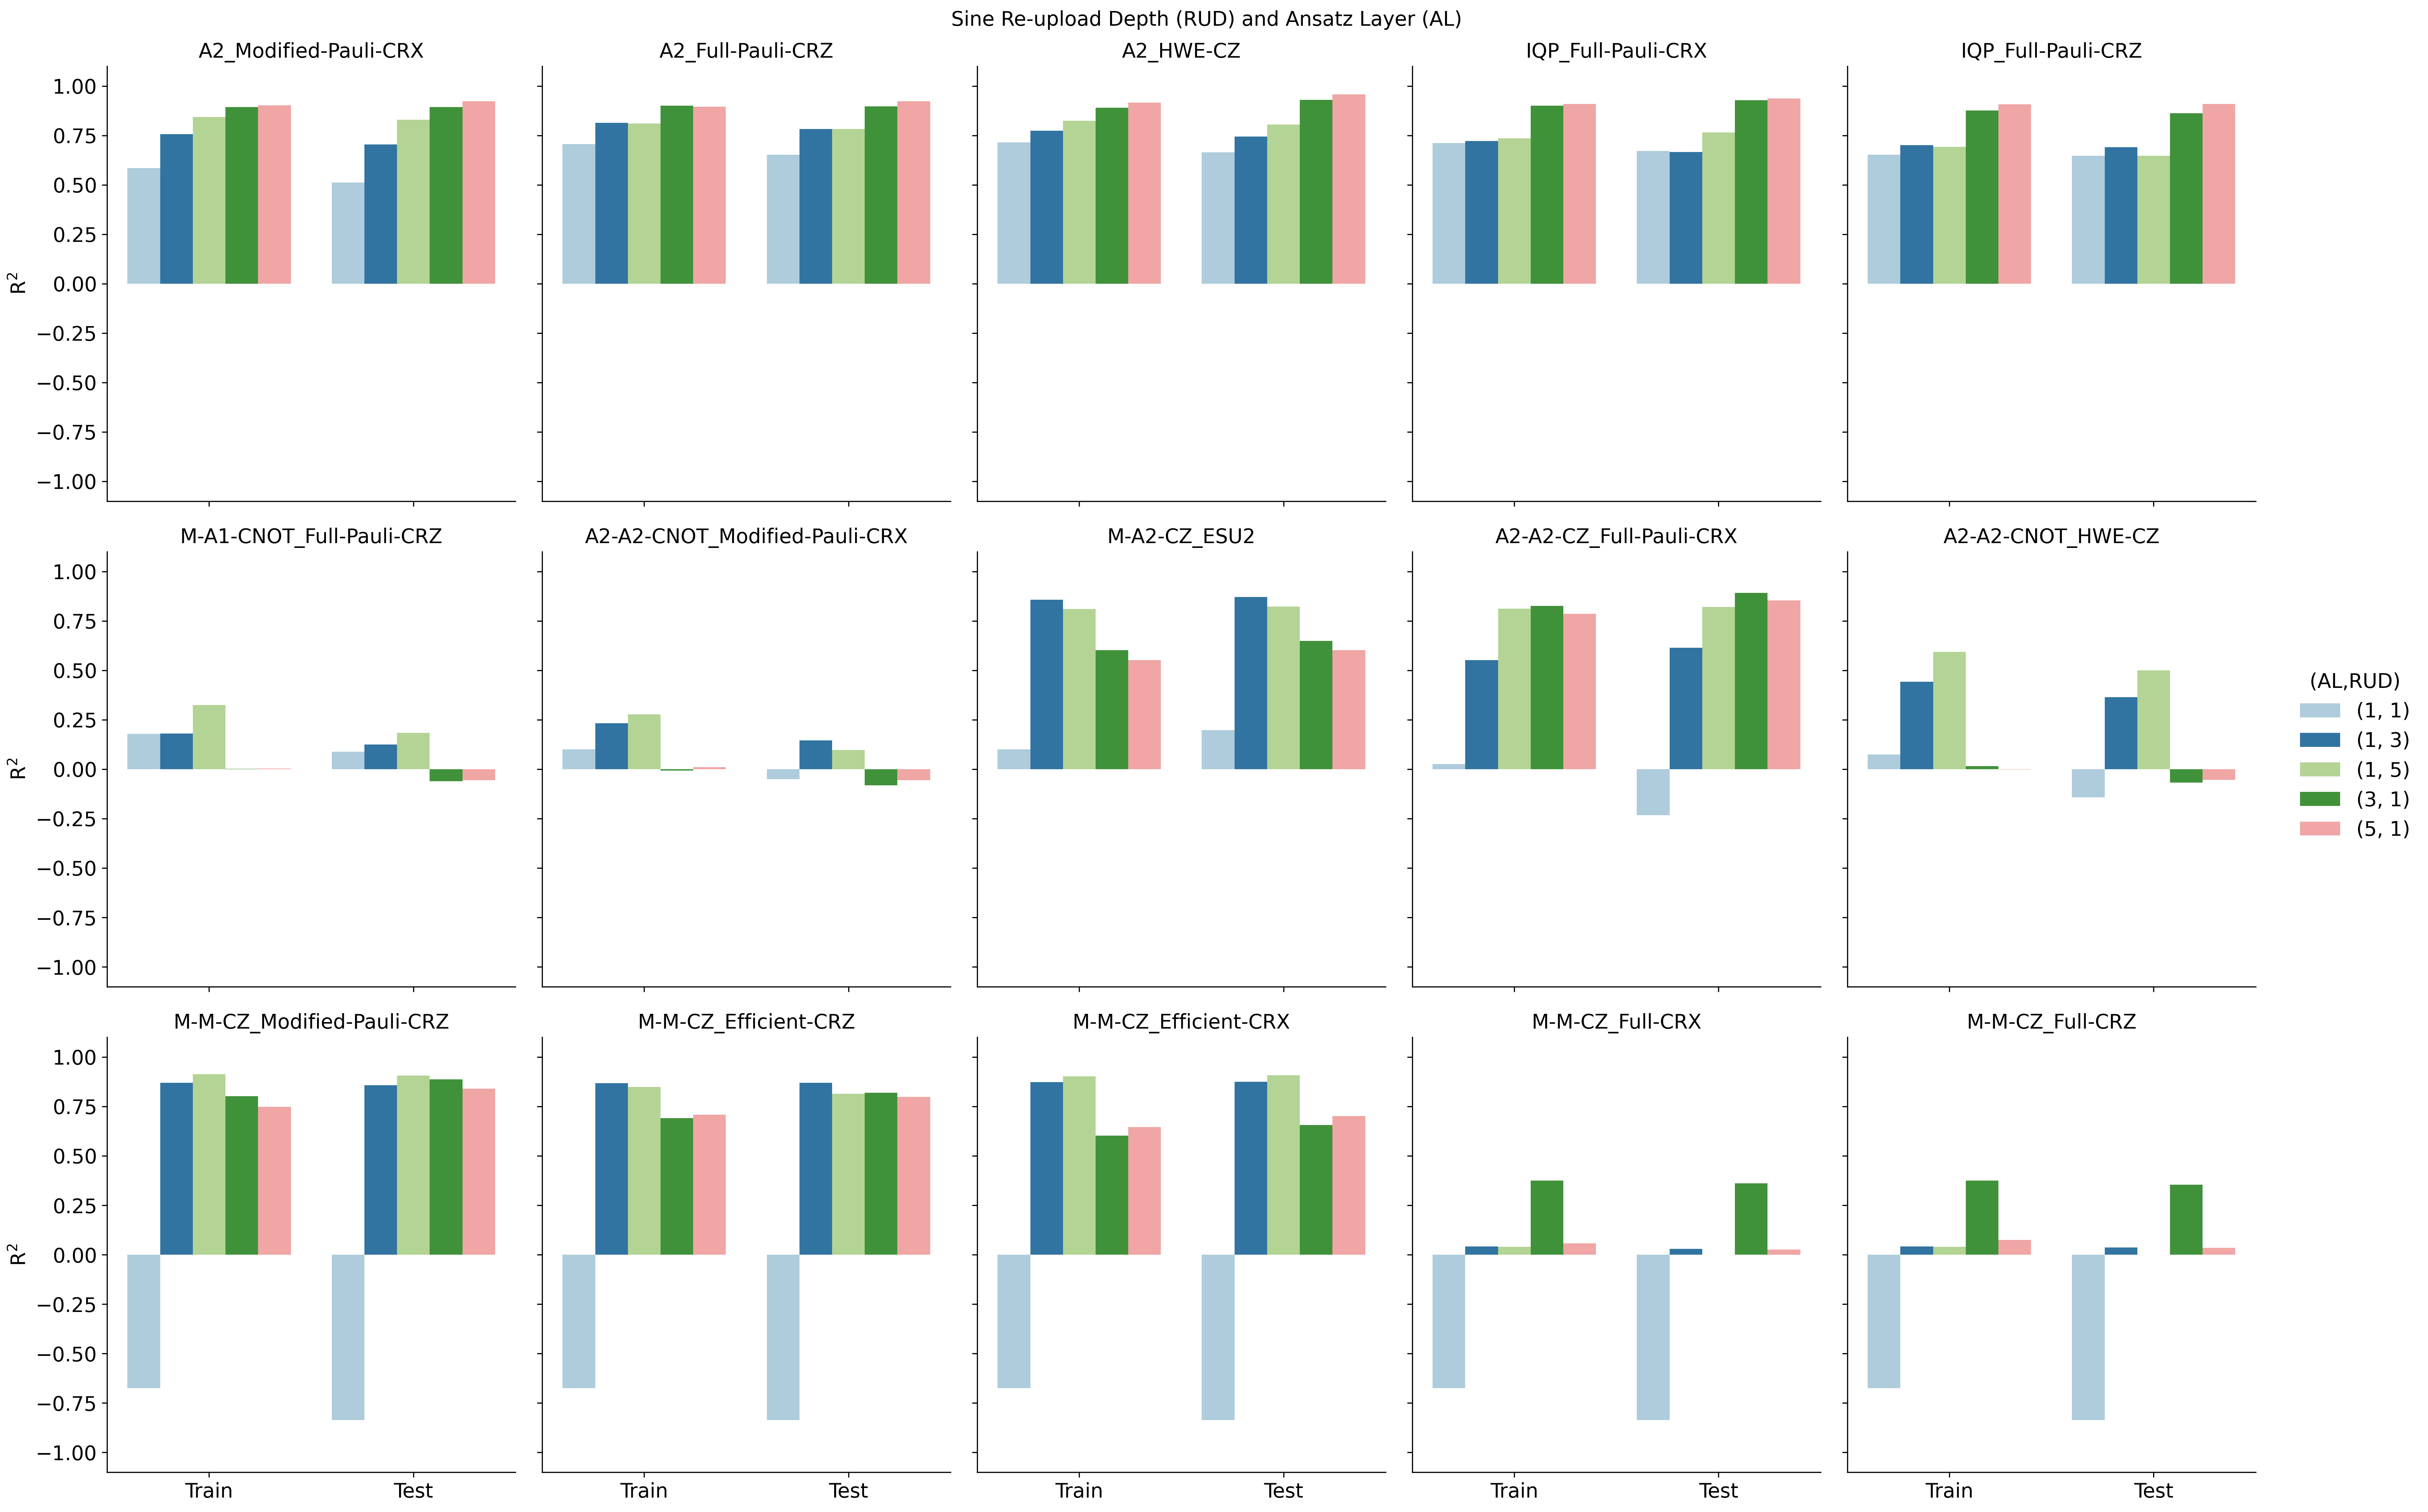
\includegraphics[width=\linewidth]{../images/Function_Fitting/sixteenqubit/16qubit_Sine_RUD_AL.png}
		\caption{}
		\label{fig:16qubit_Sine_RUD_AL}
	\end{subfigure}	
	\hfill
%	\begin{subfigure}[b]{0.49\textwidth}
%		\centering
%		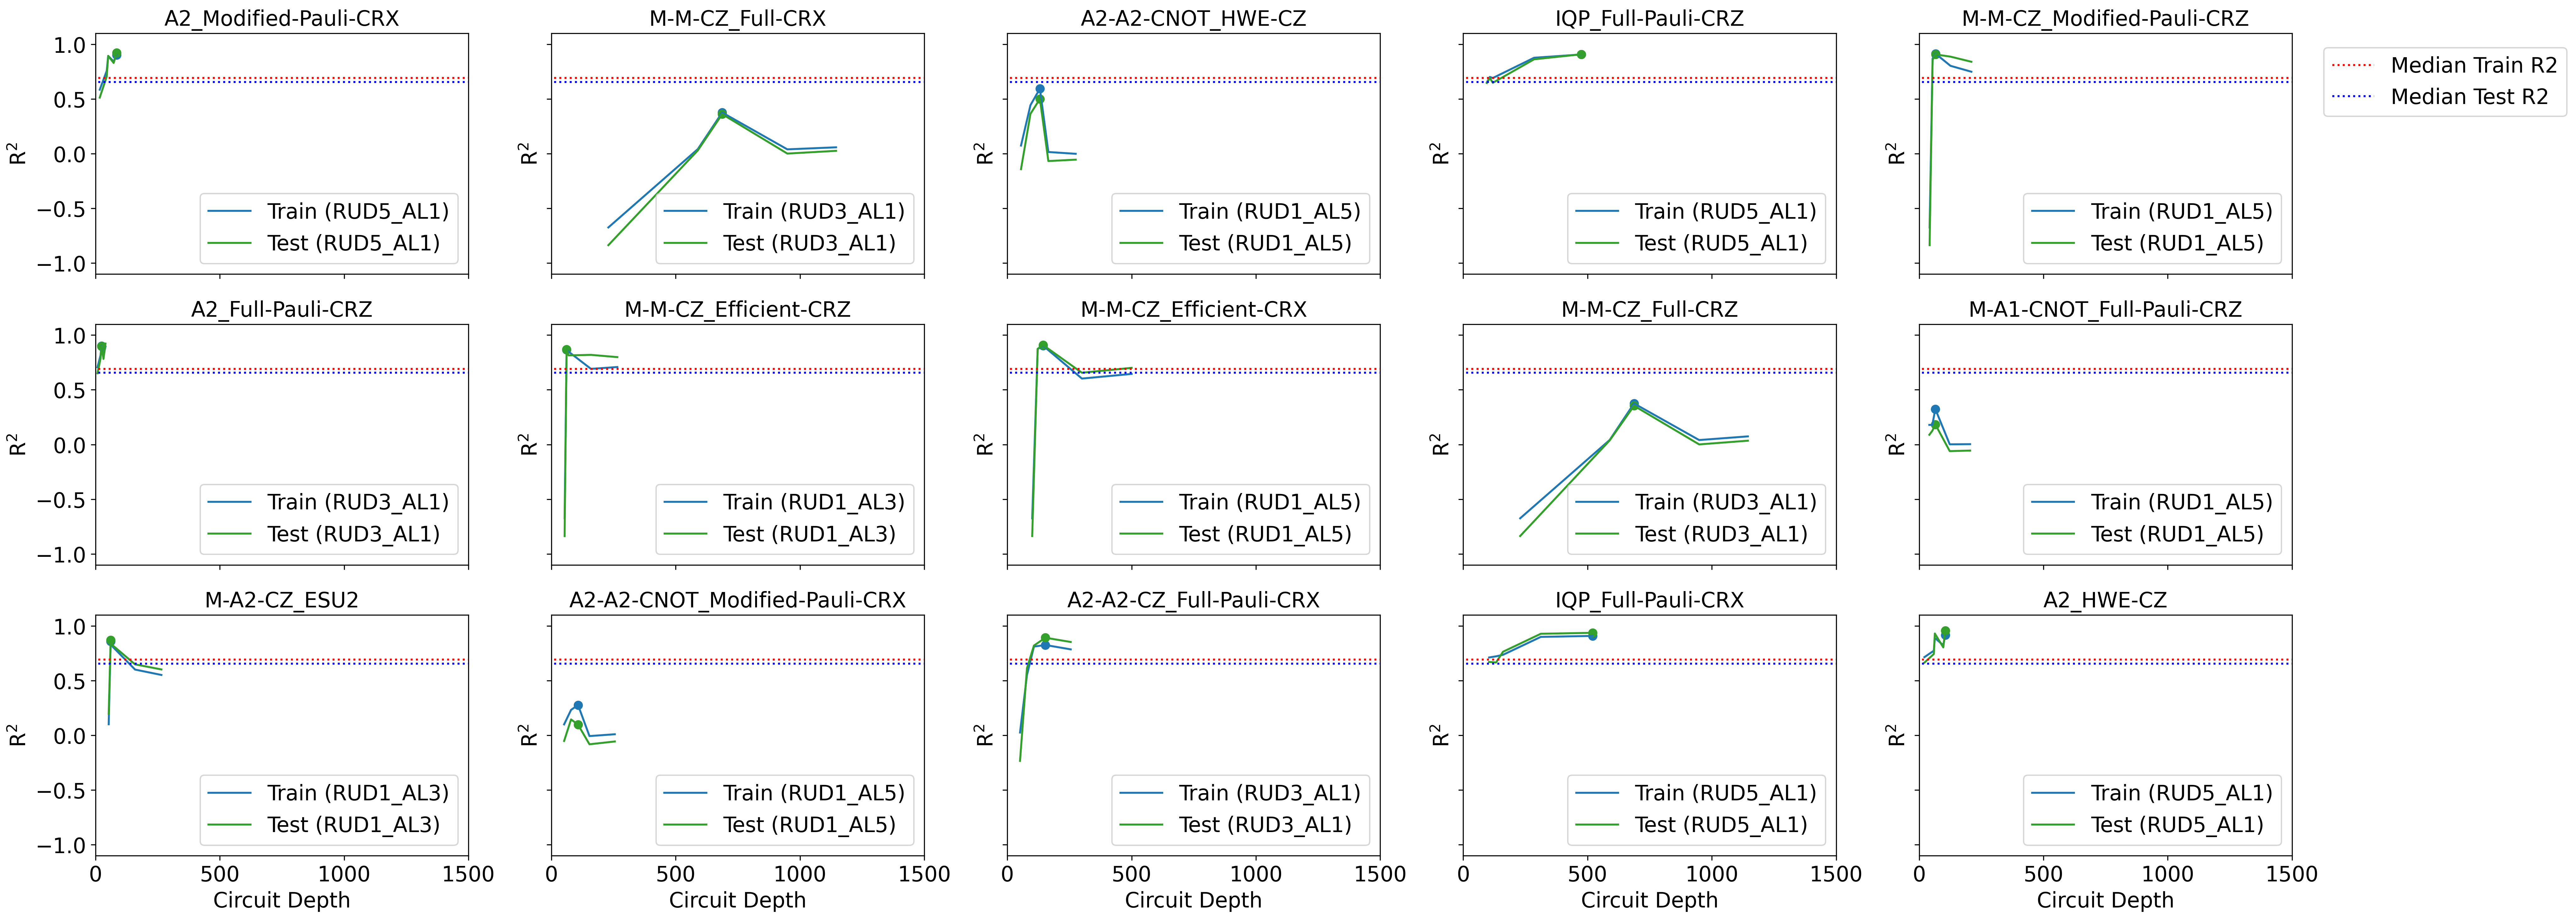
\includegraphics[width=\linewidth]{../images/Function_Fitting/sine_circuitdepth_vs_R2}
%		\caption{}
%		\label{fig:sine_circuitdepth_vs_R2}
%	\end{subfigure}
%	\hfill		
	\caption{The best five (top row), median five (middle row), and worst five (bottom row) circuits for the 16 qubit (a) linear, (b) quadratic, and (c) sine data show that, in general, an increase in the re-upload depth (RUD) or ansatz layers (AL) increases model performance (R$^{2}$ shown on the y-axis).}
	\label{fig:16qubit_RUD_AL}	
\end{figure}


One proposed advantage of using PQCs for ML tasks is that, in some cases, they can outperform classical ML models using less training data.\cite{hatakeyama-sato_quantum_2023}
We examine this phenomena with learning curves using the best performing circuits previously described.
The learning curves are generated by varying the percentage of training data from 10-80\% of the available data, while holding the number of test points to 10\% of the total data.
The three PQCs for each data set are compared to the classical models mentioned in subsection \ref{subsection:datasets} in a statistical manner (left sub-figures in Figs. \ref{fig:linear_learning_curves}, \ref{fig:quadratic_learning_curves}, and \ref{fig:sine_learning_curves}).
Across the full learning curve, IQP\_Full-Pauli-CRZ (linear function fitting) outperforms seven out of nine classical models for the training set and all of the classical models on the test set.
On the quadratic dataset, using IQP\_Full-Pauli-CRX, offers similar performance to the classical models, despite being outperformed on the training set across the learning curve. 
Similar to the IQP\_Full-Pauli-CRZ using the linear data, IQP\_Full-Pauli-CRX outperforms seven out of the nine classical models on the test set across the full learning curve.
On the sine data, A2\_HWE-CZ is consistent across the learning curve, outperforming six of the nine classical models on the training set and all of the models on the test set.
For all three datasets, this implies that the PQCs offer similar performance to classical models that do well on these datasets but provide better results on the test set.


\begin{figure}[H]
	\centering	
	\begin{subfigure}[b]{0.49\textwidth}
		\centering
		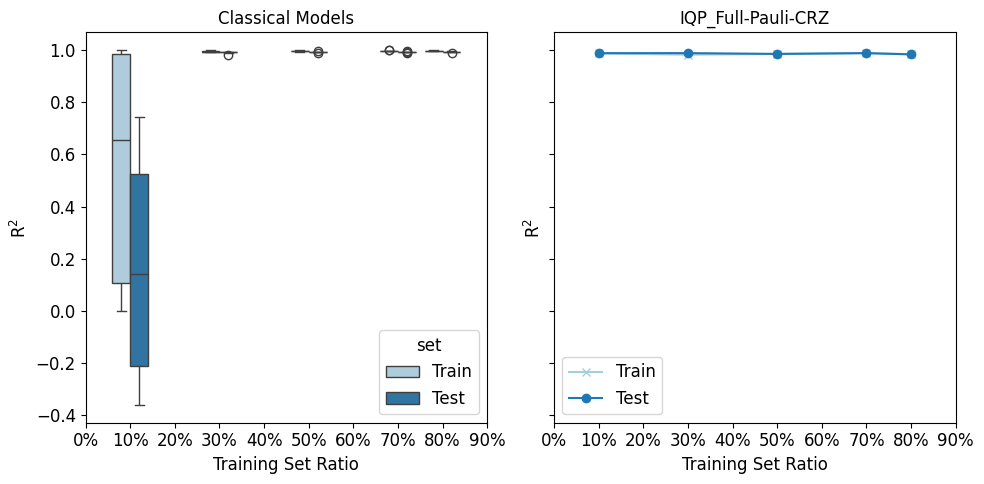
\includegraphics[width=\linewidth]{../images/Function_Fitting/linear_learning_curves.png}
		\caption{}
		\label{fig:linear_learning_curves}
	\end{subfigure}
	\hfill	
	\begin{subfigure}[b]{0.49\textwidth}
		\centering
		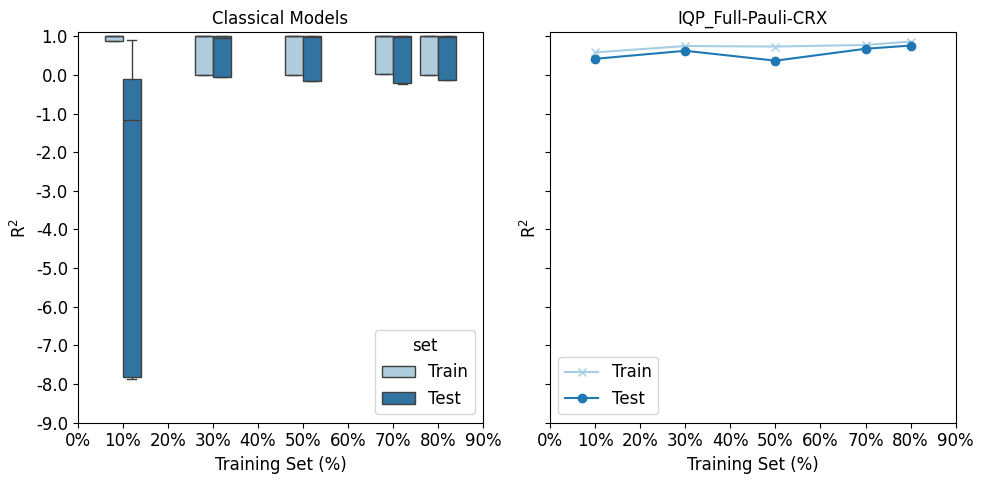
\includegraphics[width=\linewidth]{../images/Function_Fitting/quadratic_learning_curves.png}
		\caption{}
		\label{fig:quadratic_learning_curves}
	\end{subfigure}
	\hfill
	\begin{subfigure}[b]{0.49\textwidth}
		\centering
		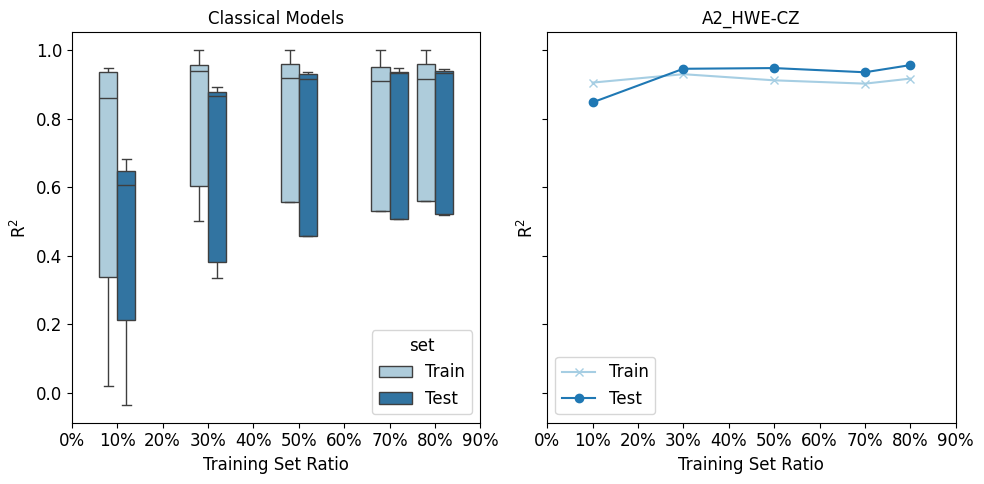
\includegraphics[width=\linewidth]{../images/Function_Fitting/sine_learning_curves.png}
		\caption{}
		\label{fig:sine_learning_curves}
	\end{subfigure}	
	\caption{Learning curves of the best PQCs (right side in the subfigures) versus various classical models (left side in the subfigure) for the (a) linear, (b) quadratic, and (c) sine function datasets.}
	\label{fig:functionfitting_learning_curves}	
\end{figure}


optimization level needs to be set to 0!

Lastly, using the function fitting datasets we analyze the effects of error mitigation on the model accuracy by comparing state vector simulations with noisy and error mitigated simulations using the \textit{fake\_quebec} backend.
Initially, we explored two different methods of error mitigation zero-noise extrapolation (ZNE) using MITIQ\cite{larose_mitiq_2022} and TREX, as implemented in Qiskit. 
We found that both linear and Richardson ZNE were too costly to simulate on classical computers using 16 qubits for all three function fitting datasets and chose only to use TREX for error mitigation.
Our analysis revealed that the state vector, TREX, and unmitigated IQP\_Full-Pauli-CRZ (linear function fitting data) models all have R$^{2}$ between 0.98 and 0.99, for both the training and test sets, as highlighted in Fig. \ref{fig:linear_error_mitigation}.
While the performance of the linear data can be attributed to the simiplicity of the dataset, for the quadratic function fitting data using IQP\_Full-Pauli-CRX (Fig. \ref{fig:quadratic_error_mitigation}), we found that the model with unmitigated error has an R$^{2}$ of 0.65 for the training set and 0.45 for the test set.
This model is improved slightly by the incorporation of error mitigation using TREX, where the training set R$^{2}$ is 0.69 and test set R$^{2}$ is 0.60.
Overall, the model using TREX offers results more comparable to the state vector simulations, which has a R$^{2}$s of 0.80 and 0.68 for the training and test set, respectively.
On the sine function fitting data, using A2\_HWE-CZ (Fig. \ref{fig:sine_error_mitigation}), for the state vector, TREX, and unmitigated models, the training sets have R$^{2}$s of 0.92, 0.87, and 0.87, respectively, while the test sets have R$^{2}$s of 0.96, 0.89, and 0.91, respectively.
Overall, while these results are for simple function fitting data, we concluded that TREX offers a computational efficient error mitigation method, with results similar to the state vector calculations.0


\begin{figure}[H]
	\centering	
	\begin{subfigure}[b]{0.49\textwidth}
		\centering
		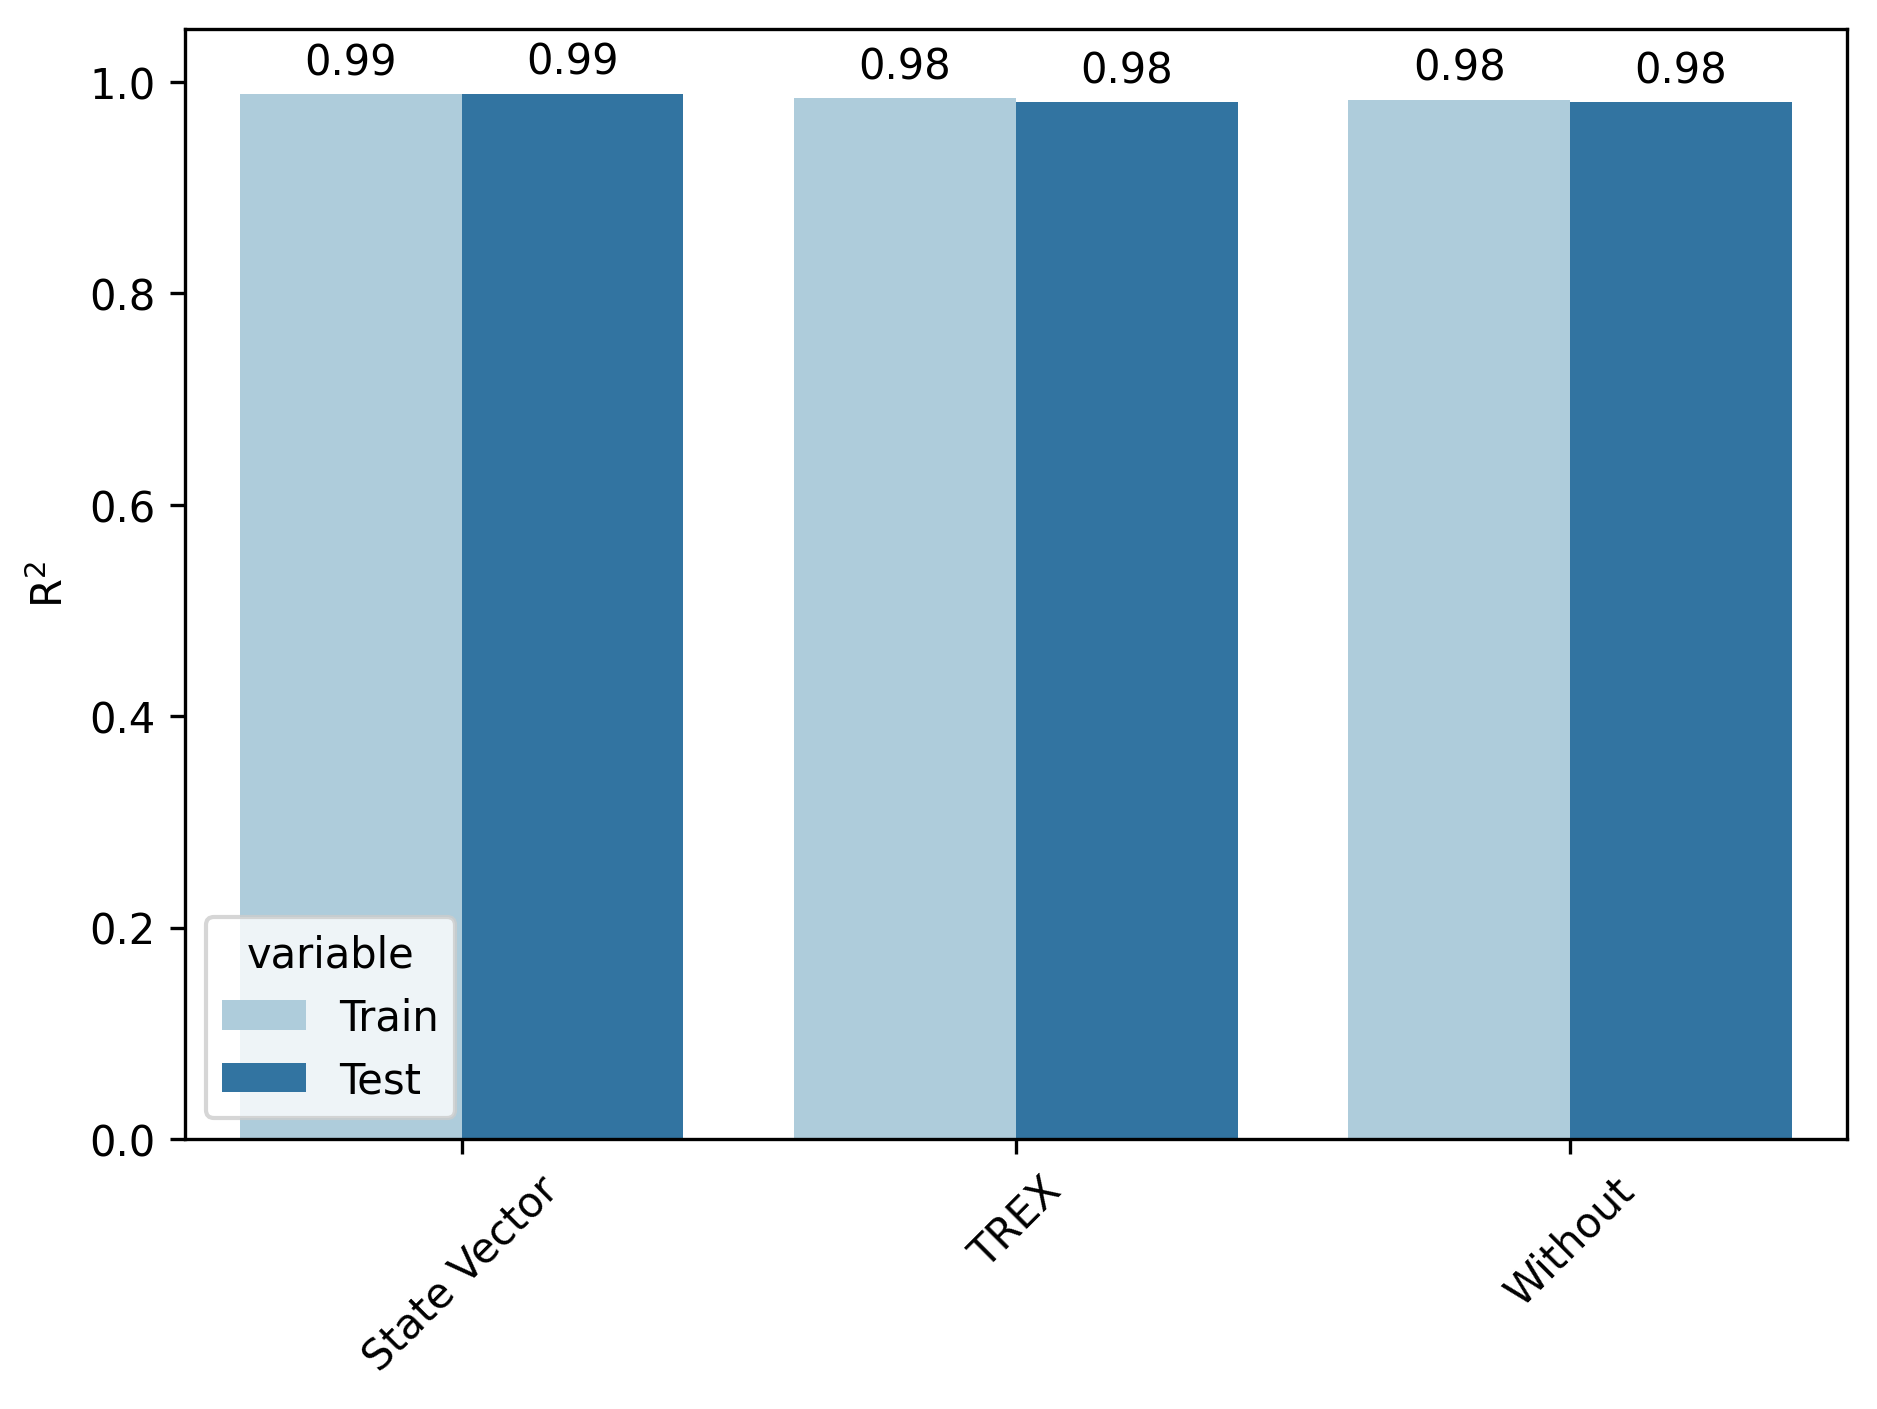
\includegraphics[width=\linewidth]{../images/Function_Fitting/linear_error_mitigation.png}
		\caption{}
		\label{fig:linear_error_mitigation}
	\end{subfigure}
	\hfill	
	\begin{subfigure}[b]{0.49\textwidth}
		\centering
		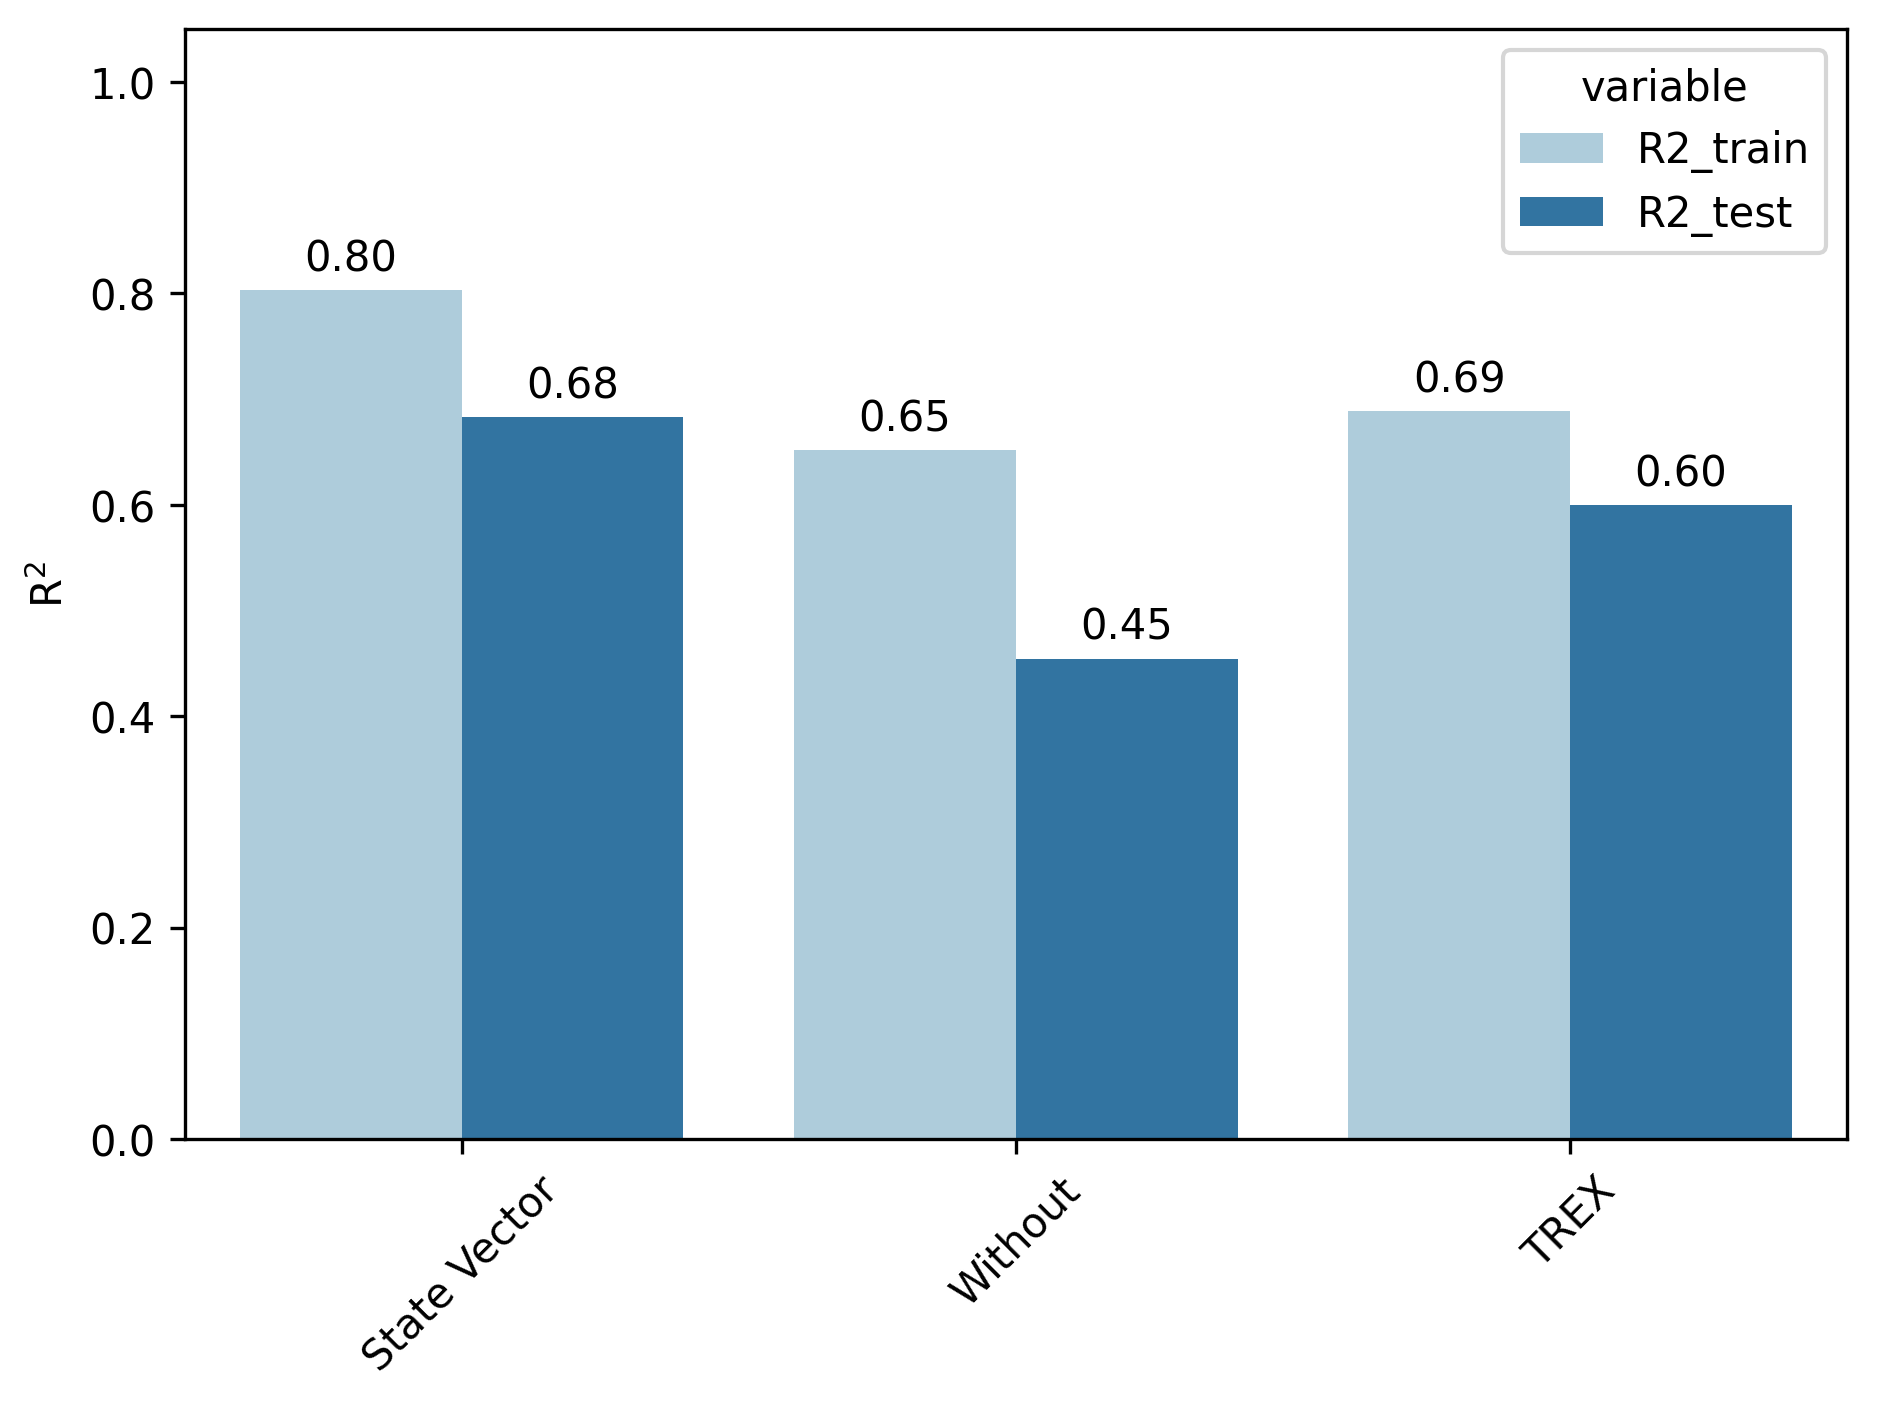
\includegraphics[width=\linewidth]{../images/Function_Fitting/quadratic_error_mitigation.png}
		\caption{}
		\label{fig:quadratic_error_mitigation}
	\end{subfigure}	
	\begin{subfigure}[b]{0.49\textwidth}
		\centering
		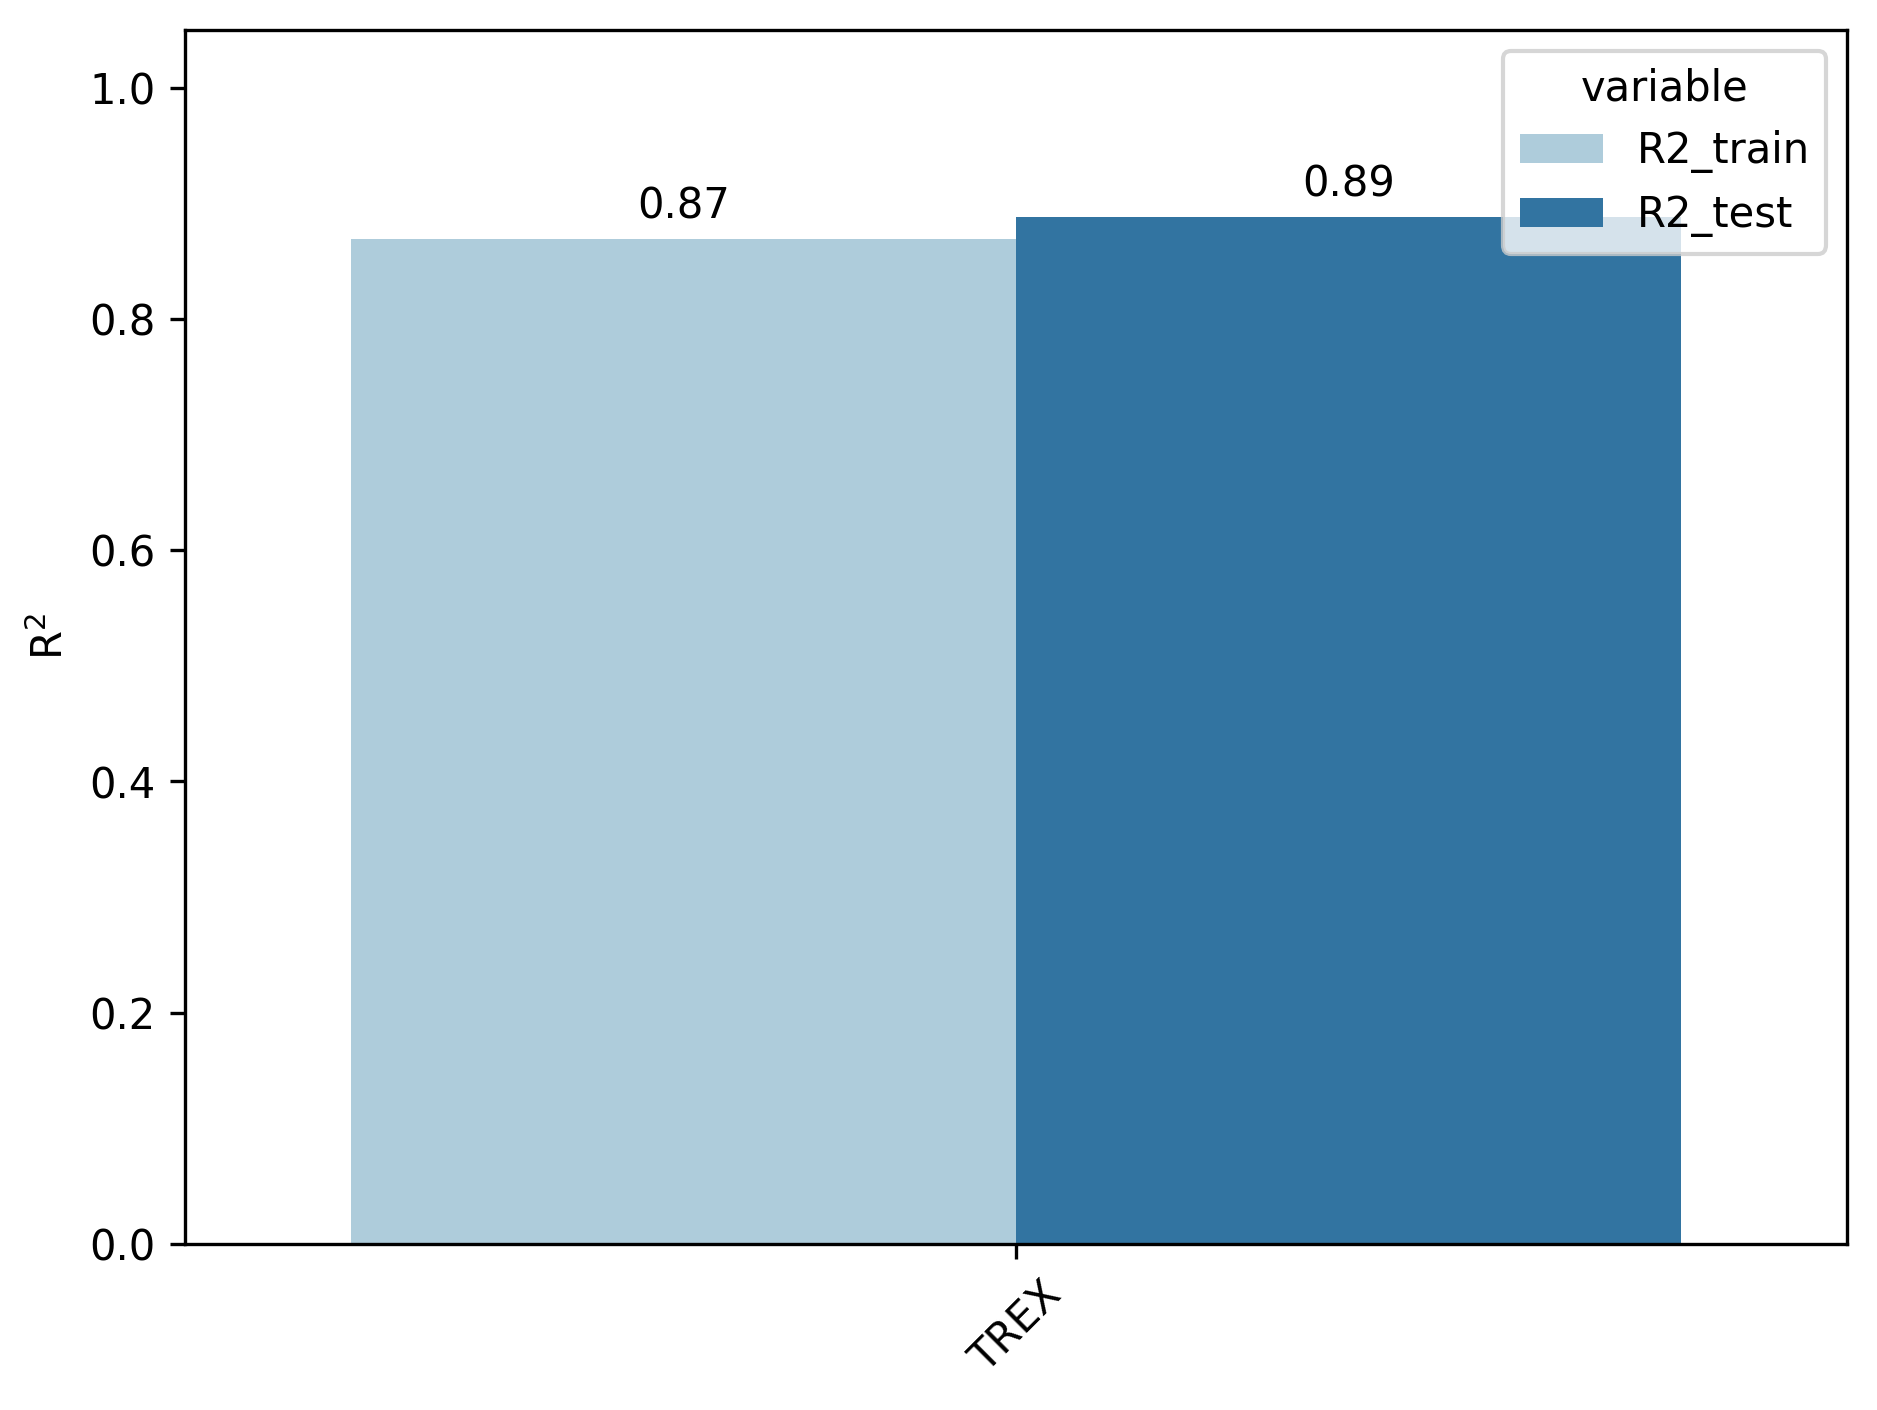
\includegraphics[width=\linewidth]{../images/Function_Fitting/sine_error_mitigation.png}
		\caption{}
		\label{fig:sine_error_mitigation}
	\end{subfigure}
	\hfill		
	\caption{Error mitigation benchmarking for the (a) linear, (b) quadratic, and (c) sine function comparing unmitigated and mitigated error using TREX with state vector simulations.}
	\label{fig:functionfitting_errormitigation}	
\end{figure}




\subsection{BSE}
The first chemically relevant dataset we explore is the BSE49 dataset.
As highlighted in Figs. \ref{fig:bondtypes} and \ref{fig:BSEdistr}, this dataset consists of a diverse set of representative chemical bonds and bond separation energies.
Herein, we follow a similar analysis to the function fitting data, starting off with an analysis of a large set of PQCs using five and sixteen qubits with RUDs and ALs of 1.
From these two sets of data, we choose the best two models to study how an increase in the RUD and AL effects model performance.
[learning curves]
[Conclude we do not want to run this on real hardware due to the lack of promising results using simulation]



five qubit \ref{fig:5BSE_heatplots} \ref{fig:5BSE_boxplots}
best encoder-ansatz pair: train R$^{2}$/test R$^{2}$
Best encoder on average train R$^{2}$/test R$^{2}$
Best ansatz on average train R$^{2}$/test R$^{2}$

'M-M-CNOT', '-0.0216'
'Full-CRX', '0.1214'

sixteen qubit \ref{fig:16BSE_heatplots} \ref{fig:16BSE_boxplots}
removed the really bad ones from five qubit
best encoder-ansatz pair: train R$^{2}$/test R$^{2}$
Best encoder on average train R$^{2}$/test R$^{2}$
Best ansatz on average train R$^{2}$/test R$^{2}$


\begin{figure}[H]
	\centering	
	\begin{subfigure}[b]{0.49\textwidth}
		\centering
		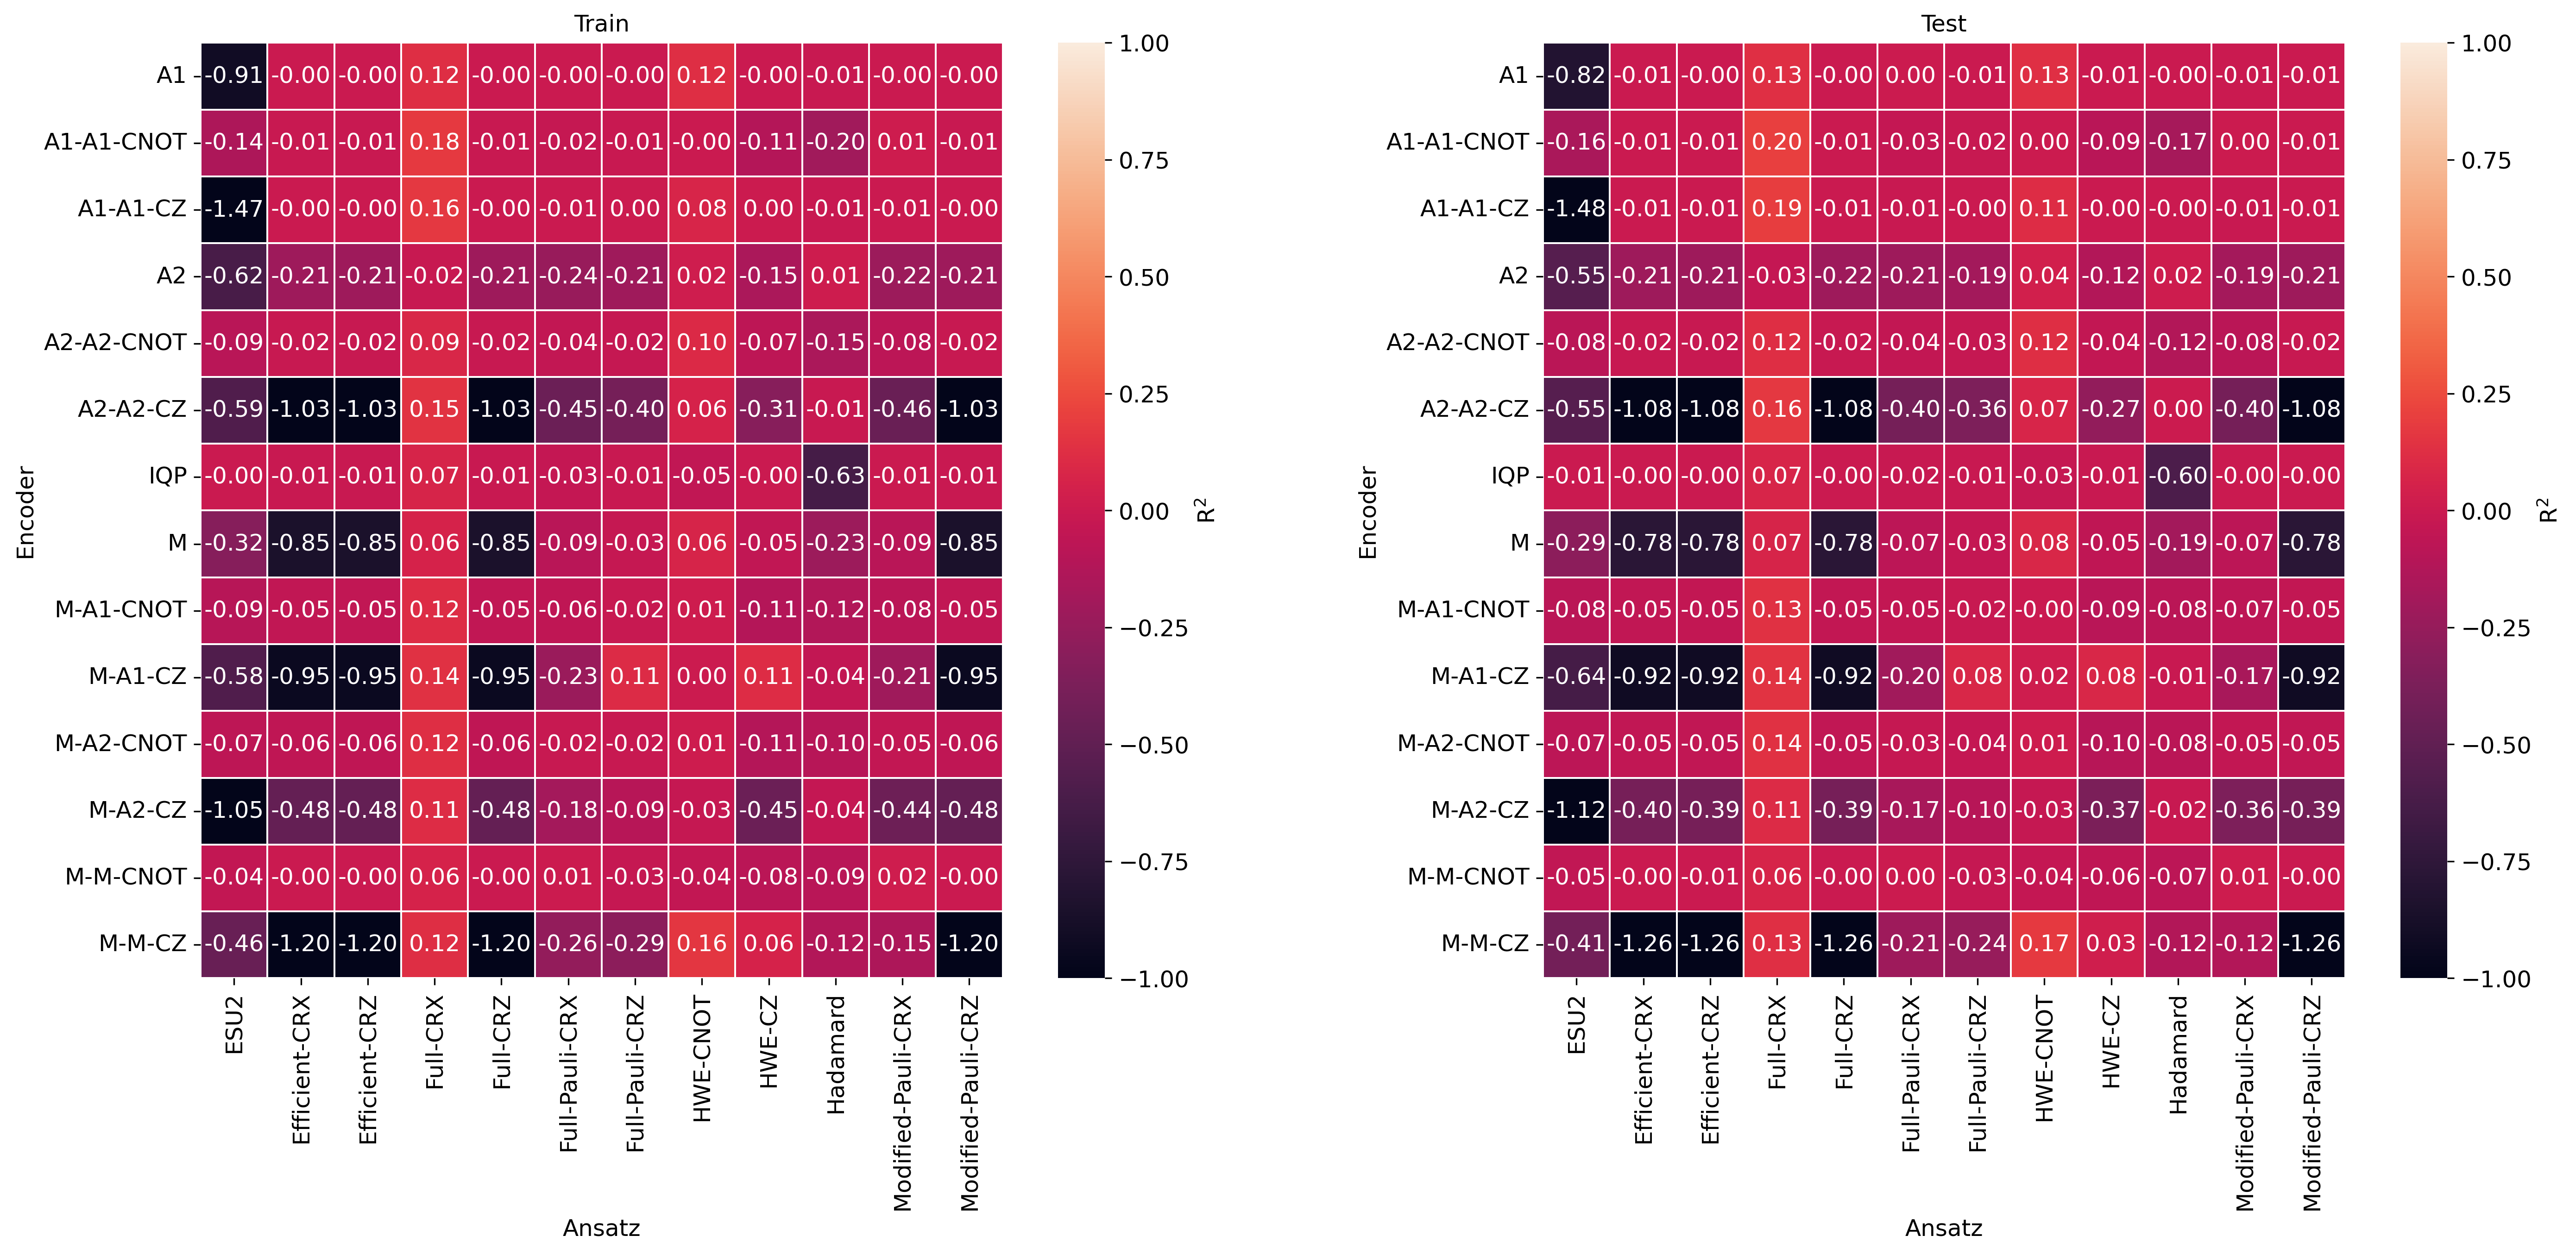
\includegraphics[width=\linewidth]{../images/BSE/fivequbit/BSE_heatplots}
		\caption{}
		\label{fig:5BSE_heatplots}
	\end{subfigure}
	\hfill
	\begin{subfigure}[b]{0.49\textwidth}
		\centering
		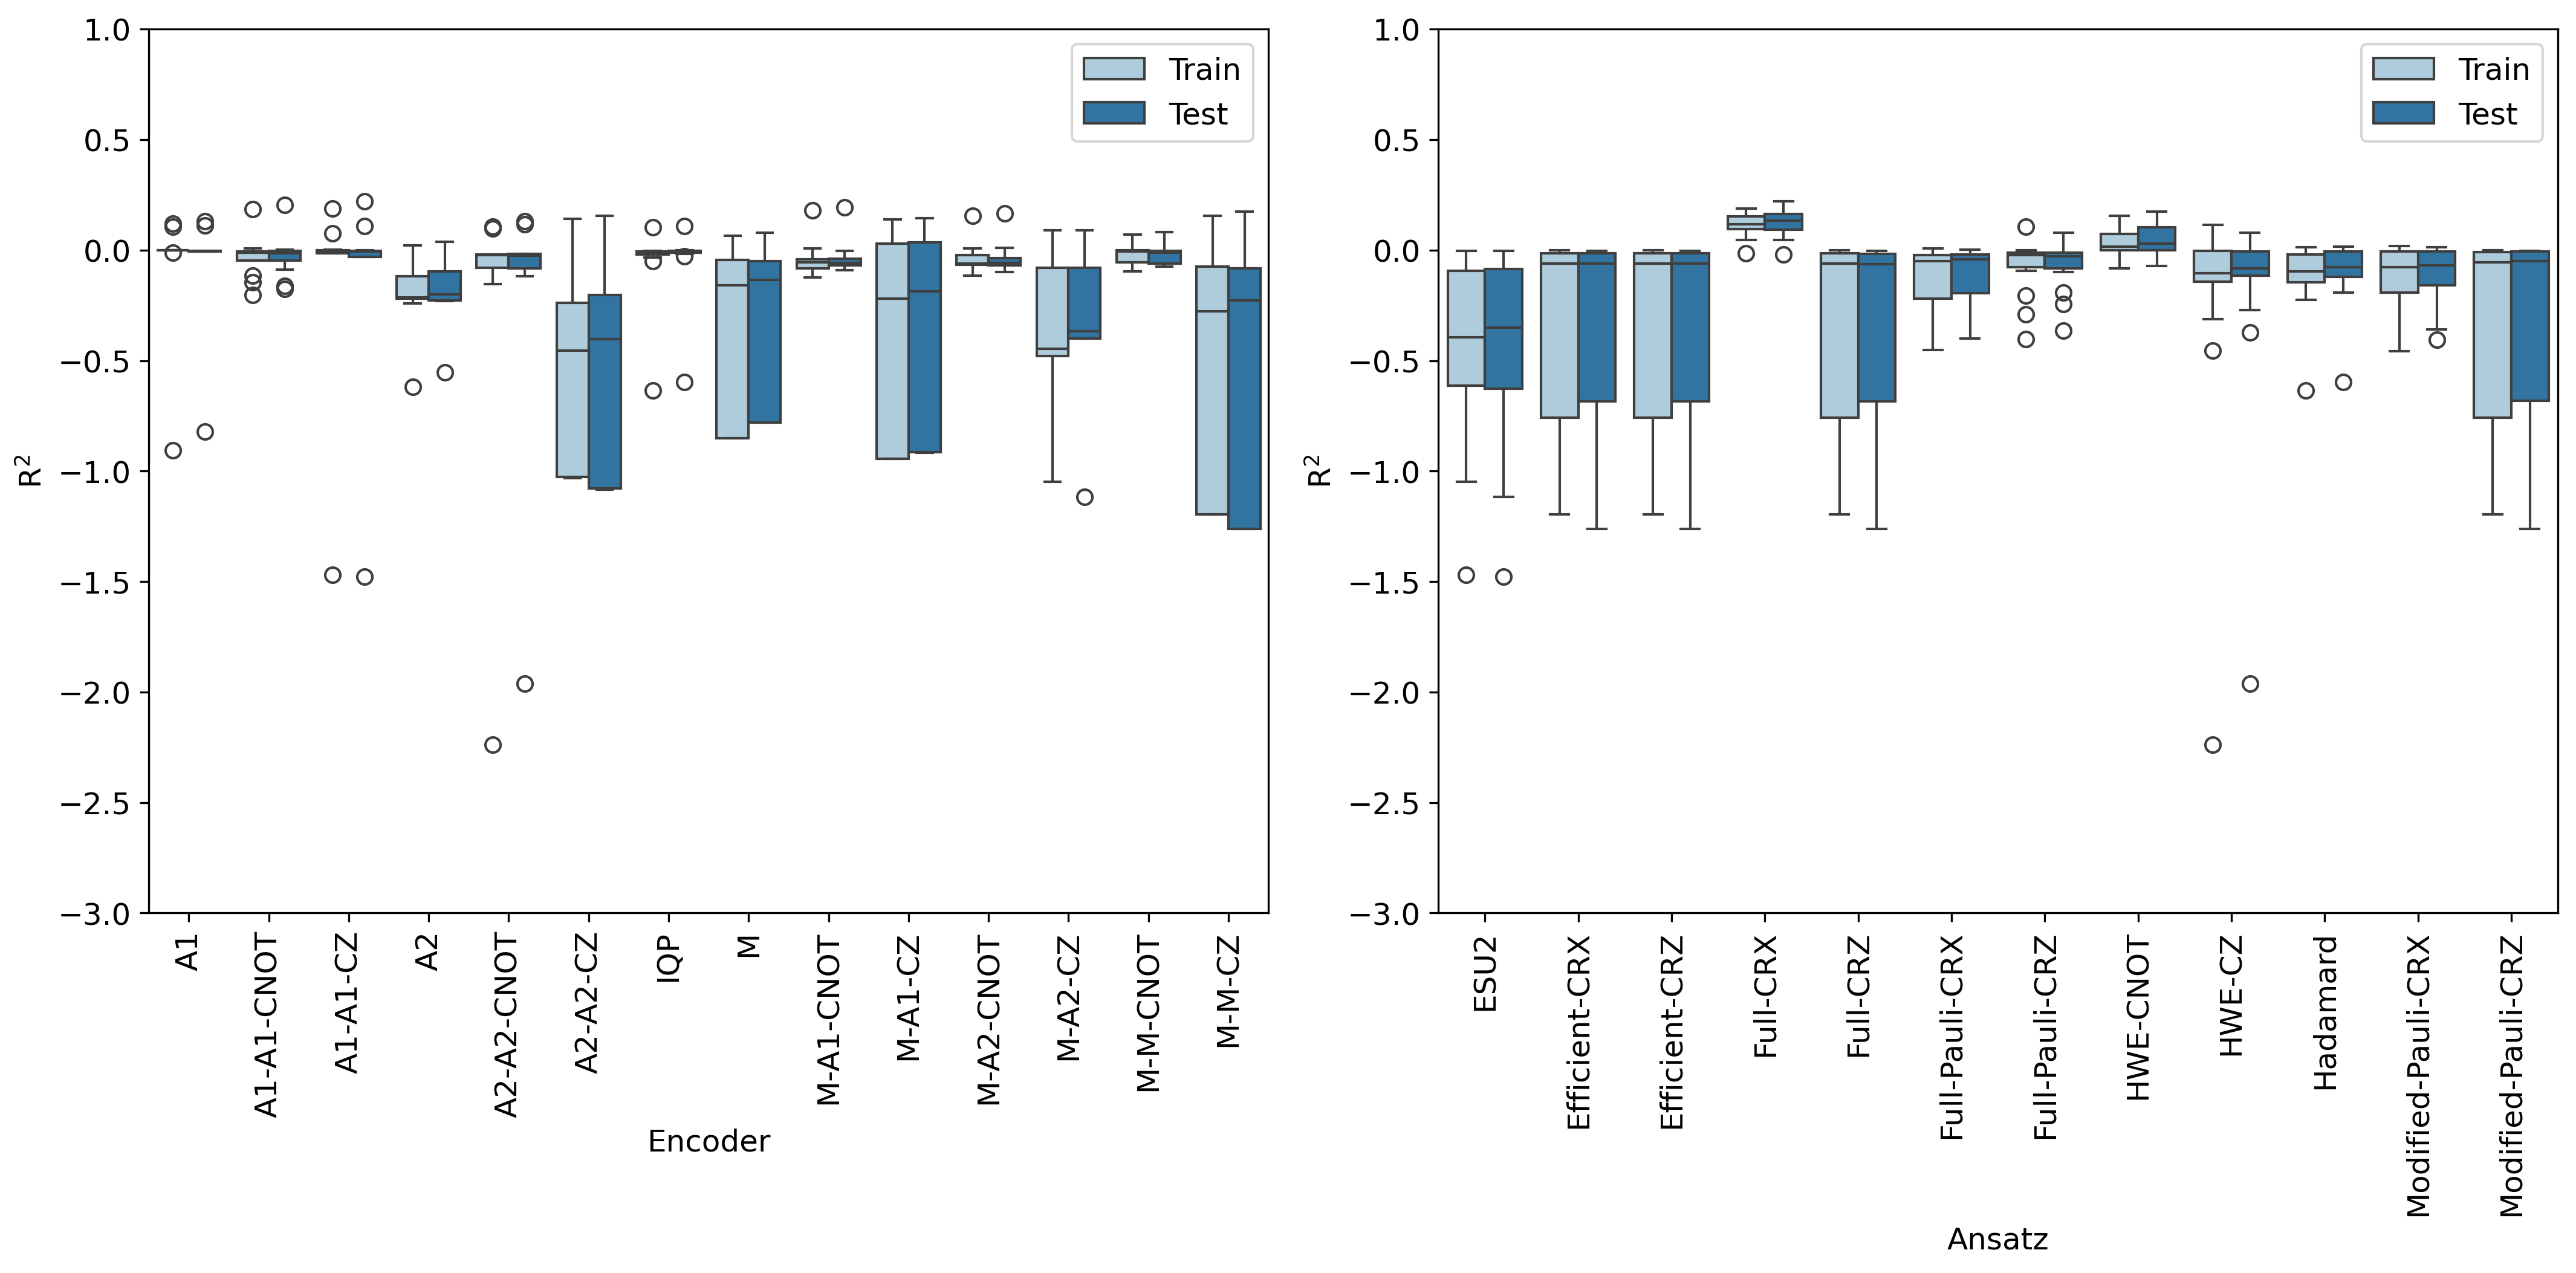
\includegraphics[width=\linewidth]{../images/BSE/fivequbit/BSE_boxplots}
		\caption{}
		\label{fig:5BSE_boxplots}
	\end{subfigure}
	\hfill
	\begin{subfigure}[b]{0.49\textwidth}
		\centering
		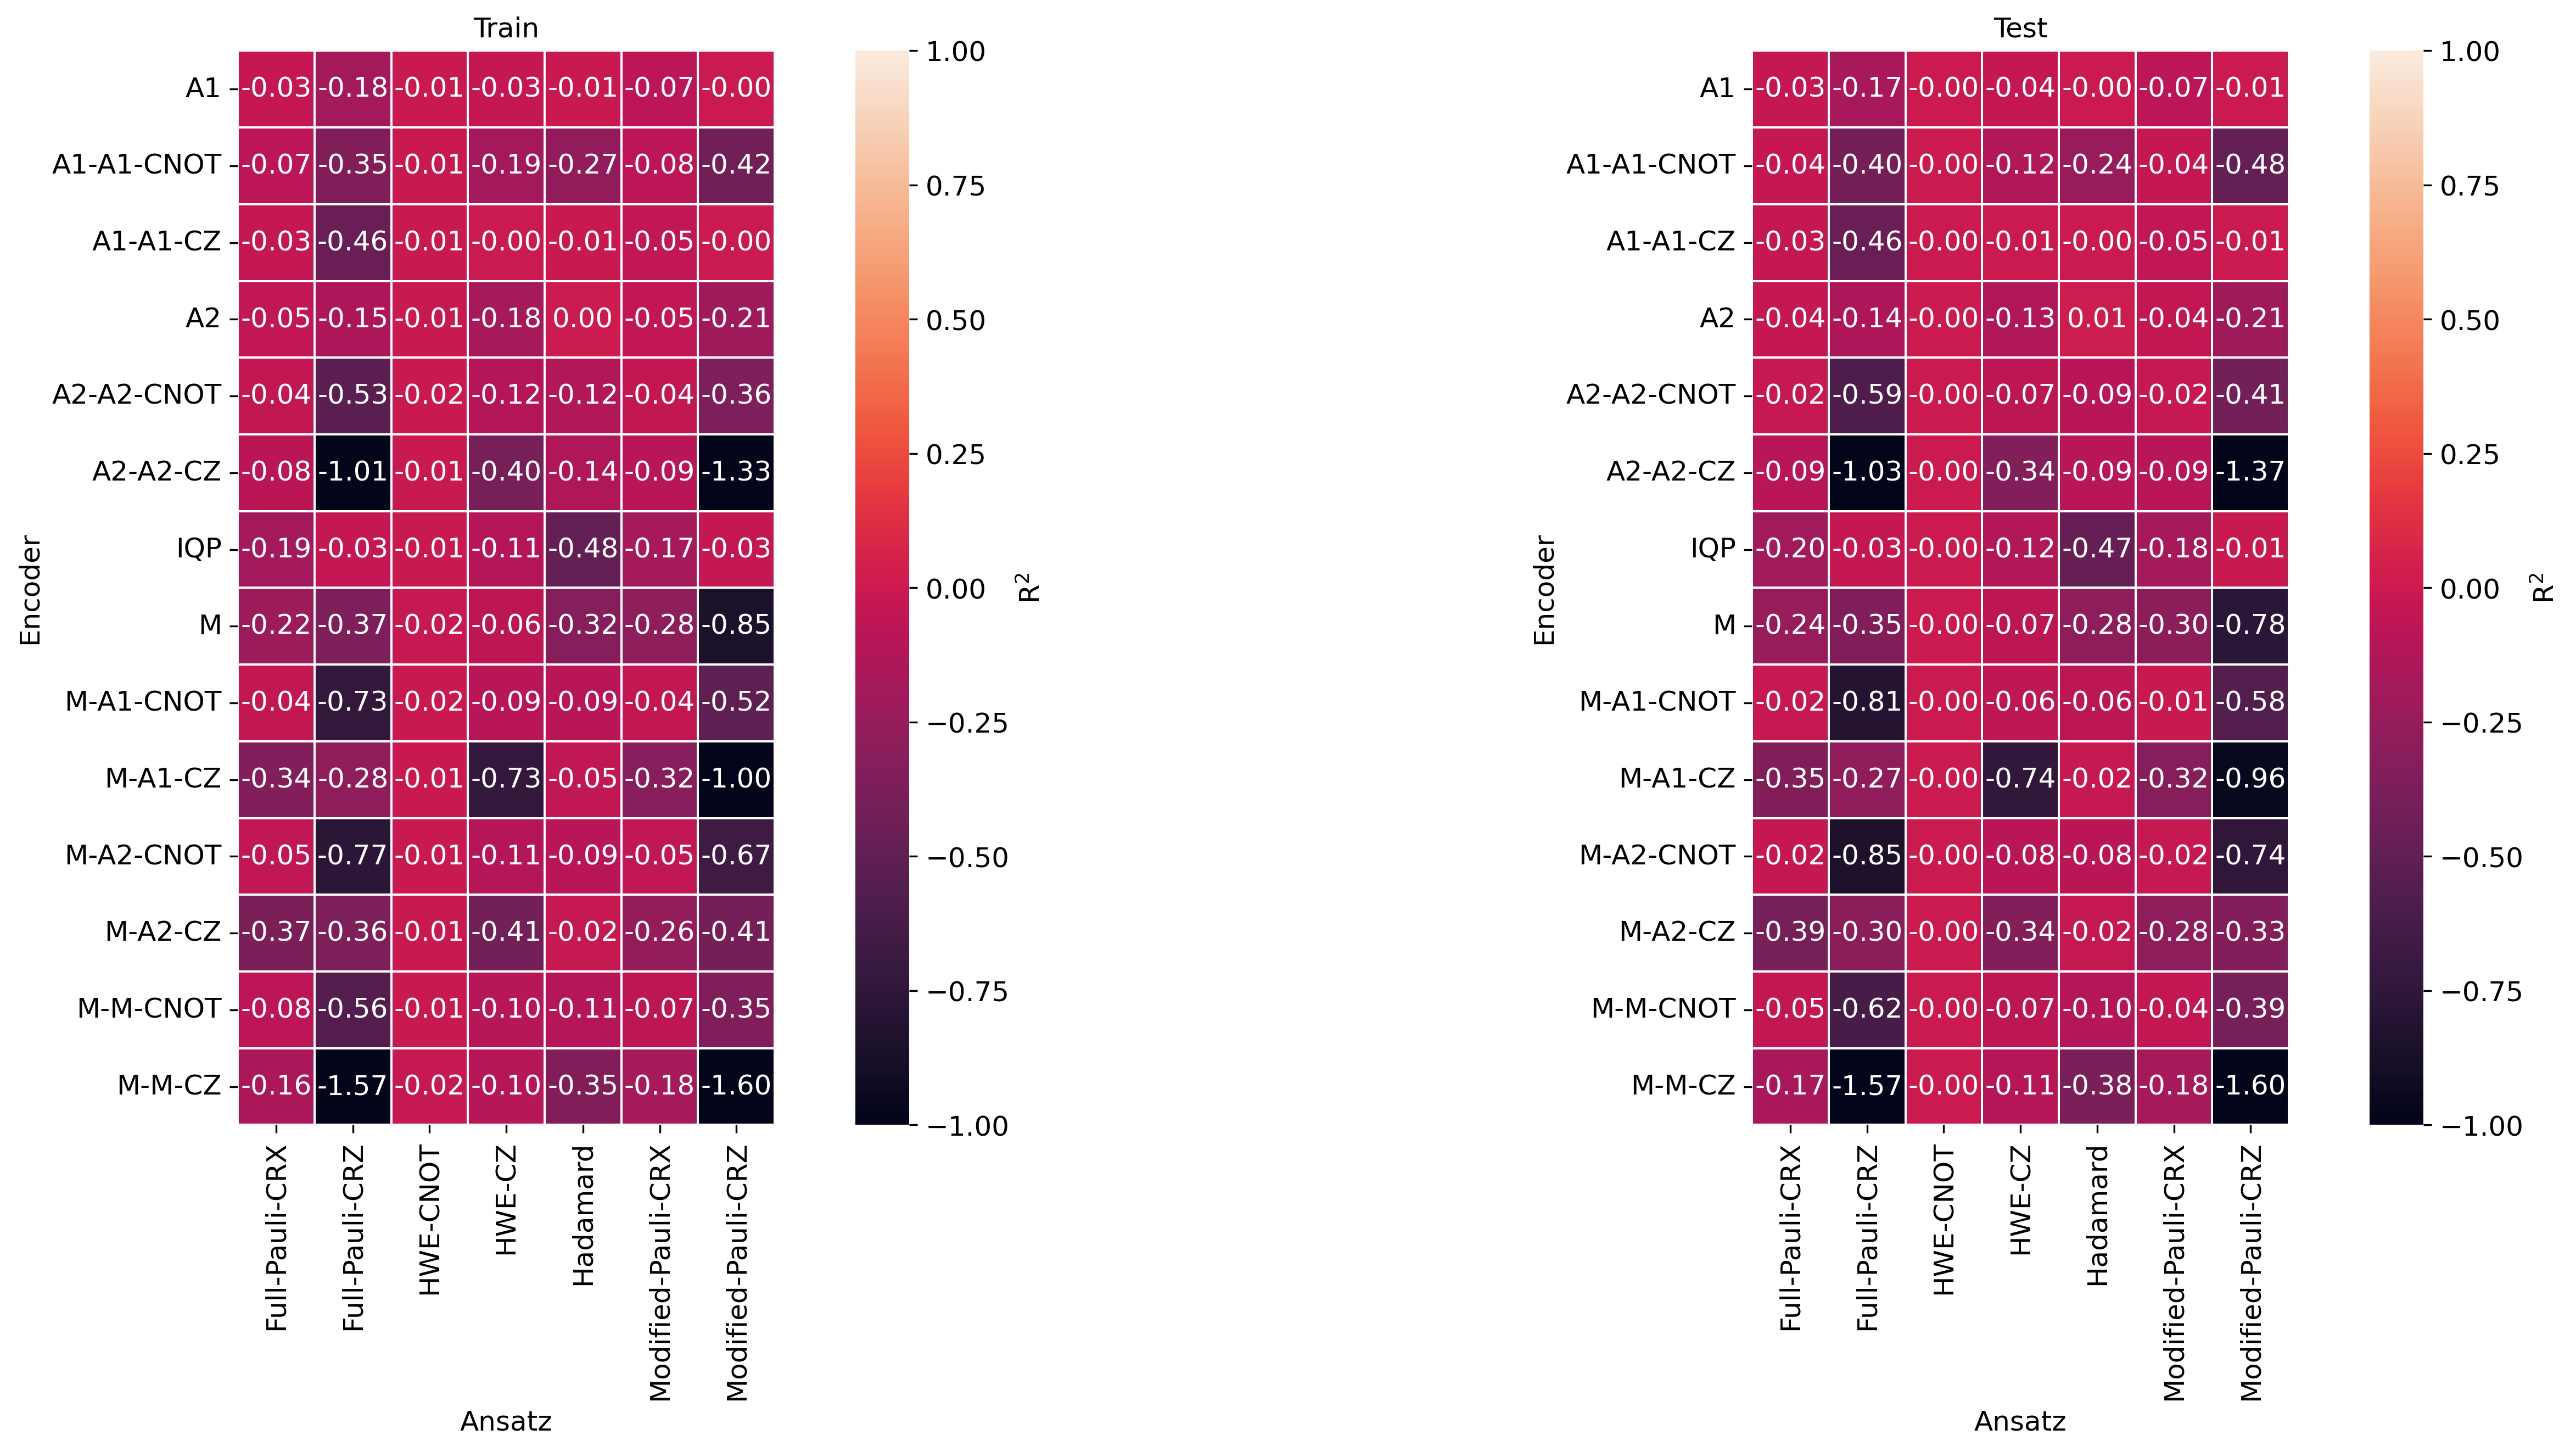
\includegraphics[width=\linewidth]{../images/BSE/sixteenqubit/BSE_heatplots}
		\caption{}
		\label{fig:16BSE_heatplots}
	\end{subfigure}
	\hfill
	\begin{subfigure}[b]{0.49\textwidth}
		\centering
		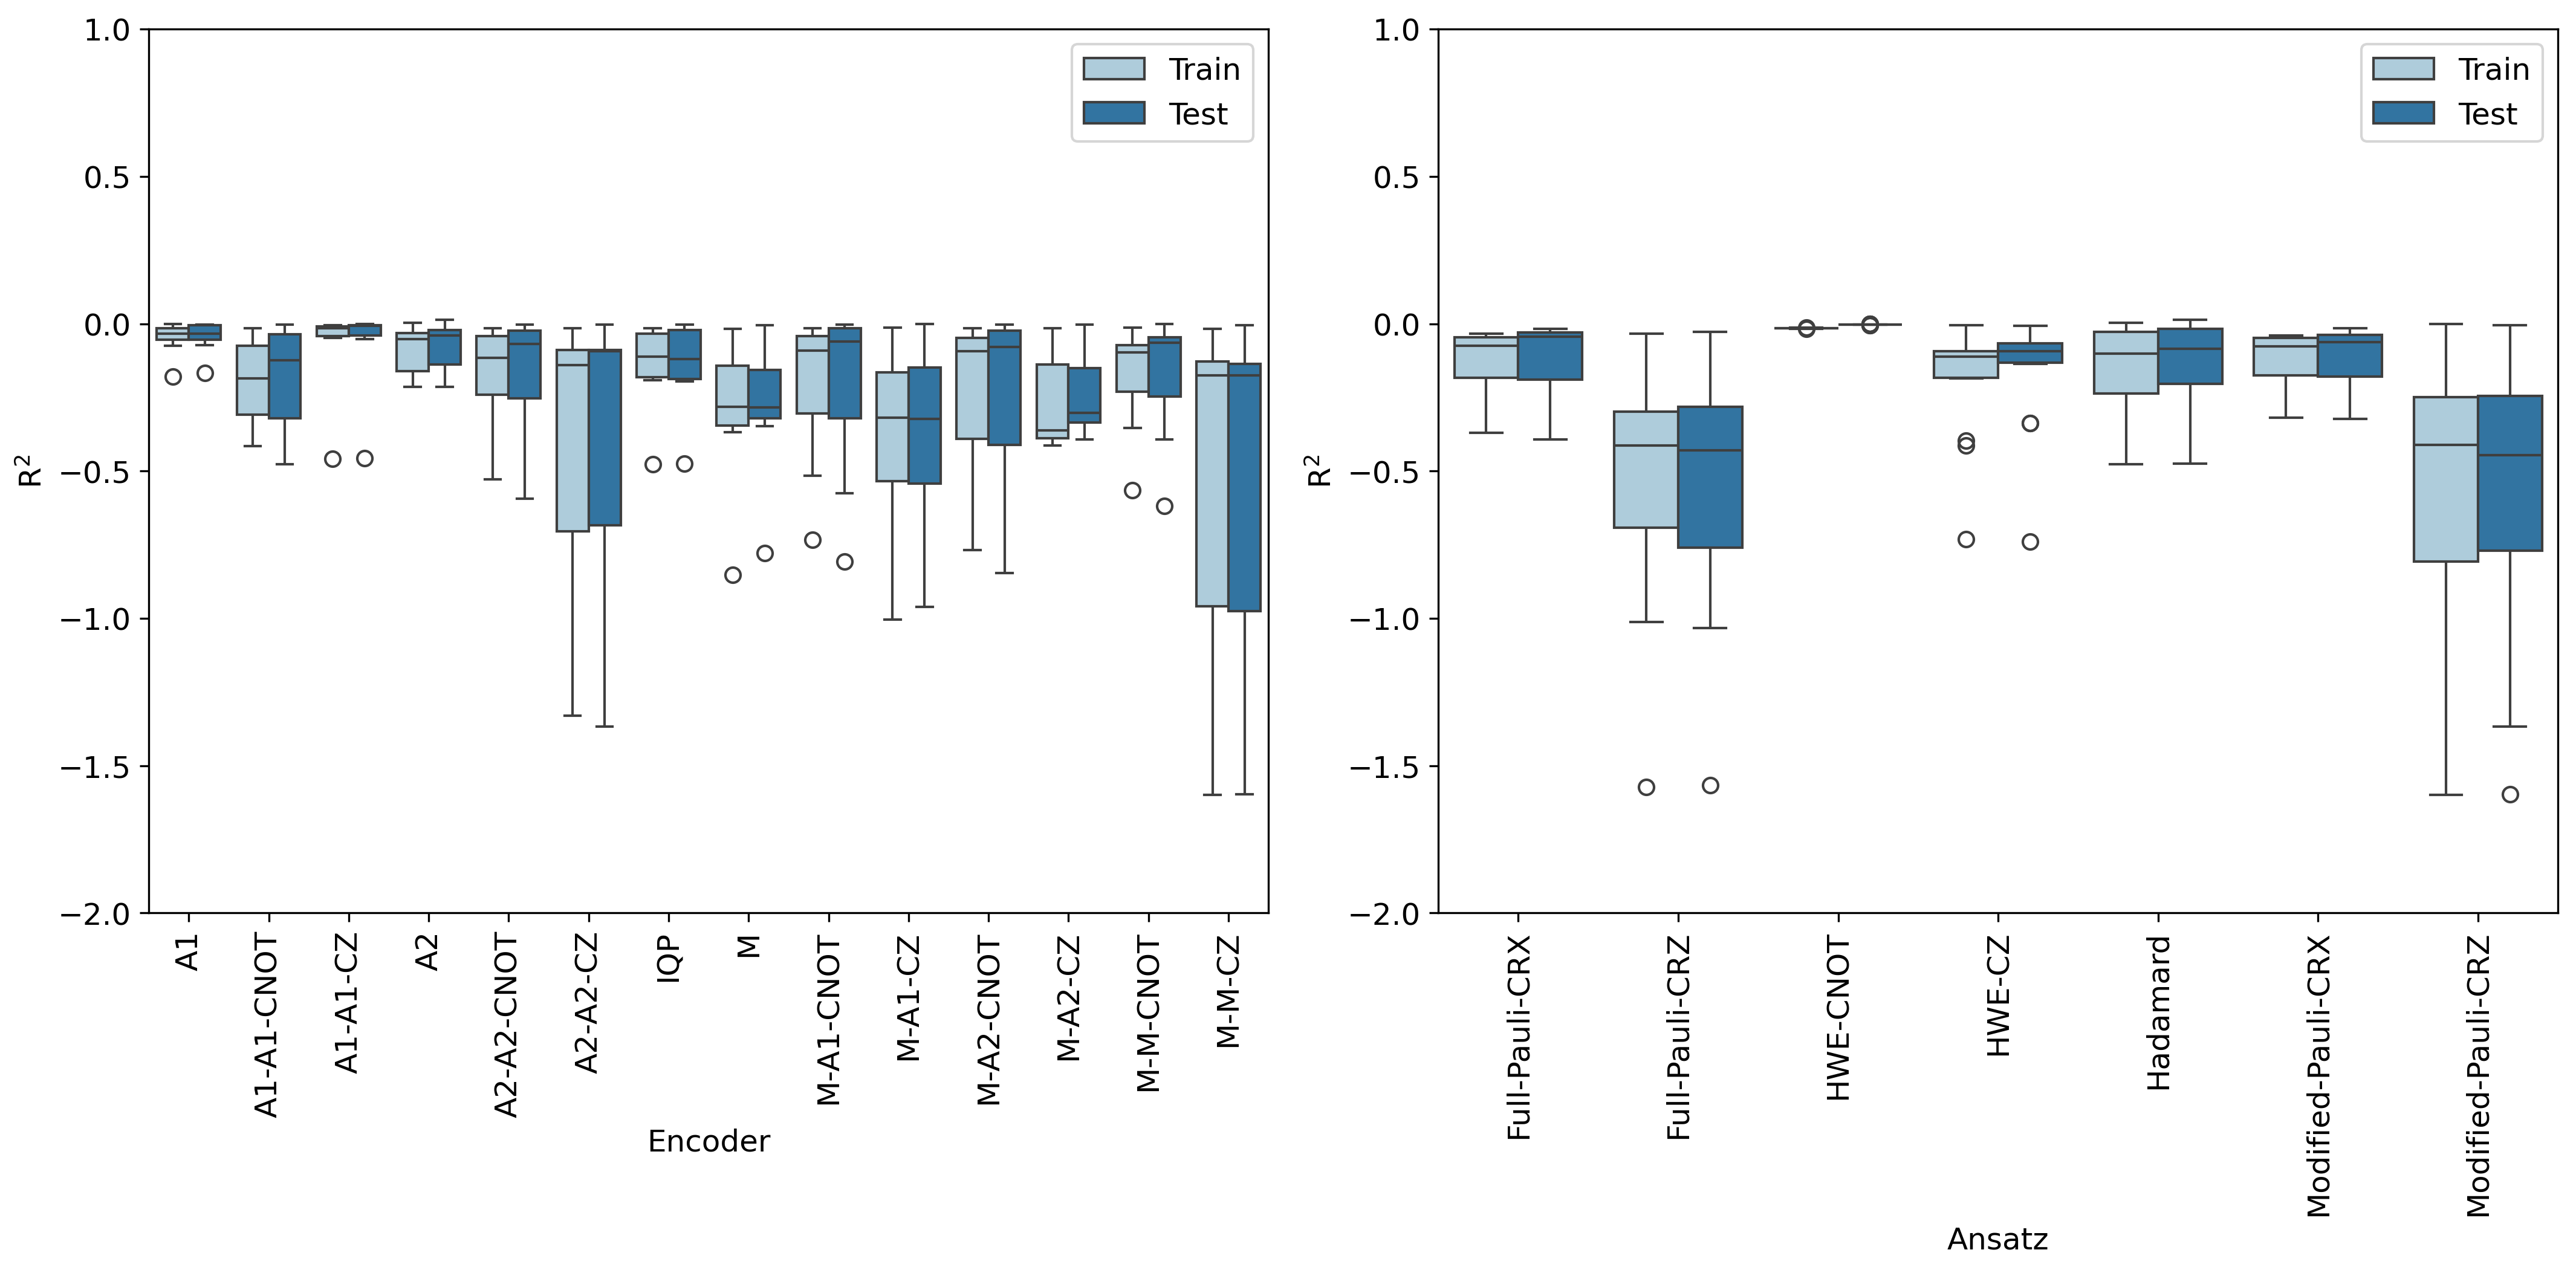
\includegraphics[width=\linewidth]{../images/BSE/sixteenqubit/BSE_boxplots}
		\caption{}
		\label{fig:16BSE_boxplots}
	\end{subfigure}
	\caption{}
	\label{fig:BSEboxandheat}	
\end{figure}

\begin{figure}[H]
	\centering	
	\begin{subfigure}[b]{0.49\textwidth}
		\centering
		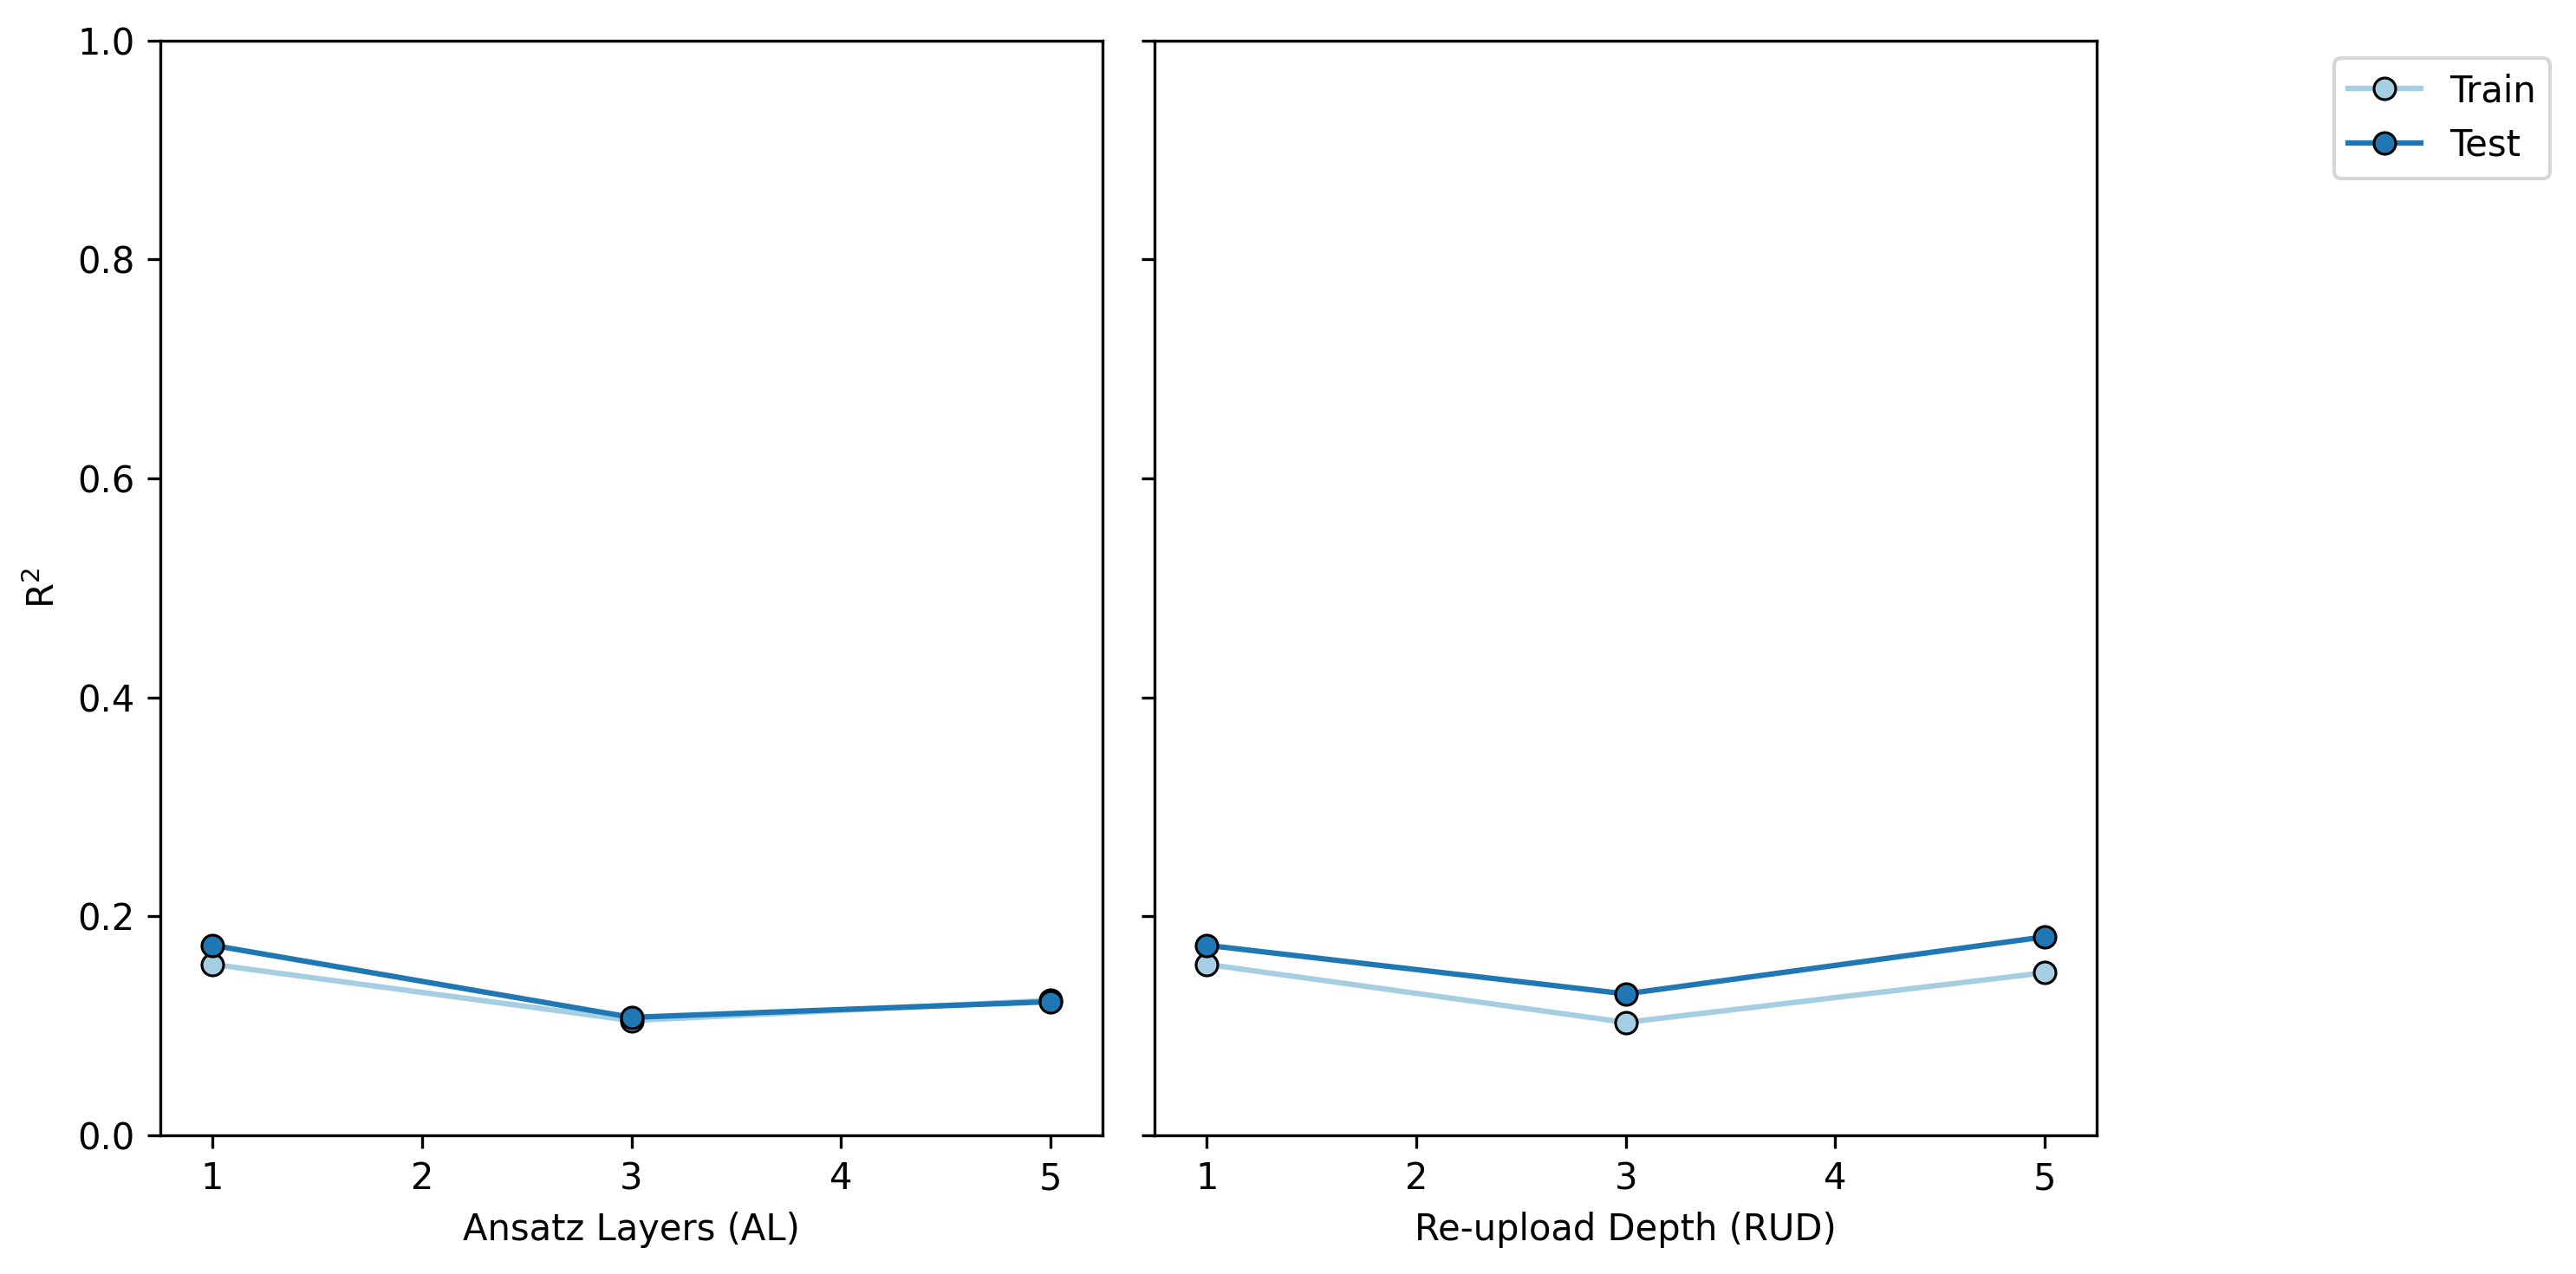
\includegraphics[width=\linewidth]{../images/BSE/fivequbit/BSE5_RUDAL_lineplot}
		\caption{}
		\label{fig:bse5RUDAL_lineplot}
	\end{subfigure}
	\hfill
	\begin{subfigure}[b]{0.49\textwidth}
		\centering
		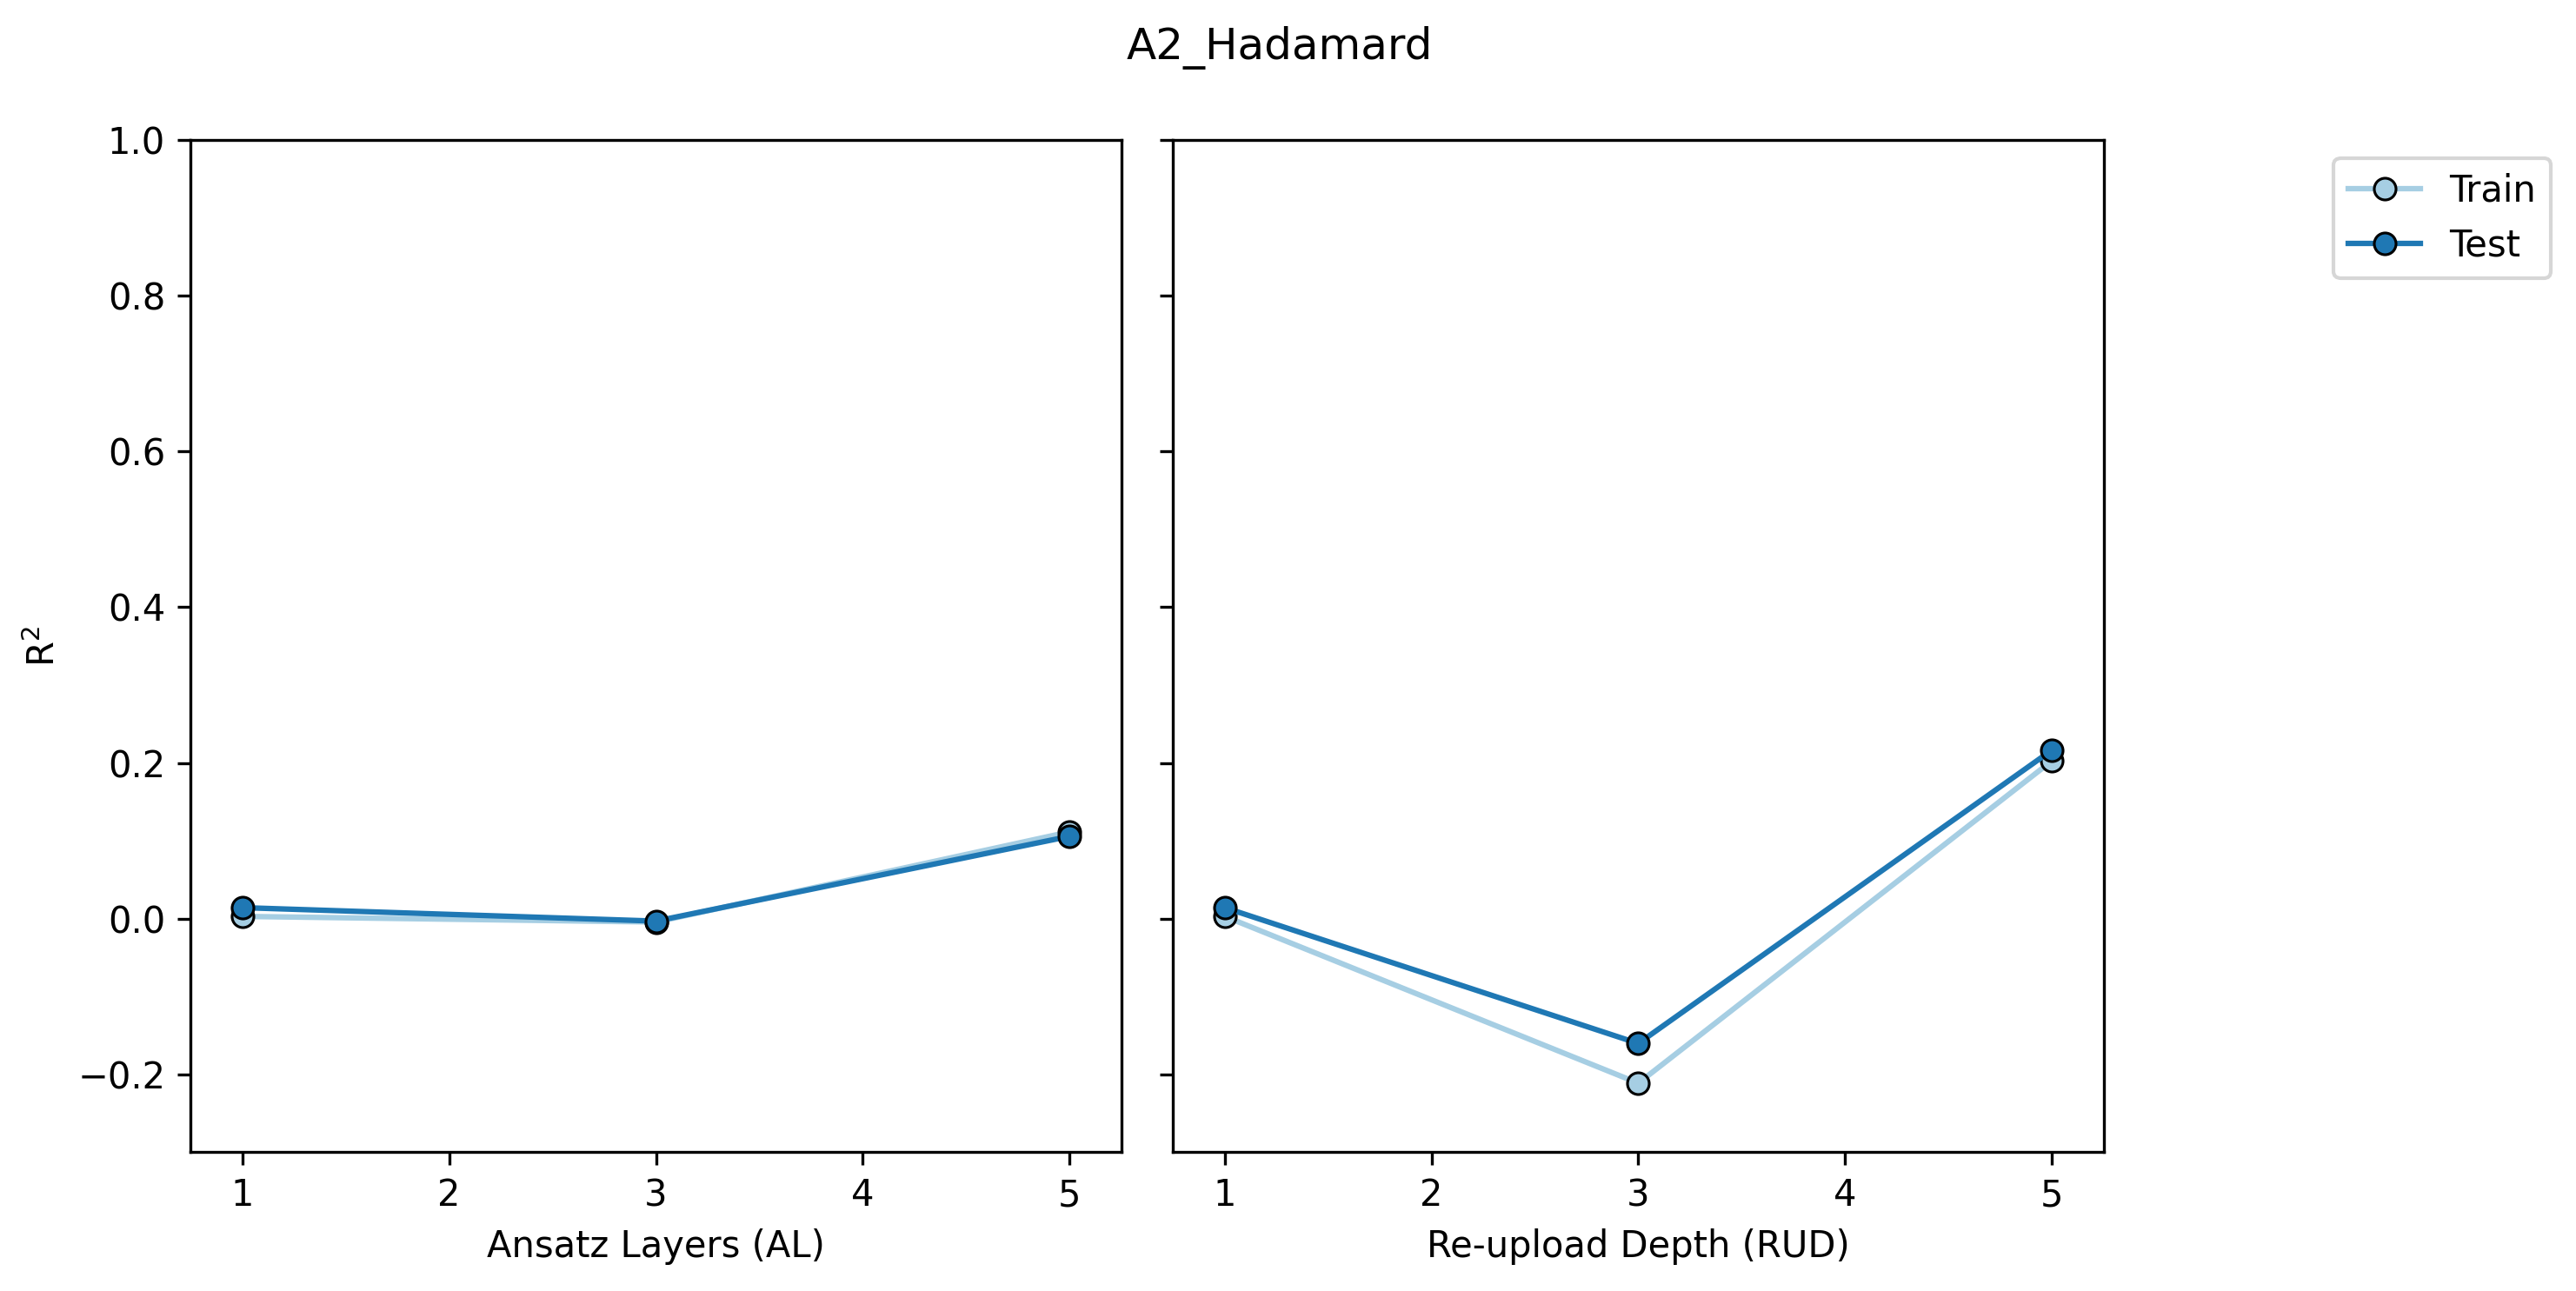
\includegraphics[width=\linewidth]{../images/BSE/sixteenqubit/BSE16_RUDAL_lineplot}
		\caption{}
		\label{fig:bse16RUDAL_lineplot}
	\end{subfigure}
	\hfill
	\begin{subfigure}[b]{\textwidth}
		\centering
		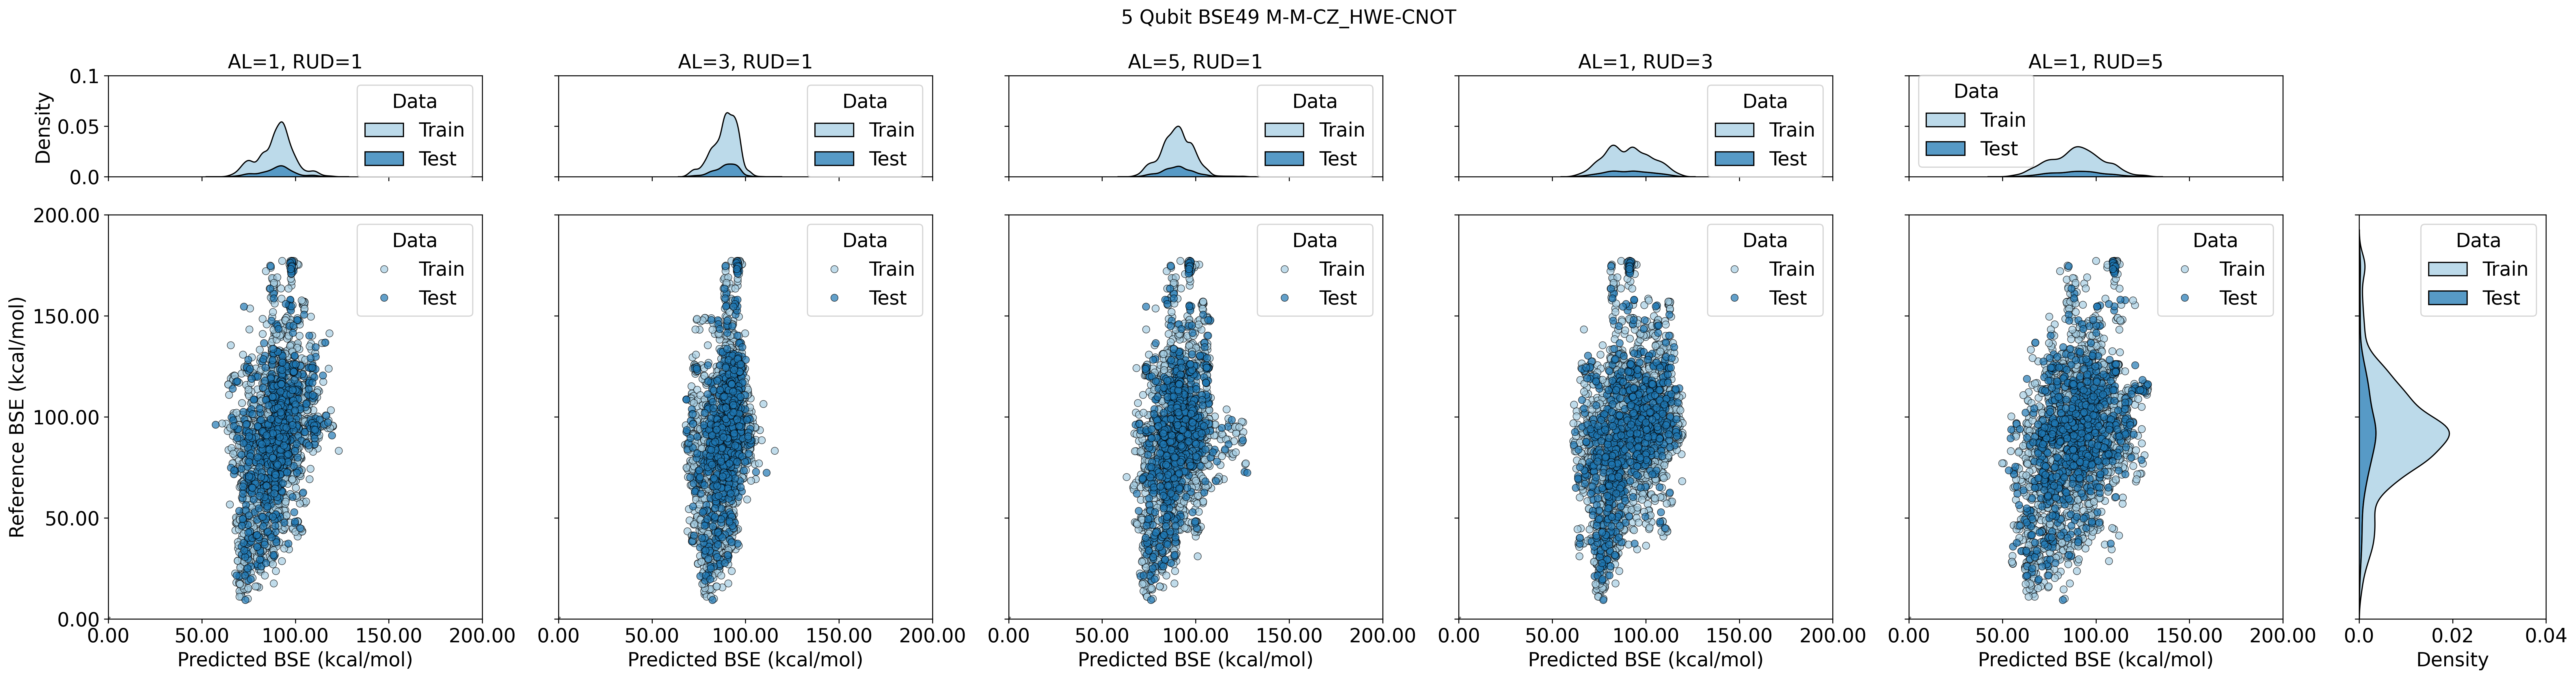
\includegraphics[width=\linewidth]{../images/BSE/fivequbit/distribution_parity}
		\caption{}
		\label{fig:BSE5_distribution_parity}
	\end{subfigure}
	\hfill
	\begin{subfigure}[b]{\textwidth}
		\centering
		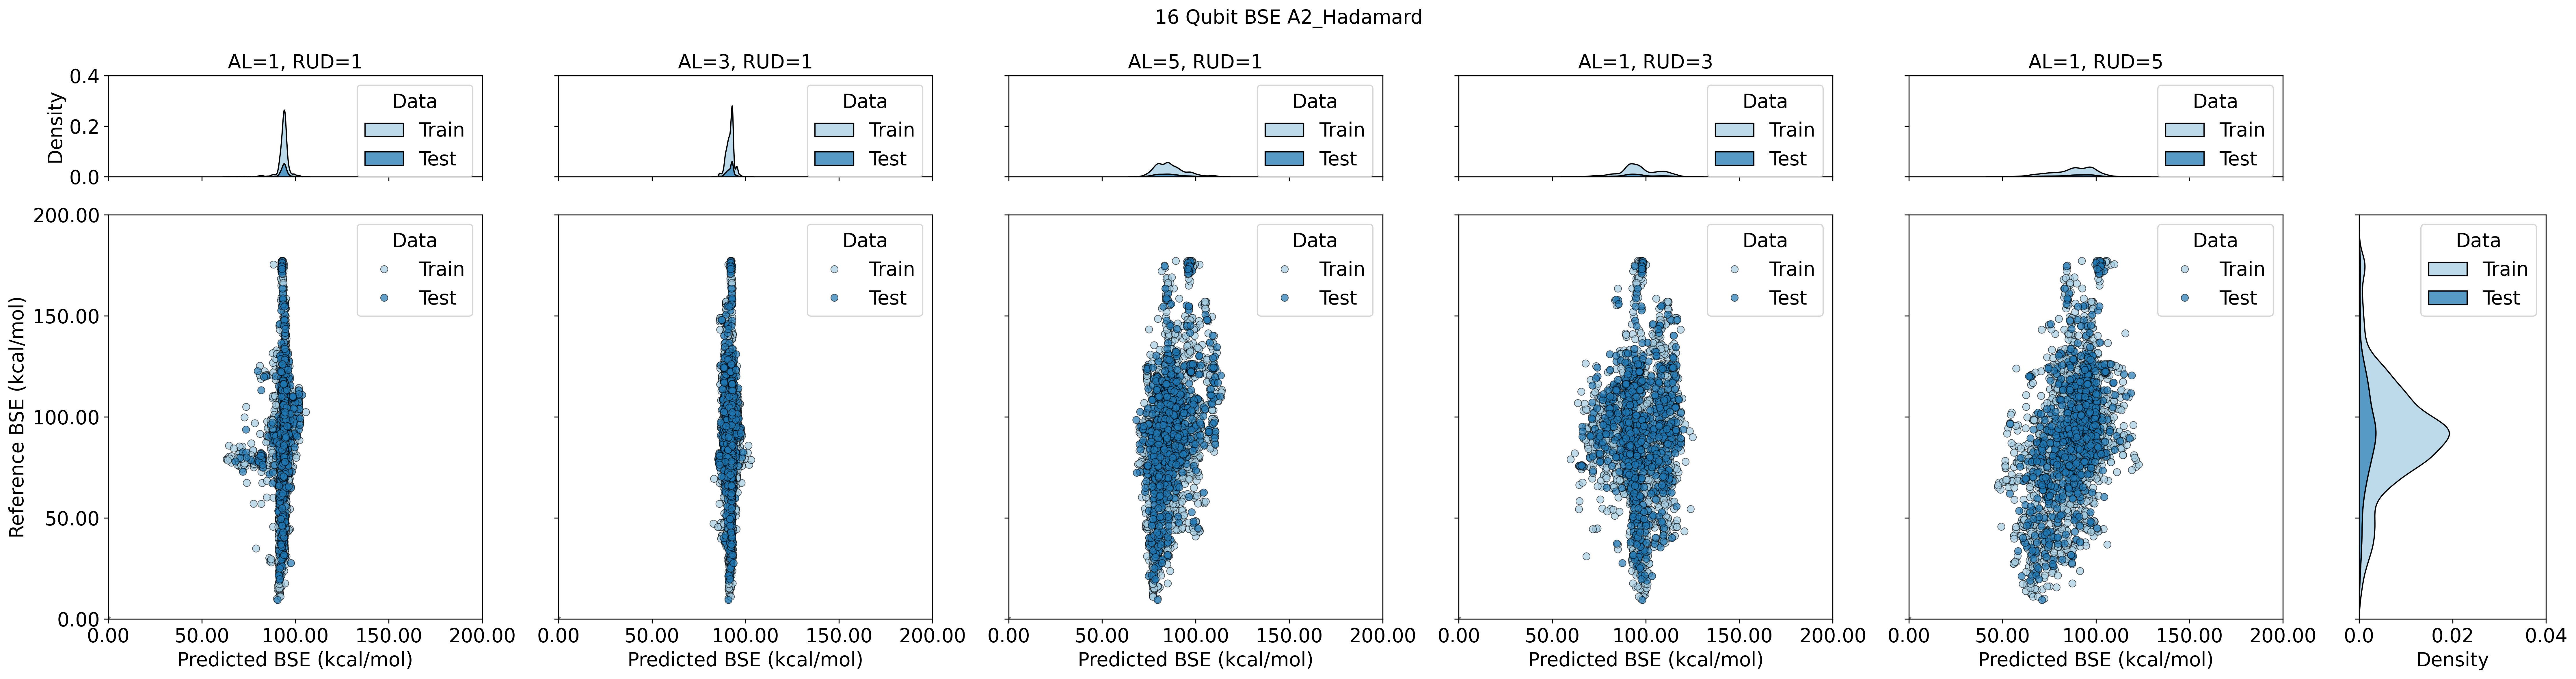
\includegraphics[width=\linewidth]{../images/BSE/sixteenqubit/distribution_parity}
		\caption{}
		\label{fig:BSE16_distribution_parity}
	\end{subfigure}
	\caption{}
	\label{fig:BSE_distribution_parity}	
\end{figure}



\begin{figure}[H]
	\centering	
	\begin{subfigure}[b]{0.49\textwidth}
		\centering
		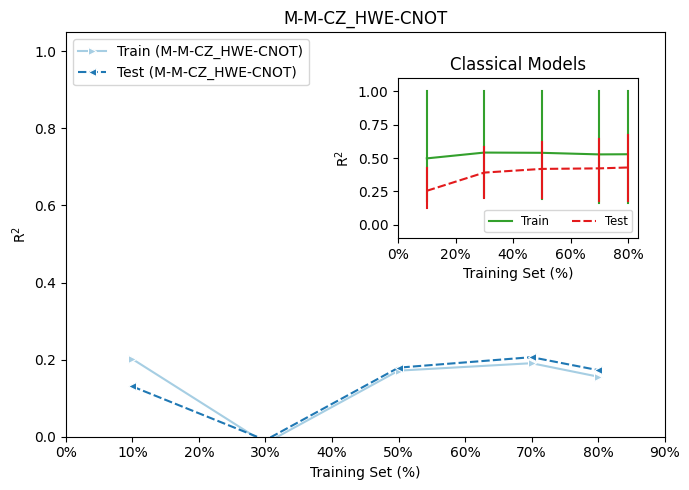
\includegraphics[width=\linewidth]{../images/BSE/fivequbit/BSE_learningcurve}
		\caption{}
		\label{fig:BSE5_learning_curves}
	\end{subfigure}
	\hfill
	\begin{subfigure}[b]{0.49\textwidth}
		\centering
		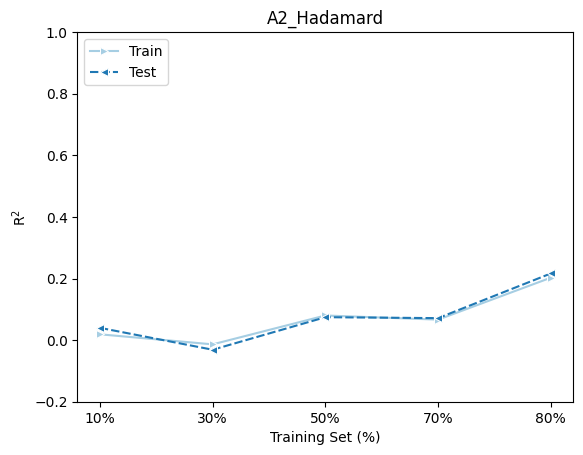
\includegraphics[width=\linewidth]{../images/BSE/sixteenqubit/BSE_learningcurve}
		\caption{}
		\label{fig:BSE16_learningcurve}
	\end{subfigure}
	\caption{}
	\label{fig:BSE_LC}	
\end{figure}







\subsection{DDCC}


A2\_HWE-CNOT Train R$^{2}$ 0.62/test R$^{2}$ 0.62 
Best encoder average Train R$^{2}$ X/test R$^{2}$ Y
Best ansatz HWE-CNOT average Train R$^{2}$ X/test R$^{2}$ Y

\begin{figure}[H]
	\centering	
	\begin{subfigure}[b]{0.49\textwidth}
		\centering
		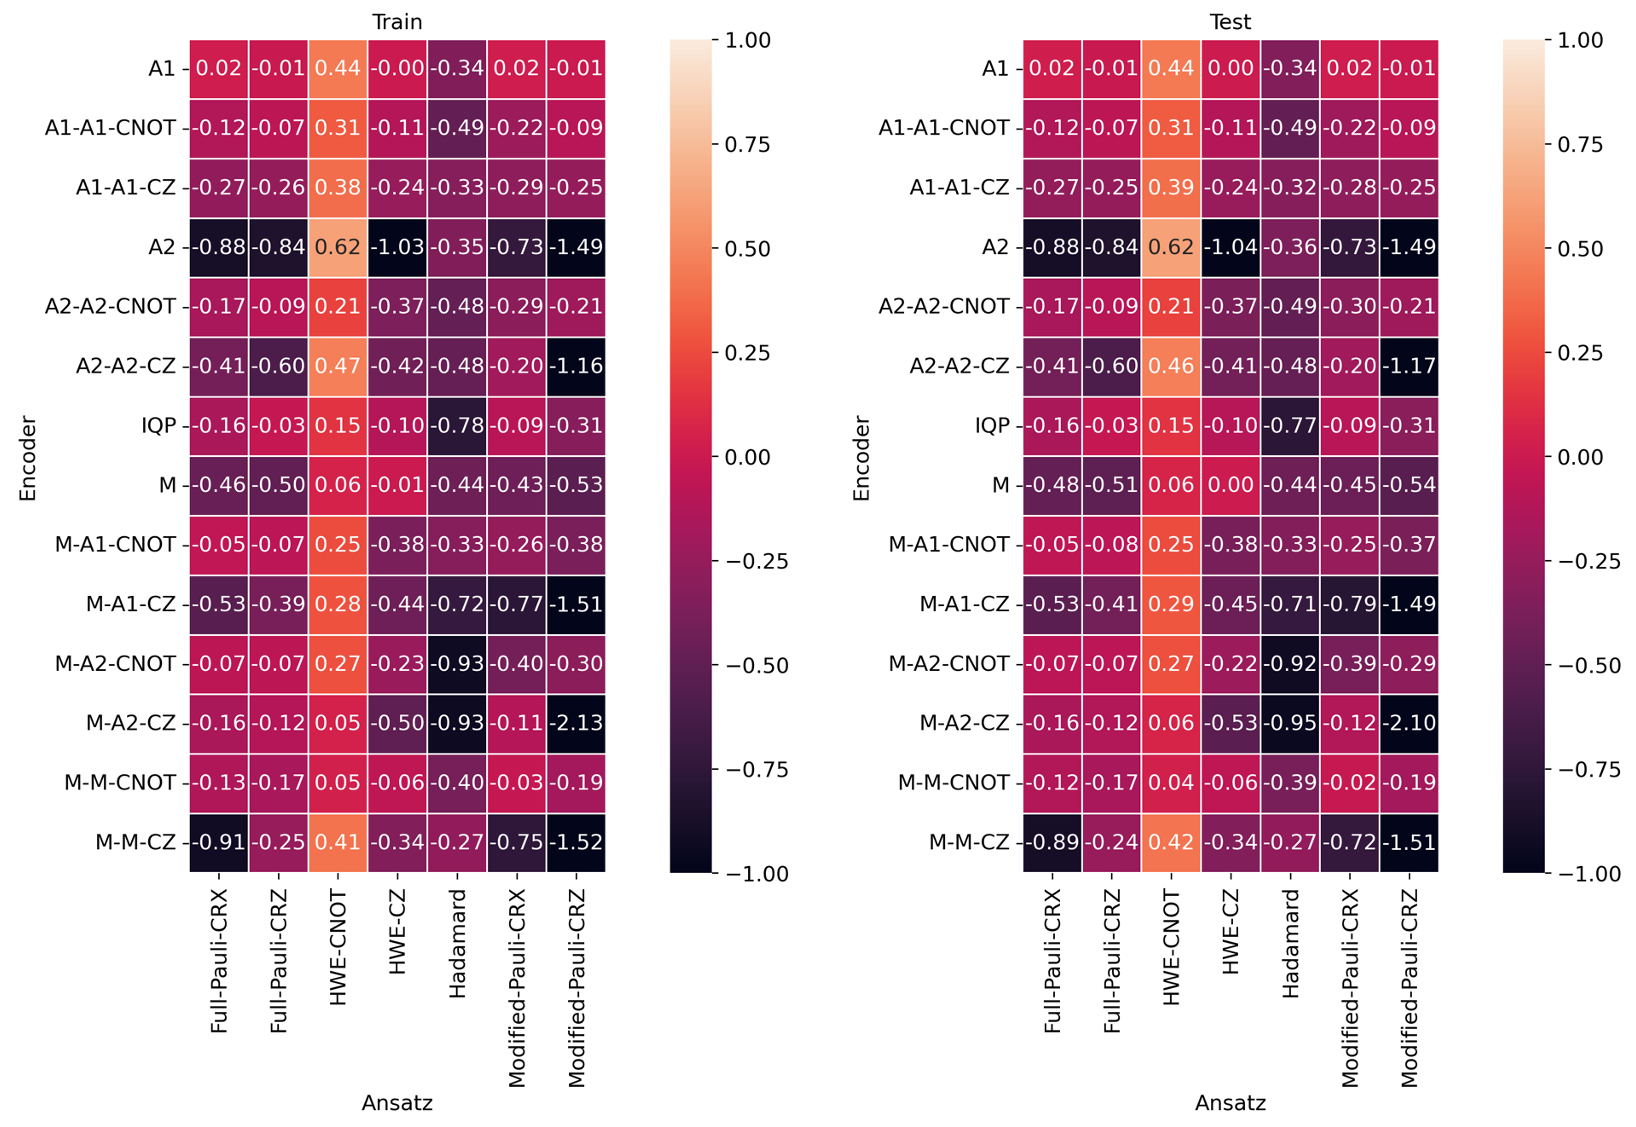
\includegraphics[width=\linewidth]{../images/DDCC/DDCC_heatplots}
		\caption{}
		\label{fig:ddccheatplots}
	\end{subfigure}
	\hfill	
	\begin{subfigure}[b]{0.49\textwidth}
		\centering
		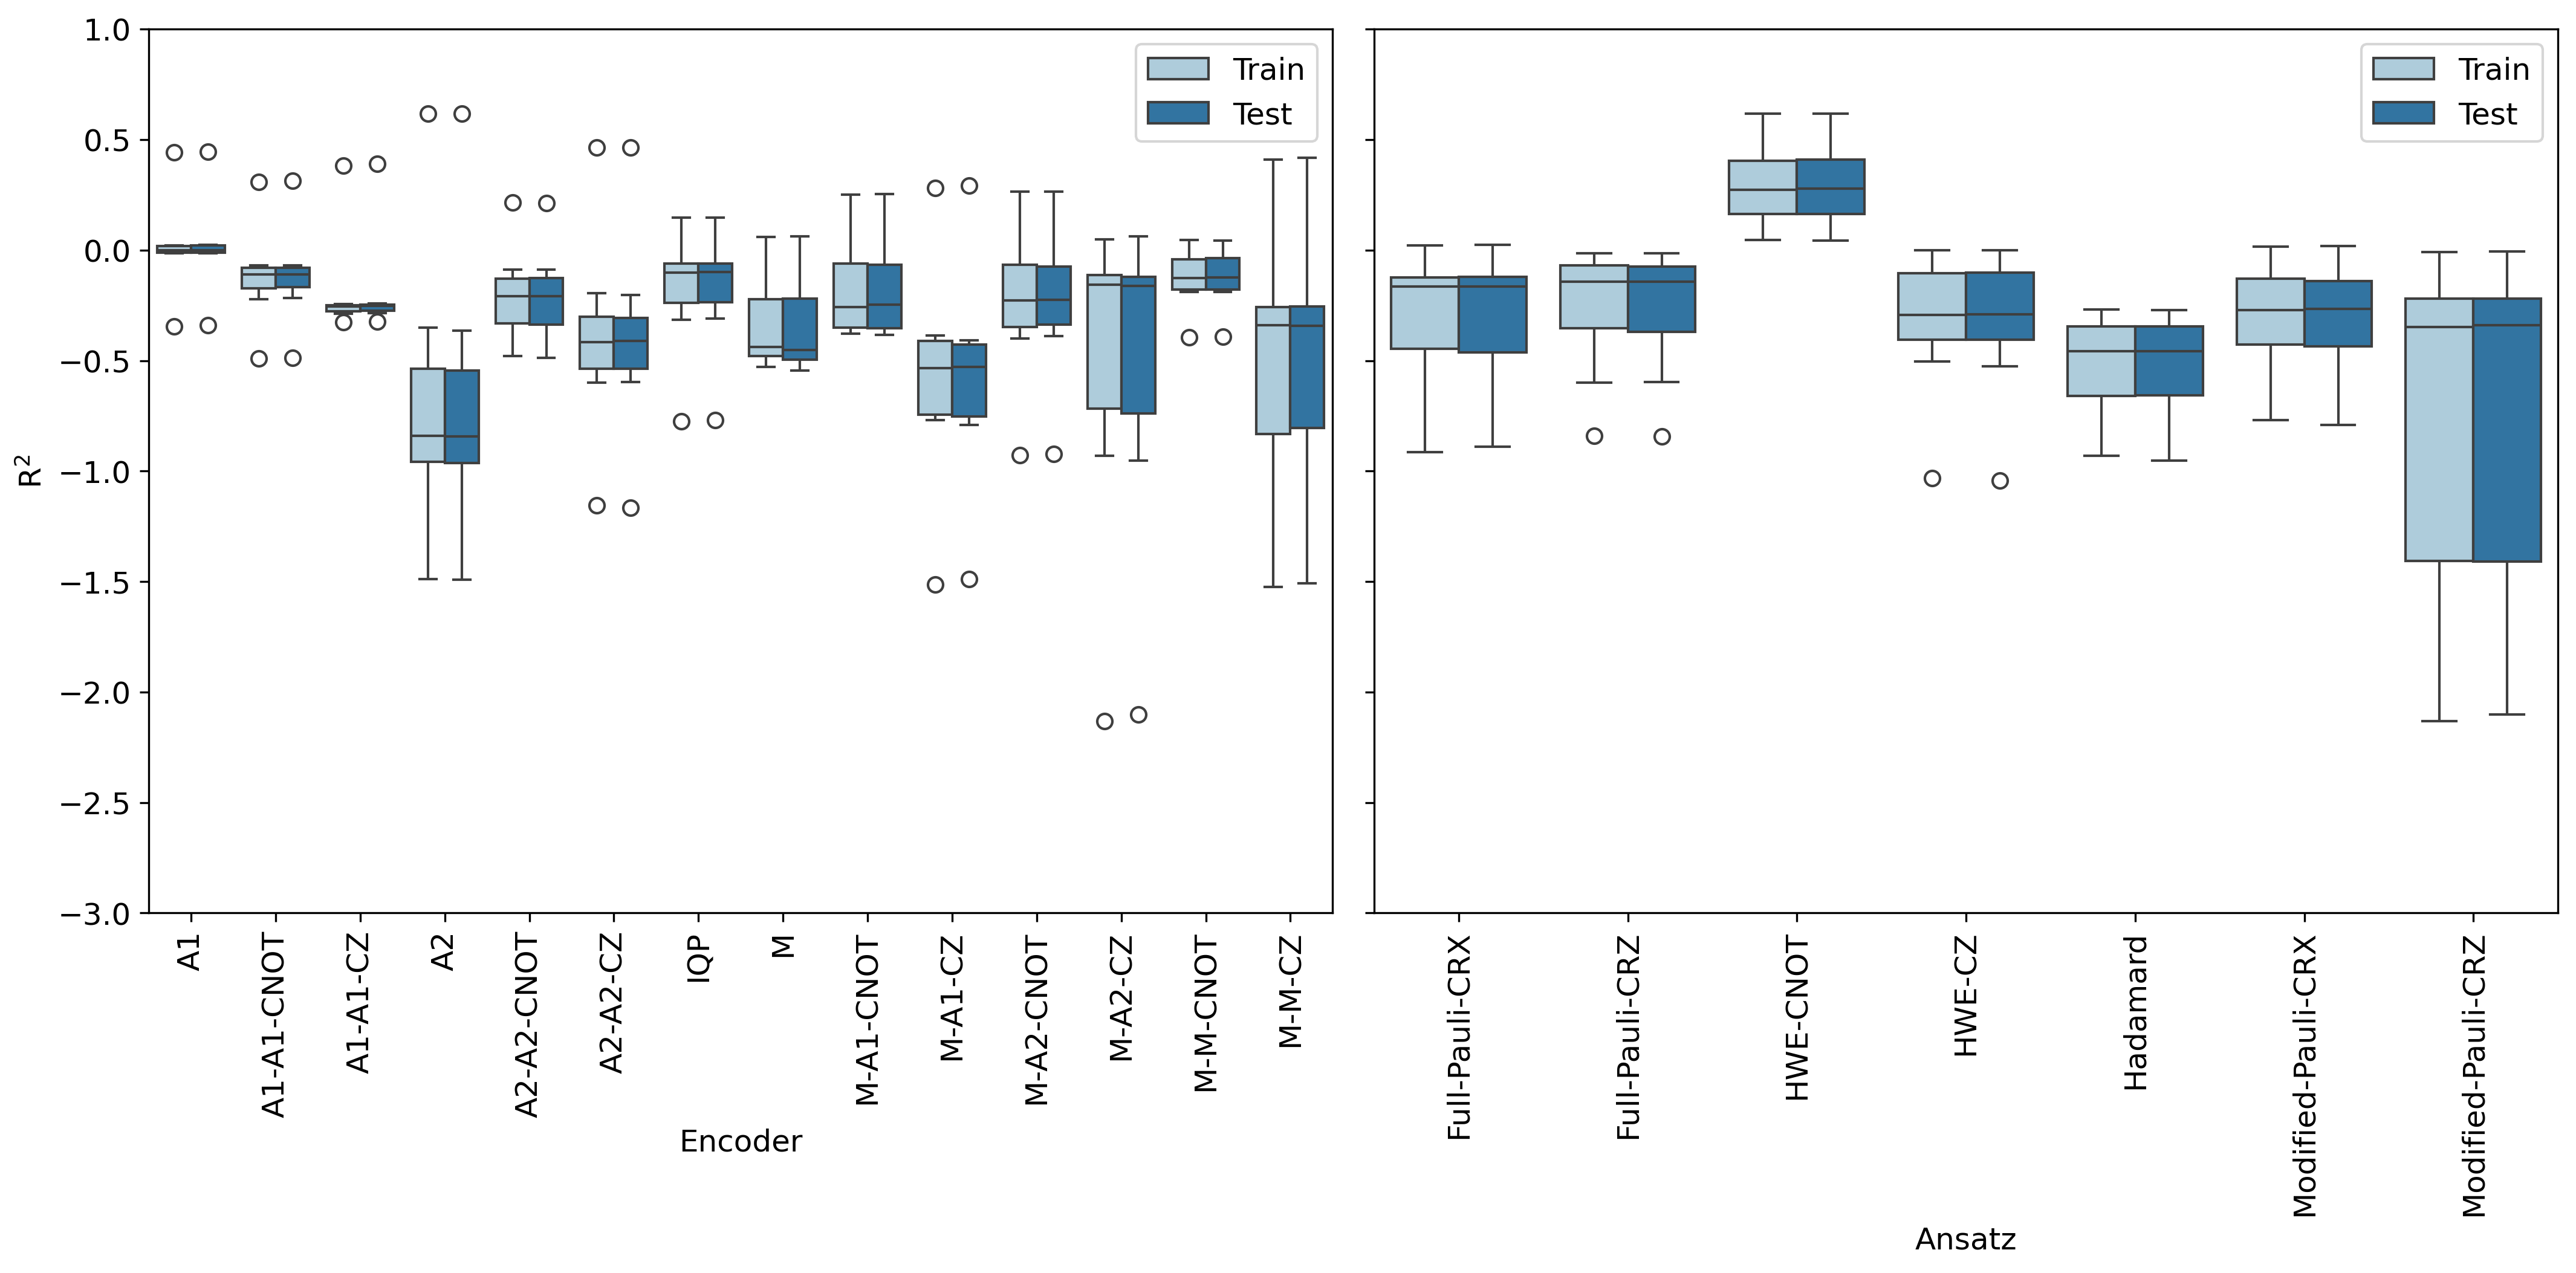
\includegraphics[width=\linewidth]{../images/DDCC/DDCC_boxplots}
		\caption{}
		\label{fig:ddccboxplots}
	\end{subfigure}
	\hfill
%	\begin{subfigure}[b]{0.49\textwidth}
%		\centering
%		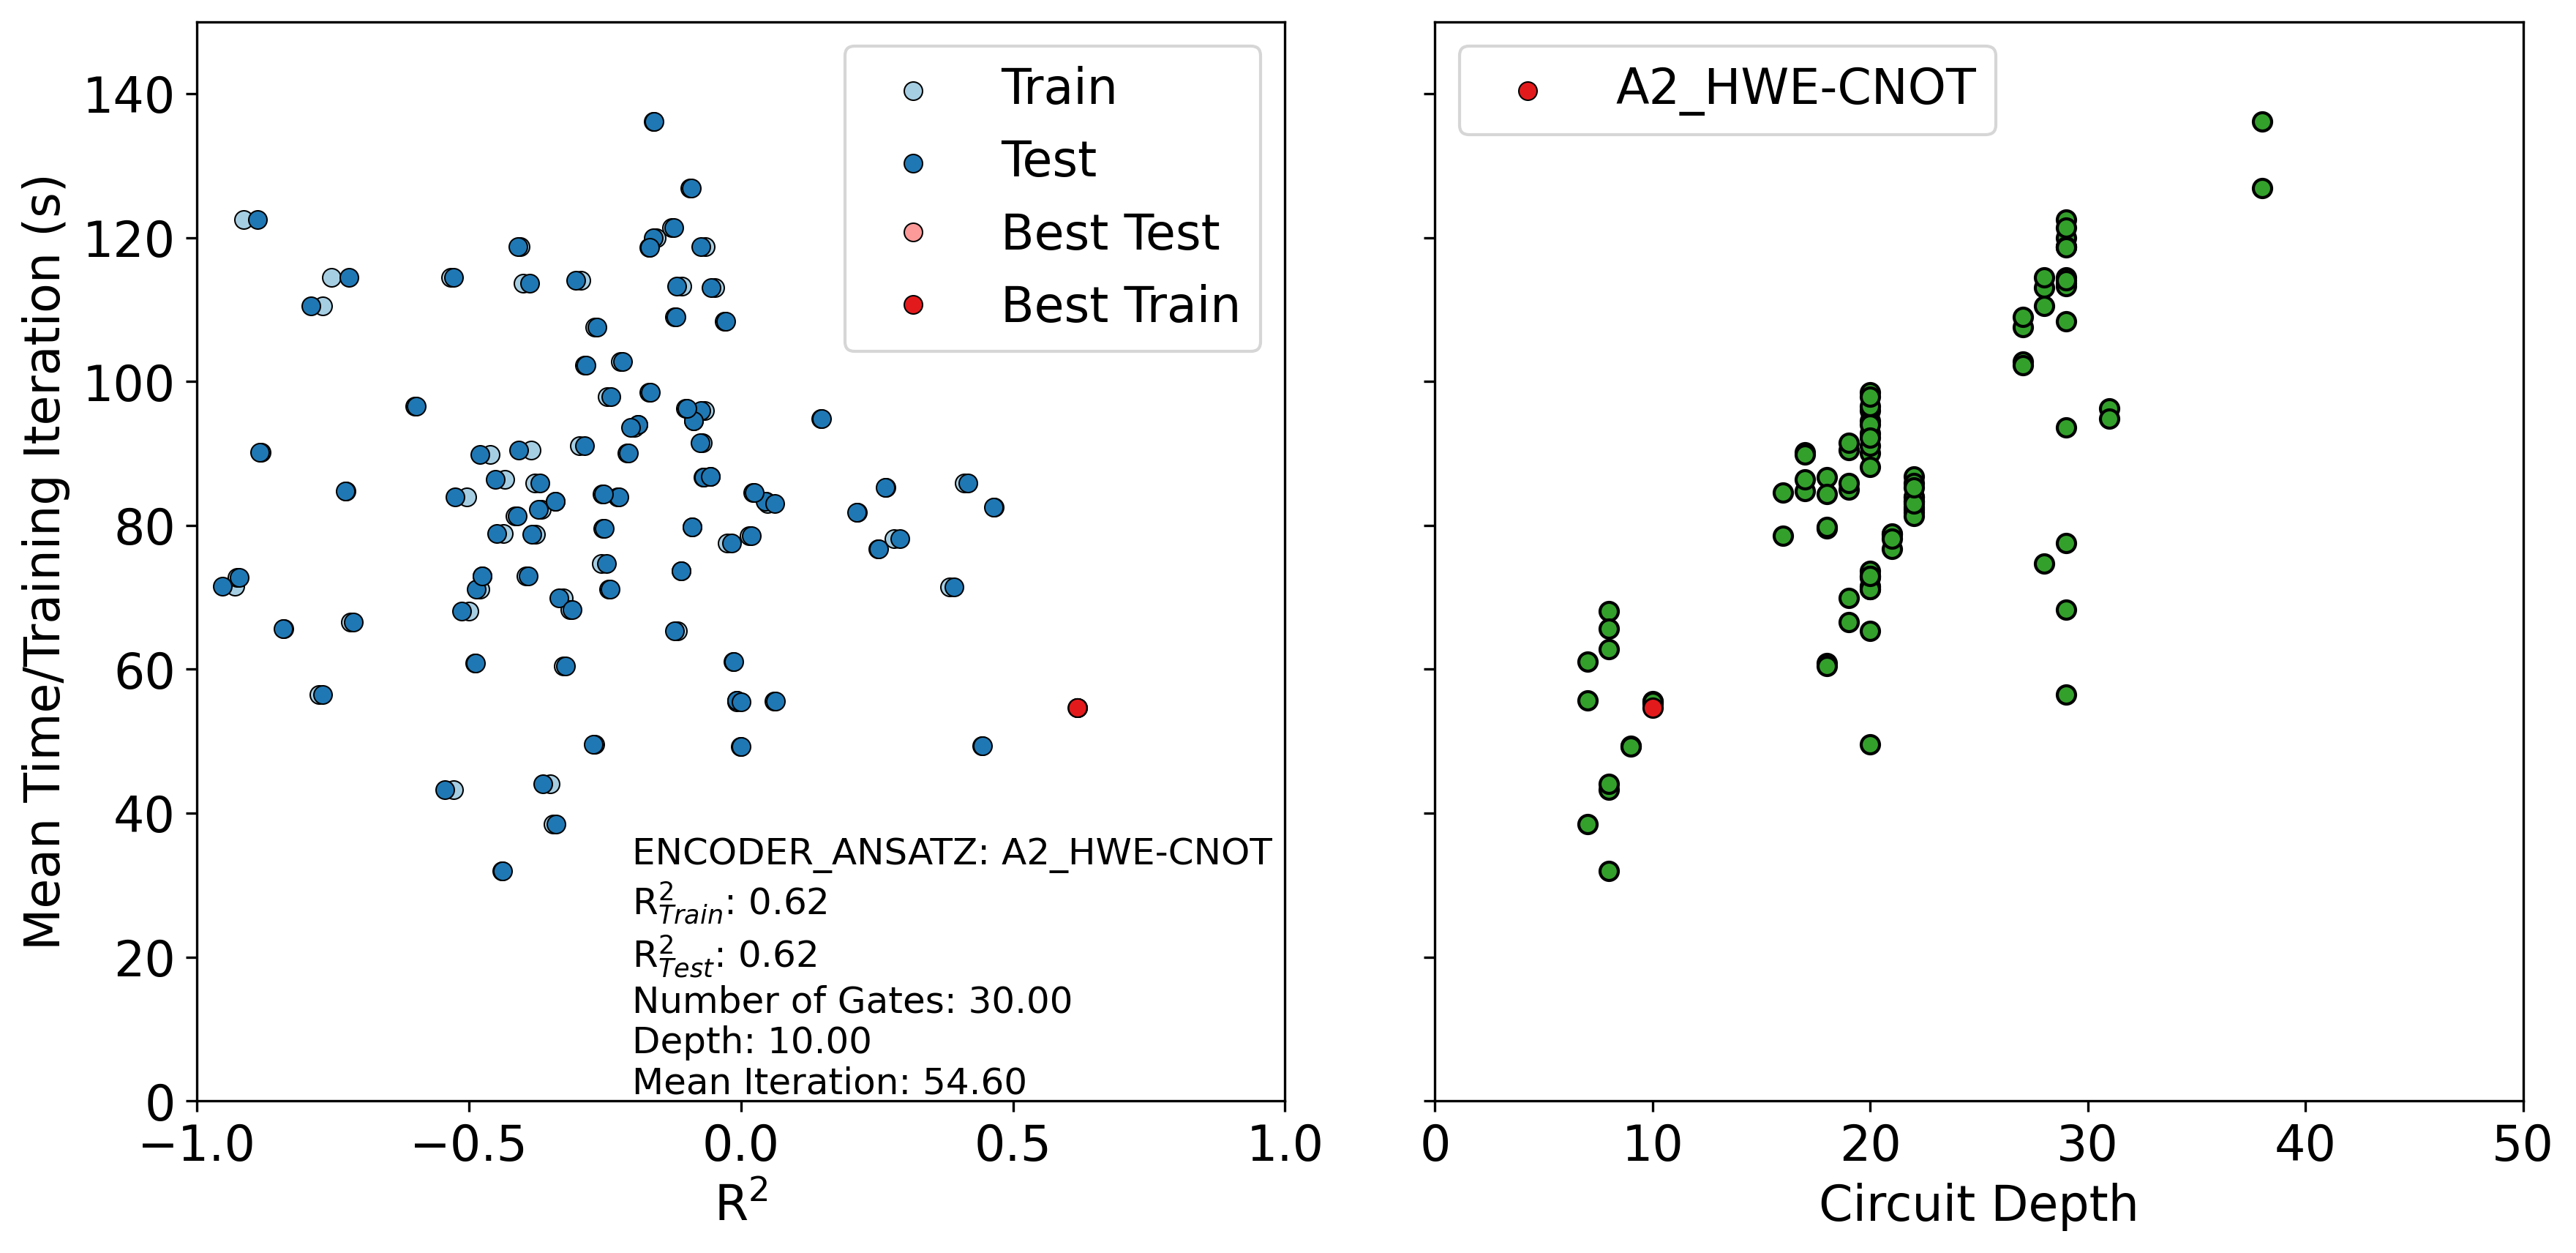
\includegraphics[width=\linewidth]{../images/DDCC/AllDDCC5_circuitdepth_R2_vs_iterationtime}
%		\caption{}
%		\label{fig:allddcc5circuitdepthr2vsiterationtime}
%	\end{subfigure}	
	\caption{}
	\label{fig:ddcc_all_analysis}	
\end{figure}


(AL,RUD)=(1,1) Train R$^{2}$ 0.62/test R$^{2}$ 0.62
(AL,RUD)=(1,3) Train R$^{2}$ 0.85/test R$^{2}$ 0.85
(AL,RUD)=(1,5) Train R$^{2}$ 0.82/test R$^{2}$ 0.83
(AL,RUD)=(3,1) Train R$^{2}$ 0.71/test R$^{2}$ 0.71
(AL,RUD)=(5,1) Train R$^{2}$ 0.77/test R$^{2}$ 0.77



\begin{figure}[H]
	\centering	
	\begin{subfigure}[b]{0.49\textwidth}
		\centering
		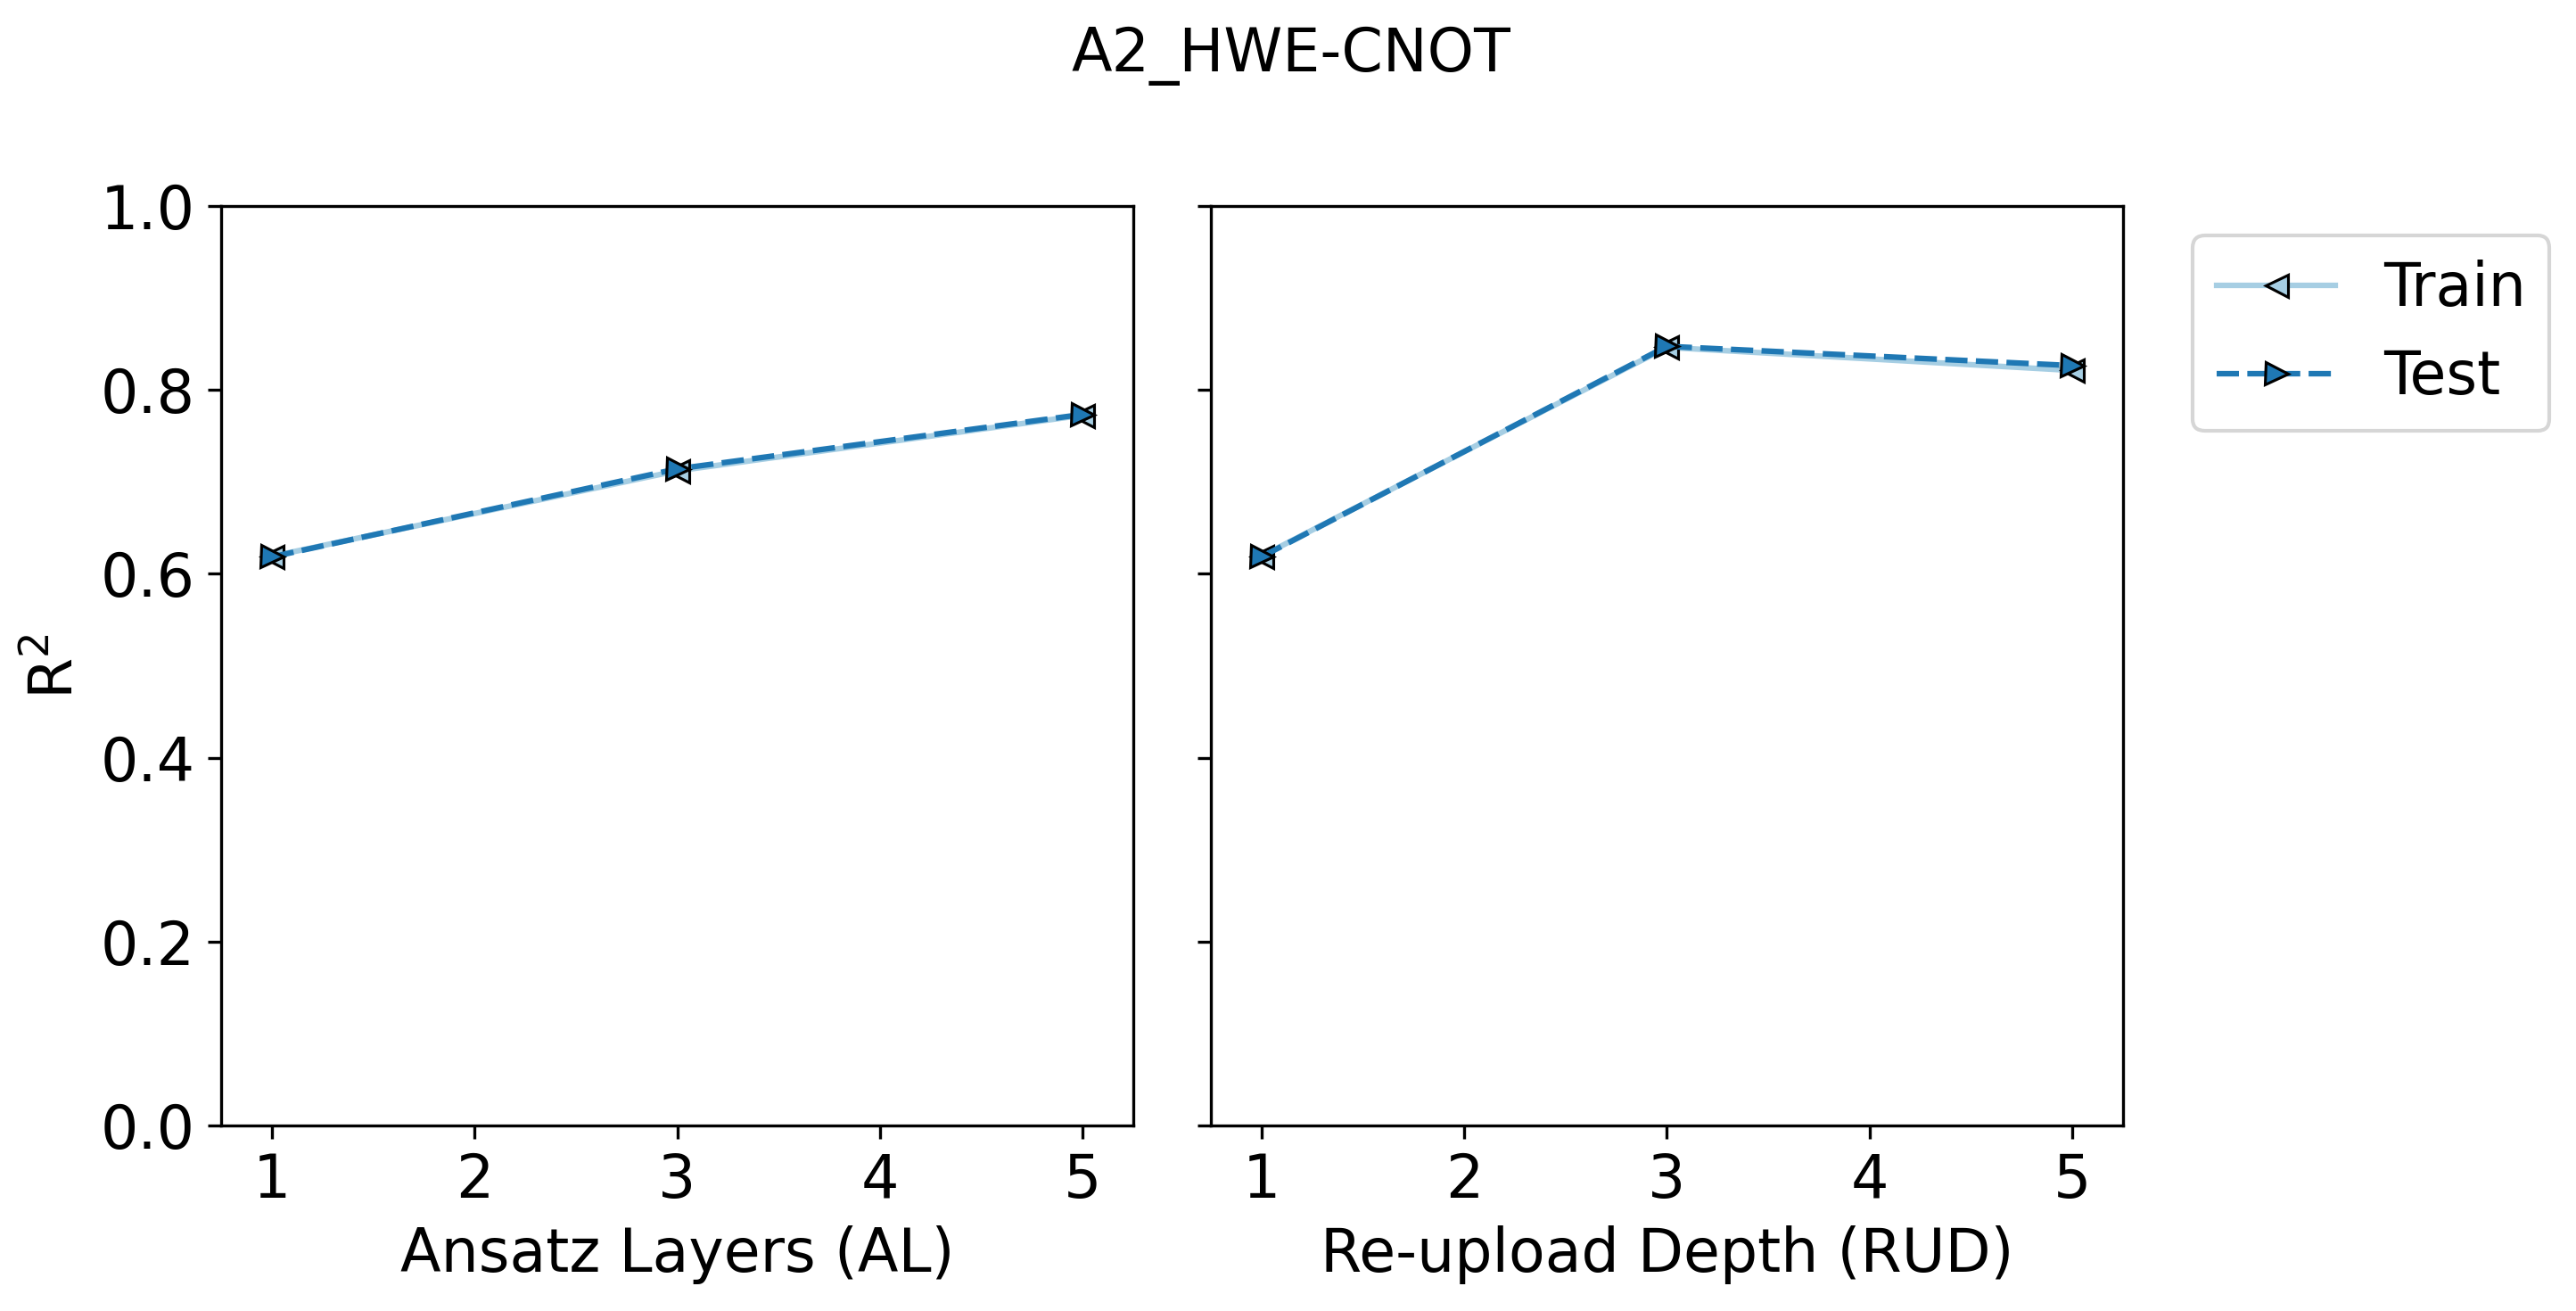
\includegraphics[width=\linewidth]{../images/DDCC/DDCC_RUDAL_lineplot}
		\caption{}
		\label{fig:ddccRUDAL_lineplot}
	\end{subfigure}
	\hfill
	\begin{subfigure}[b]{\textwidth}
		\centering
		\includegraphics[width=\linewidth]{../images/DDCC/distribution_parity}
		\caption{}
		\label{fig:ddccdistribution_parity}
	\end{subfigure}
	\caption{Model evaluation, using R$^{2}$ (y-axis), of re-upload depths (RUD) and ansatz layers (AL) of 1, 3, and 5 for the A2\_HWE-CNOT using the DDCC dataset. The left side of the plot denotes the training set and the right side the test set.}
	\label{fig:ddcc_rud}	
\end{figure}







\begin{figure}[H]
	\centering
	\includegraphics[width=\linewidth]{../images/DDCC/DDCC_learning_curves}
	\caption{}
	\label{fig:ddcclearningcurves}
\end{figure}

Ansaetze analysis \cite{sim_expressibility_2019}
``In particular, a substantial improvement in performance of two-qubit gates in a ring or all-to-all connected arrangement, compared to thatof those on a line, is observed.''

``Furthermore, improvement in both descriptors is achieved by sequences of controlled X-rotation gates compared tosequences of controlled Z-rotation gates.''

``investigated howexpressibility “saturates” with increased circuit depth, finding that the rateand saturated value appear to be distinguishing features of a PQC''



\section{Conclusion}
Depth is not always better!
Molecular representations specifically for QML
Distributed QC to incorporate more features

\bibliography{achemso-demo}

\end{document}